\documentclass[10pt,a4paper]{article}
\usepackage[T1]{fontenc}
\usepackage{lmodern}
\usepackage[margin=19mm,headheight=13pt,headsep=5mm,footskip=9mm]{geometry}
\usepackage{amsmath,amssymb,bm,graphicx,booktabs,array,longtable}
\usepackage[font=small,labelfont=bf]{caption}
\captionsetup{hypcap=false}
\usepackage{xcolor,fancyhdr}
\usepackage[hidelinks]{hyperref}
\usepackage{microtype}
\definecolor{ink}{RGB}{27,46,65}
\pagestyle{fancy}\fancyhf{}
\fancyhead[L]{\small\textcolor{ink}{Membrane stability and flow-driven buckling}}
\fancyhead[R]{\small Integrated report | October 2026}
\fancyfoot[C]{\small\thepage}
\renewcommand{\headrulewidth}{0.3pt}
\setlength{\parskip}{4pt}\setlength{\parindent}{0pt}
\setlength{\emergencystretch}{2em}
\newcommand{\SL}{\mathrm{SL}}
\newcommand{\dd}{\mathrm{d}}
\newcommand{\e}{\mathrm{e}}
\newcommand{\Real}{\operatorname{Re}}
\newcommand{\Imag}{\operatorname{Im}}
\newcommand{\tr}{\operatorname{tr}}
\newcommand{\fig}[4]{\par\medskip\noindent\begin{minipage}{\linewidth}\centering\reportgraphic{#1}{#4}\captionof{figure}[Research figure]{#2}\label{#3}\end{minipage}\par\medskip}
\raggedbottom
\makeatletter
\renewcommand*\l@section{\@dottedtocline{1}{0em}{2.5em}}
\renewcommand*\l@subsection{\@dottedtocline{2}{2.5em}{3.2em}}
\makeatother

\newcommand{\source}[1]{\path{#1}}
\hypersetup{pdftitle={Flow-driven buckling and mechanochemical instabilities of membranes with protein inclusions},pdfauthor={Copy Stage research project}}

% Individual figure sizing and lossless panel layouts. All original image bytes
% are retained; trim/clip only changes the displayed viewport in this document.
\newcommand{\reportgraphic}[2]{%
  \ifcsname reportlayout@#1\endcsname
    \csname reportlayout@#1\endcsname
  \else
    \includegraphics[width=\linewidth,height=#2,keepaspectratio]{#1}%
  \fi}
% Trim amounts are fractions of the original image width/height.
\newdimen\reportLeft
\newdimen\reportBottom
\newdimen\reportRight
\newdimen\reportTop
\newcommand{\reportpanel}[7]{%
  \begingroup
  \setbox0=\hbox{\includegraphics{#1}}%
  \reportLeft=#3\wd0\relax
  \reportBottom=#4\ht0\relax
  \reportRight=#5\wd0\relax
  \reportTop=#6\ht0\relax
  \edef\reportinclude{\noexpand\includegraphics[width=#2,height=#7,keepaspectratio,
    trim={\the\reportLeft\space\the\reportBottom\space\the\reportRight\space\the\reportTop},clip]{#1}}%
  \reportinclude%
  \endgroup}
\expandafter\def\csname reportlayout@figures/wake_check_projector_equivalence.png\endcsname{%
  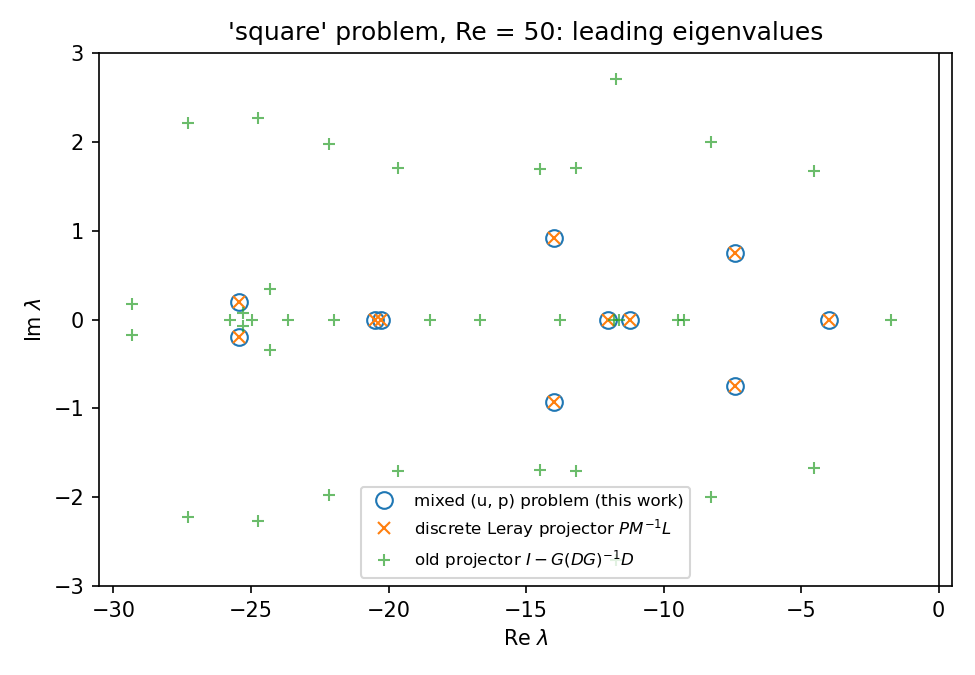
\includegraphics[width=0.76\linewidth,height=90mm,keepaspectratio]{figures/wake_check_projector_equivalence.png}%
}
\expandafter\def\csname reportlayout@figures/membrane_flat_ring_R5_coarse.png\endcsname{%
  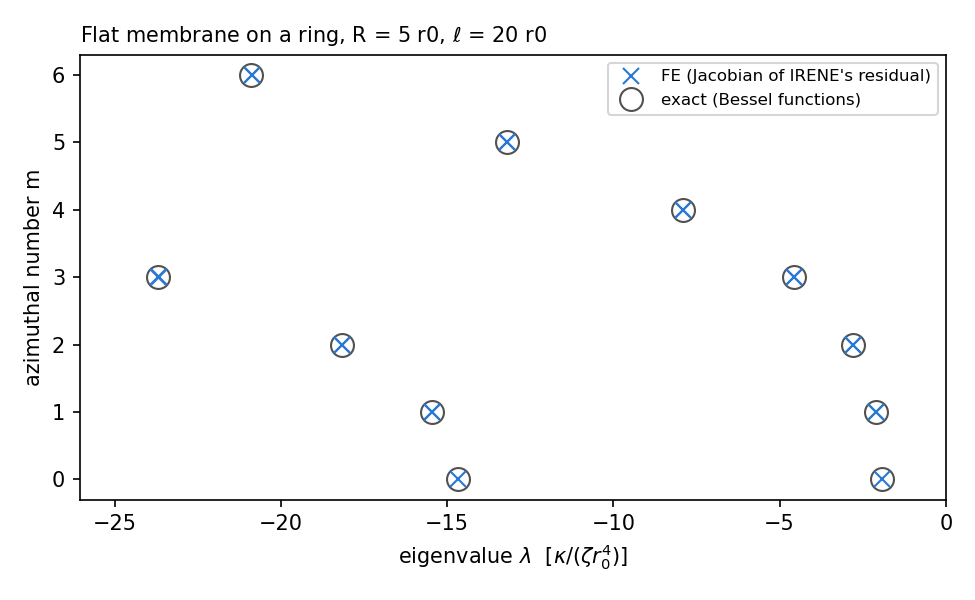
\includegraphics[width=0.70\linewidth,height=82mm,keepaspectratio]{figures/membrane_flat_ring_R5_coarse.png}%
}
\expandafter\def\csname reportlayout@figures/membrane_flat_ring_R5_fine.png\endcsname{%
  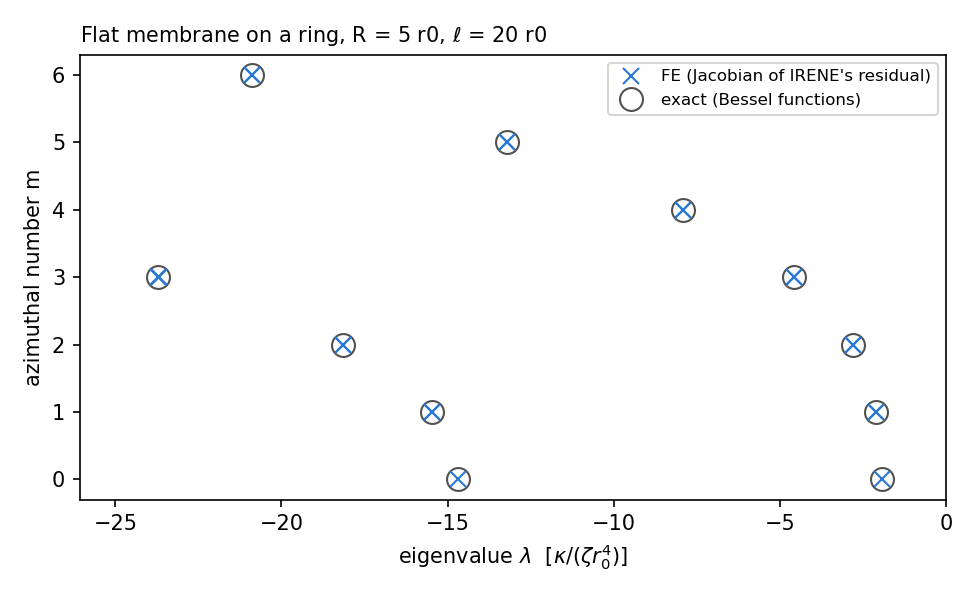
\includegraphics[width=0.70\linewidth,height=82mm,keepaspectratio]{figures/membrane_flat_ring_R5_fine.png}%
}
\expandafter\def\csname reportlayout@figures/wake_spectra.png\endcsname{%
  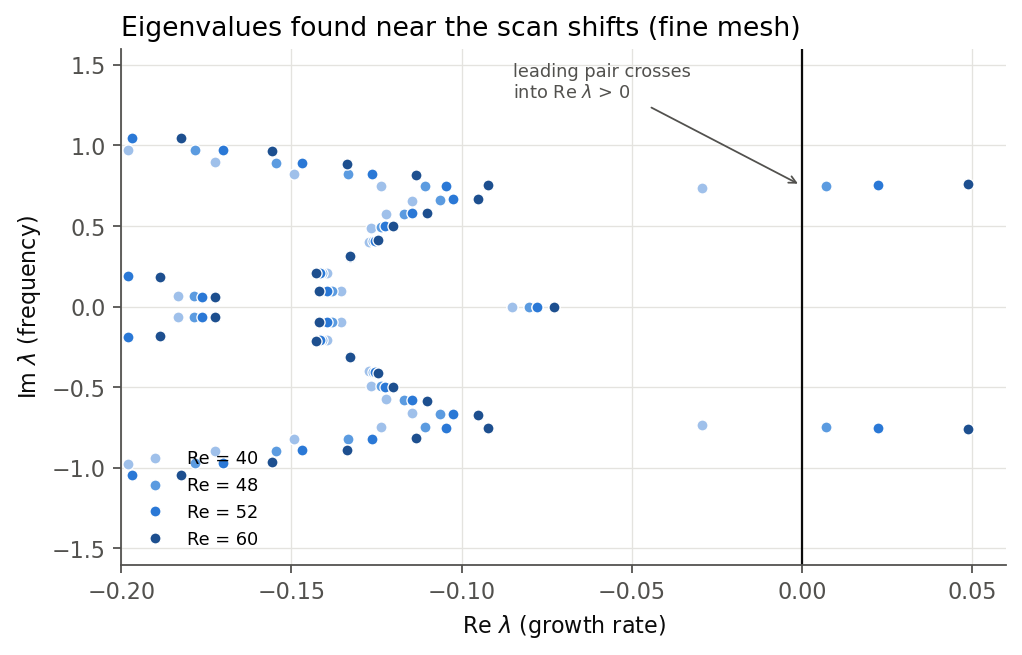
\includegraphics[width=0.78\linewidth,height=100mm,keepaspectratio]{figures/wake_spectra.png}%
}
\expandafter\def\csname reportlayout@figures/wake_eigenvalue_trajectories.png\endcsname{%
  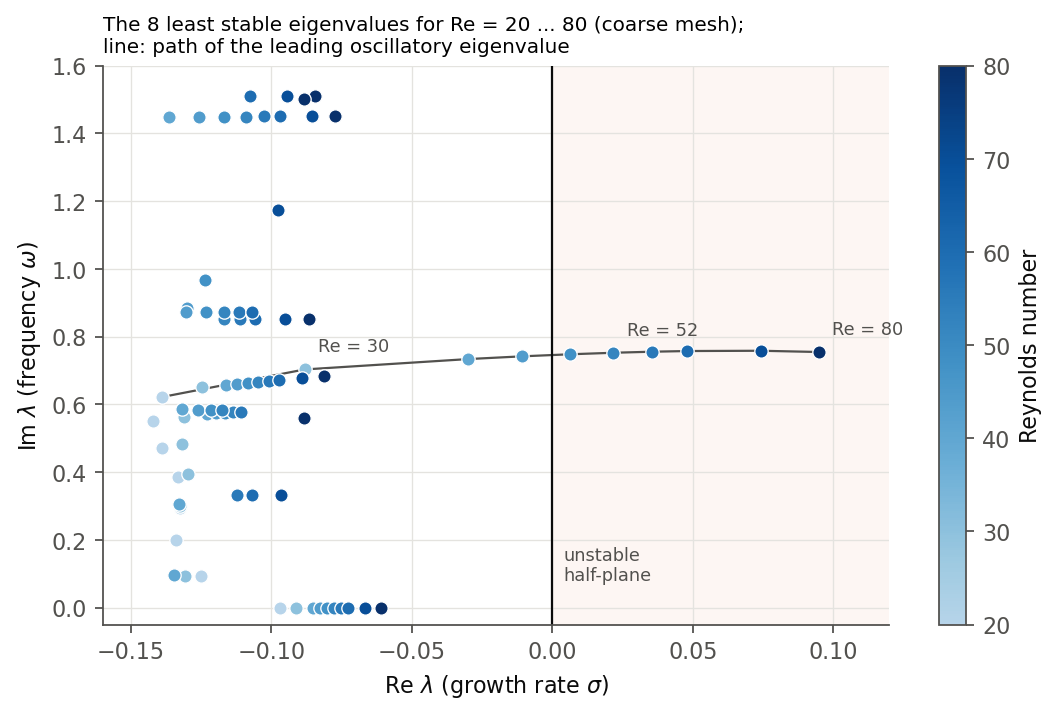
\includegraphics[width=0.78\linewidth,height=100mm,keepaspectratio]{figures/wake_eigenvalue_trajectories.png}%
}
\expandafter\def\csname reportlayout@figures/wake_dns_vorticity.png\endcsname{%
  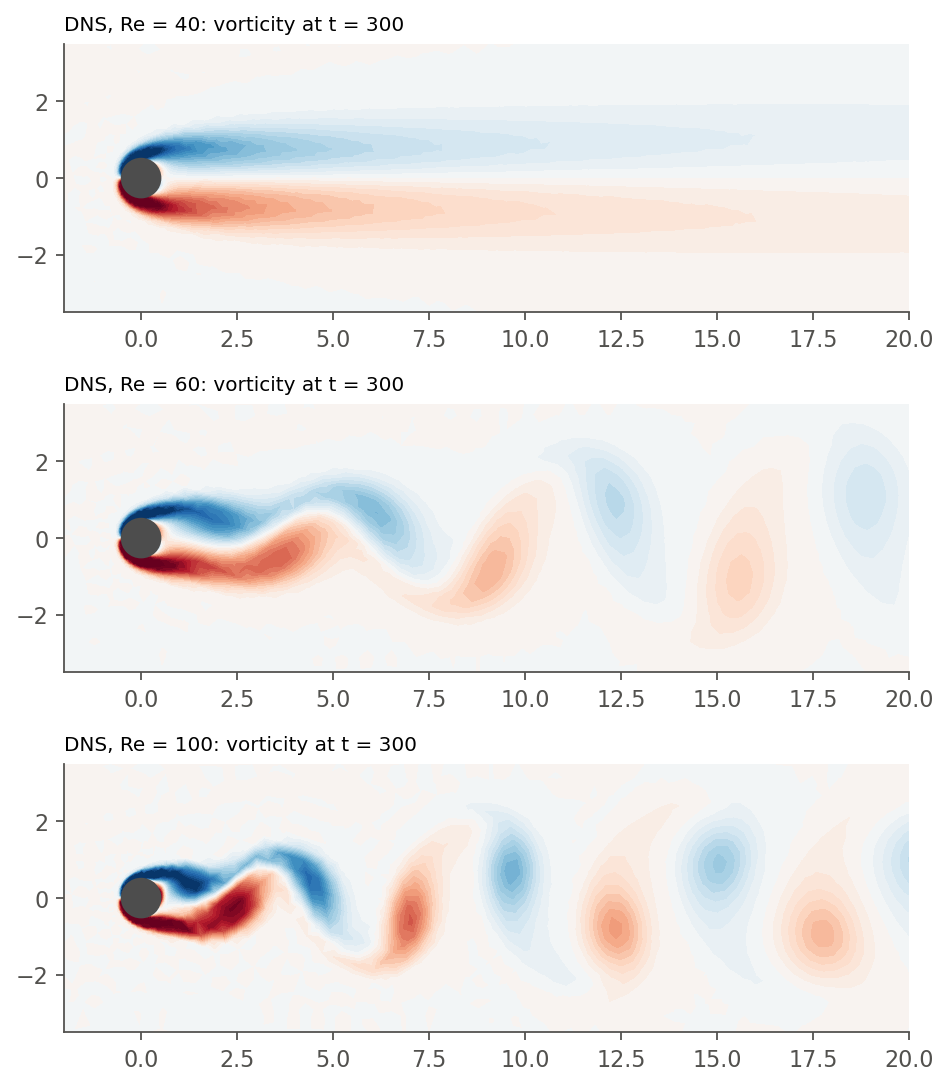
\includegraphics[width=0.64\linewidth,height=112mm,keepaspectratio]{figures/wake_dns_vorticity.png}%
}
\expandafter\def\csname reportlayout@figures/membrane_check_force_methods.png\endcsname{%
  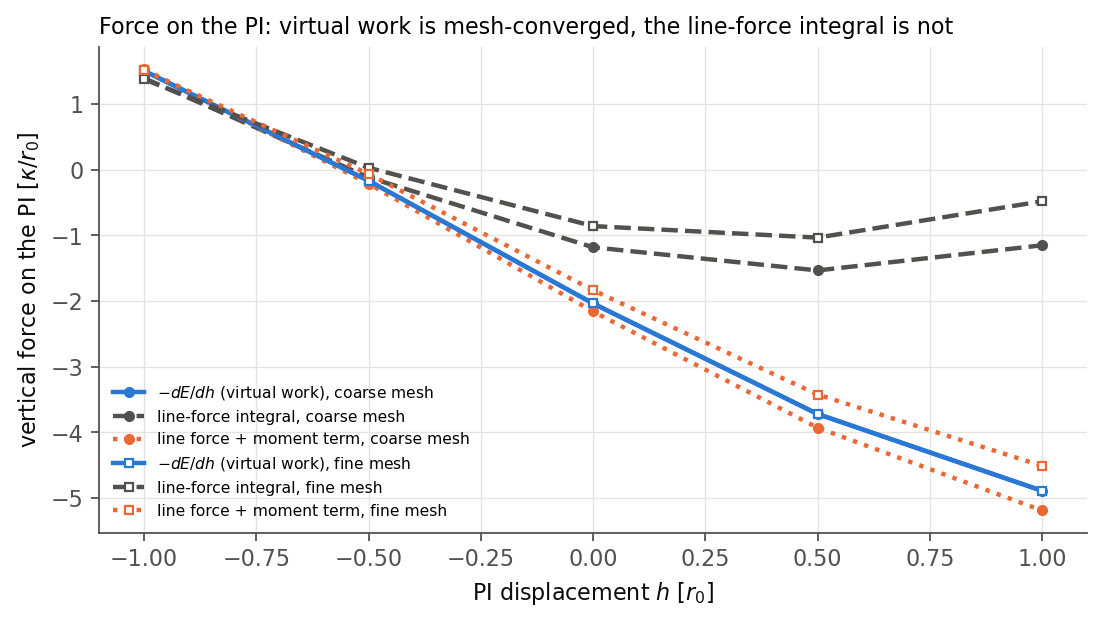
\includegraphics[width=0.82\linewidth,height=92mm,keepaspectratio]{figures/membrane_check_force_methods.png}%
}
\expandafter\def\csname reportlayout@figures/membrane_profiles_ring_R10_tan0.png\endcsname{%
  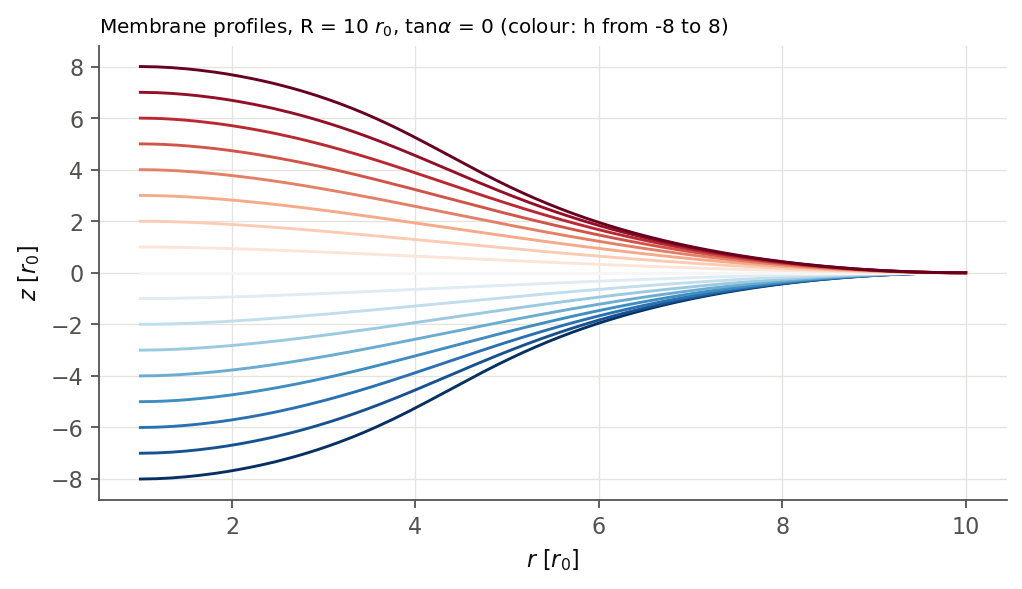
\includegraphics[width=0.76\linewidth,height=85mm,keepaspectratio]{figures/membrane_profiles_ring_R10_tan0.png}%
}
\expandafter\def\csname reportlayout@figures/membrane_profiles_ring_R10_tan0.5.png\endcsname{%
  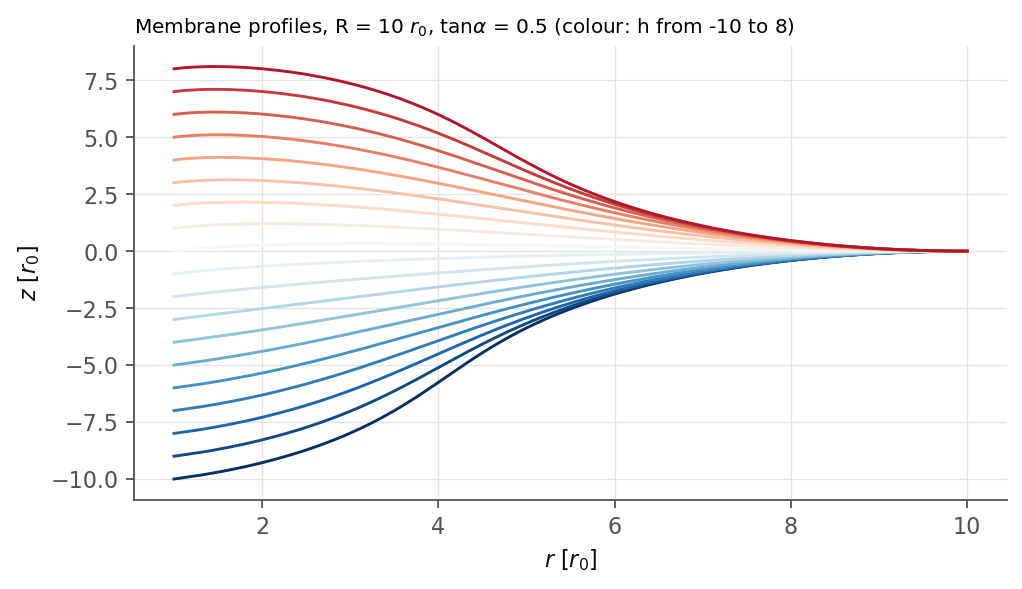
\includegraphics[width=0.76\linewidth,height=85mm,keepaspectratio]{figures/membrane_profiles_ring_R10_tan0.5.png}%
}
\expandafter\def\csname reportlayout@figures/membrane_profiles_ring_R10_tan1.png\endcsname{%
  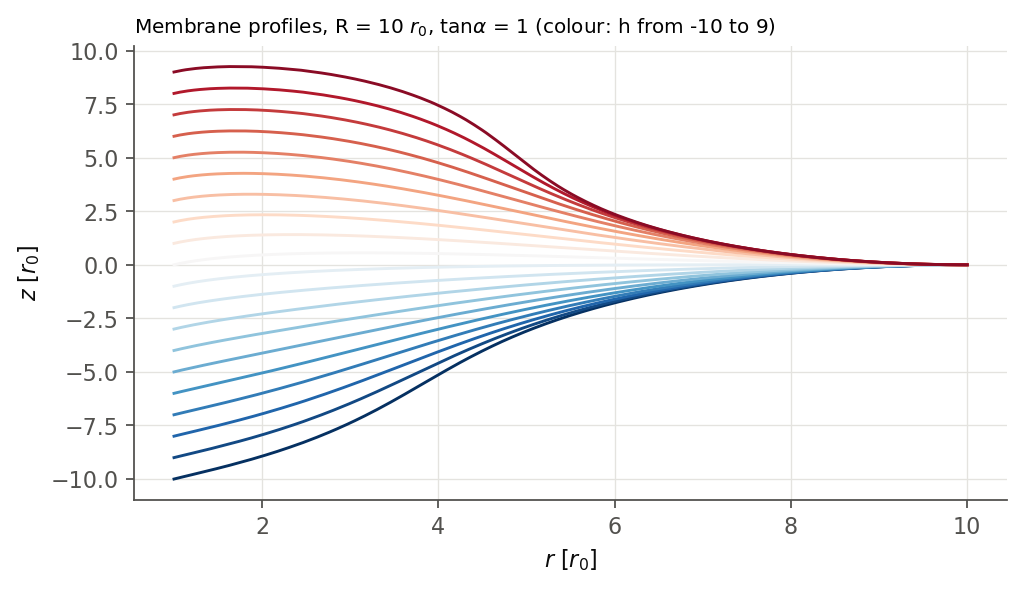
\includegraphics[width=0.76\linewidth,height=85mm,keepaspectratio]{figures/membrane_profiles_ring_R10_tan1.png}%
}
\expandafter\def\csname reportlayout@figures/membrane_profiles_ring_R5_tan0.5.png\endcsname{%
  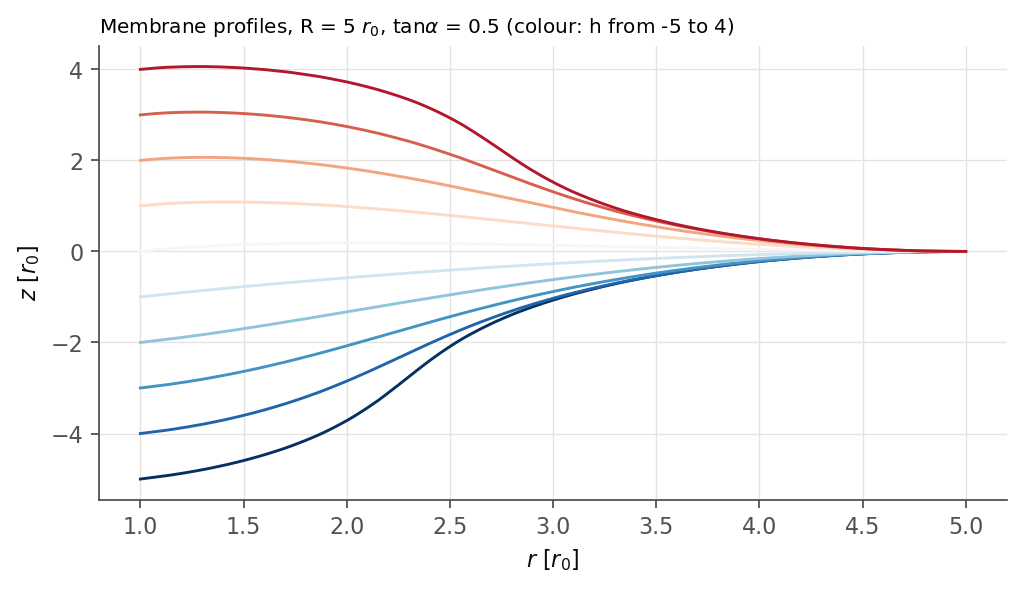
\includegraphics[width=0.76\linewidth,height=85mm,keepaspectratio]{figures/membrane_profiles_ring_R5_tan0.5.png}%
}
\expandafter\def\csname reportlayout@figures/membrane_profiles_ring_R30_tan0.5.png\endcsname{%
  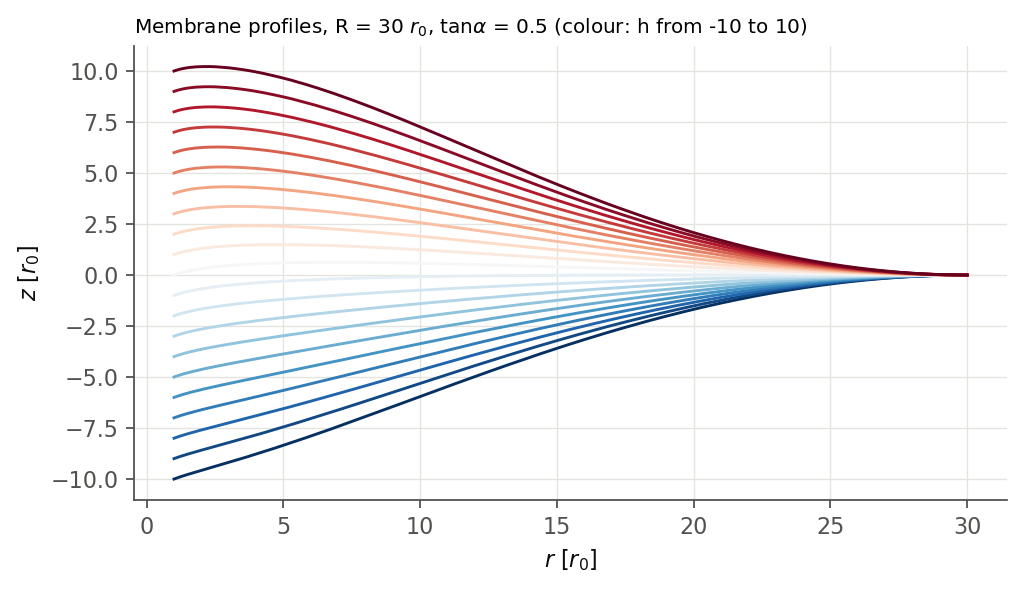
\includegraphics[width=0.76\linewidth,height=85mm,keepaspectratio]{figures/membrane_profiles_ring_R30_tan0.5.png}%
}
\expandafter\def\csname reportlayout@figures/membrane_ring_force_physical_units.png\endcsname{%
  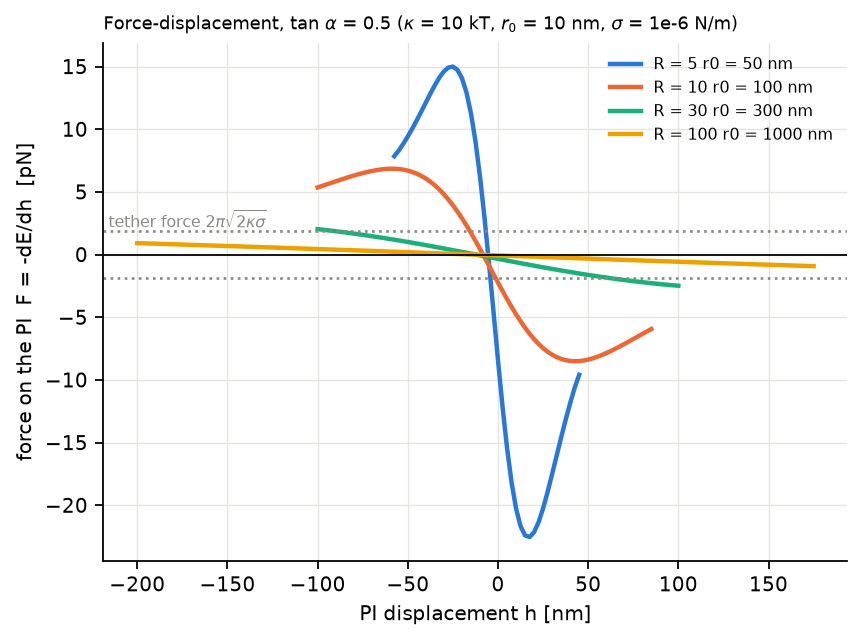
\includegraphics[width=0.72\linewidth,height=105mm,keepaspectratio]{figures/membrane_ring_force_physical_units.png}%
}
\expandafter\def\csname reportlayout@figures/membrane_flow_pre_SLc_vs_tension.png\endcsname{%
  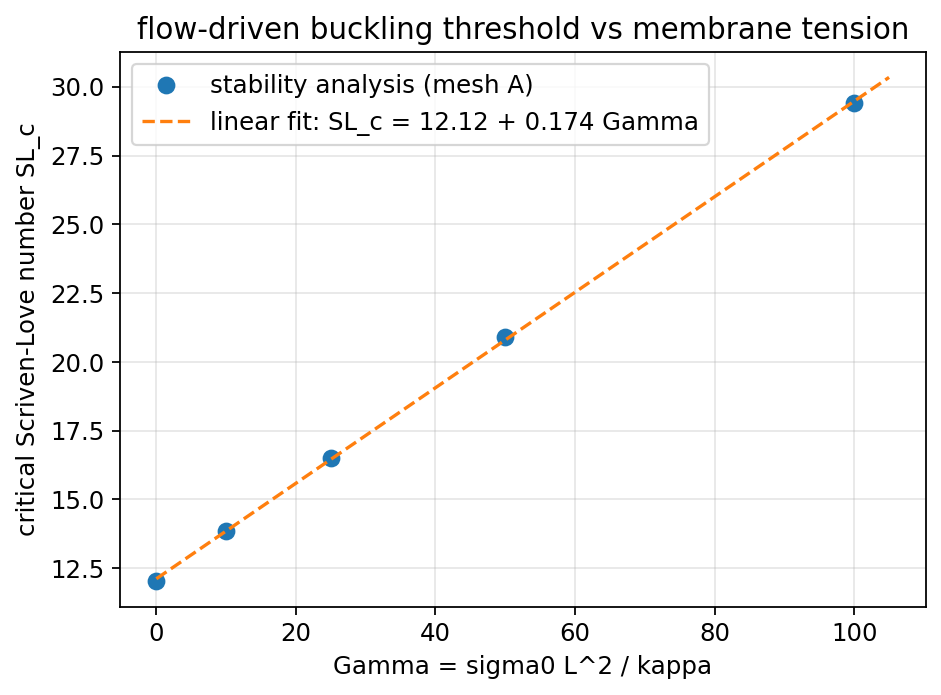
\includegraphics[width=0.70\linewidth,height=100mm,keepaspectratio]{figures/membrane_flow_pre_SLc_vs_tension.png}%
}
\expandafter\def\csname reportlayout@figures/membrane_flow_pre_tension_centreline.png\endcsname{%
  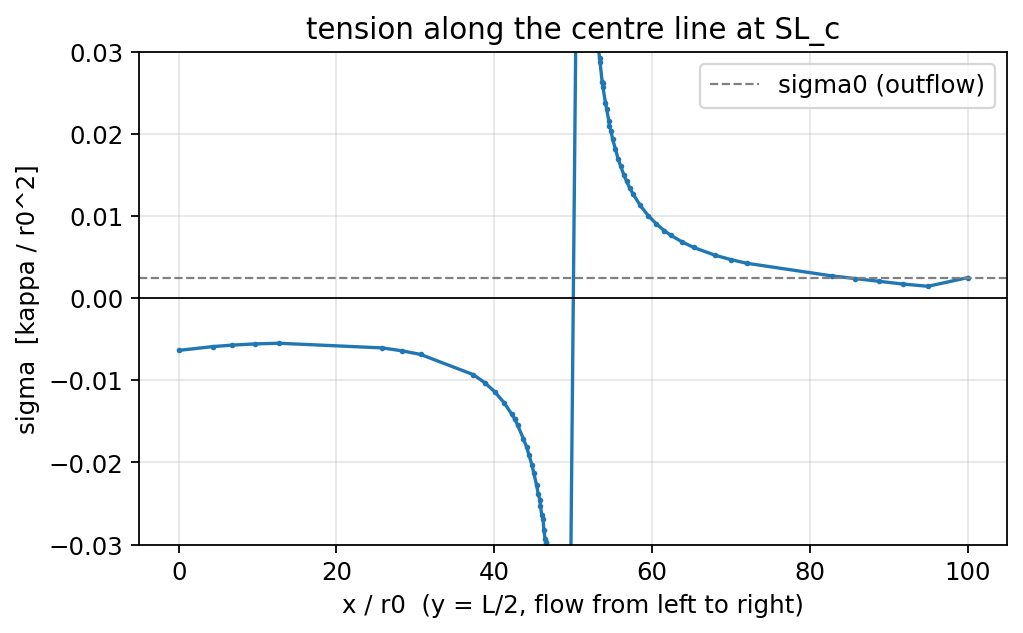
\includegraphics[width=0.66\linewidth,height=90mm,keepaspectratio]{figures/membrane_flow_pre_tension_centreline.png}%
}
\expandafter\def\csname reportlayout@figures/membrane_flow_time_check.png\endcsname{%
  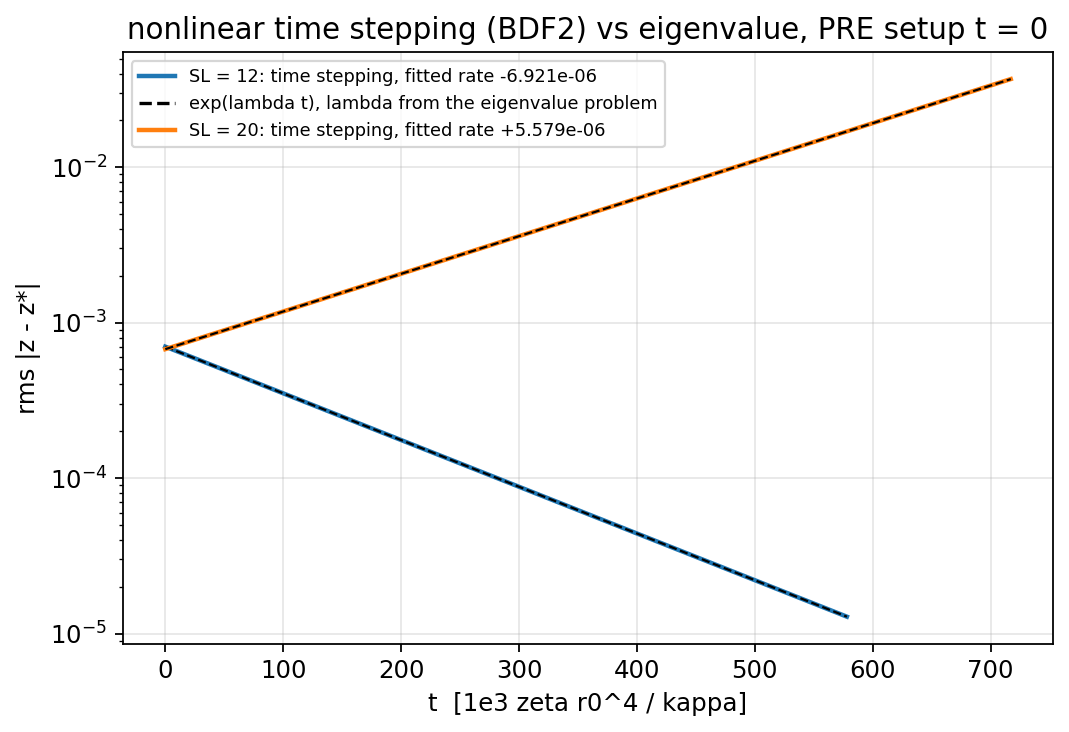
\includegraphics[width=0.76\linewidth,height=100mm,keepaspectratio]{figures/membrane_flow_time_check.png}%
}
\expandafter\def\csname reportlayout@figures/membrane_flow2_threshold_vs_tension.png\endcsname{%
  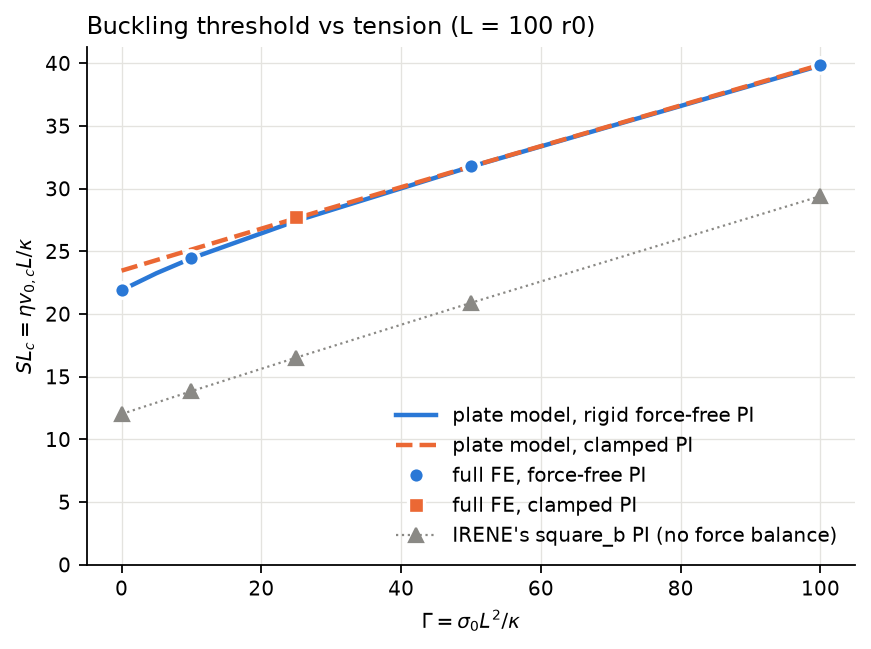
\includegraphics[width=0.70\linewidth,height=100mm,keepaspectratio]{figures/membrane_flow2_threshold_vs_tension.png}%
}
\expandafter\def\csname reportlayout@figures/membrane_flow2_friction.png\endcsname{%
  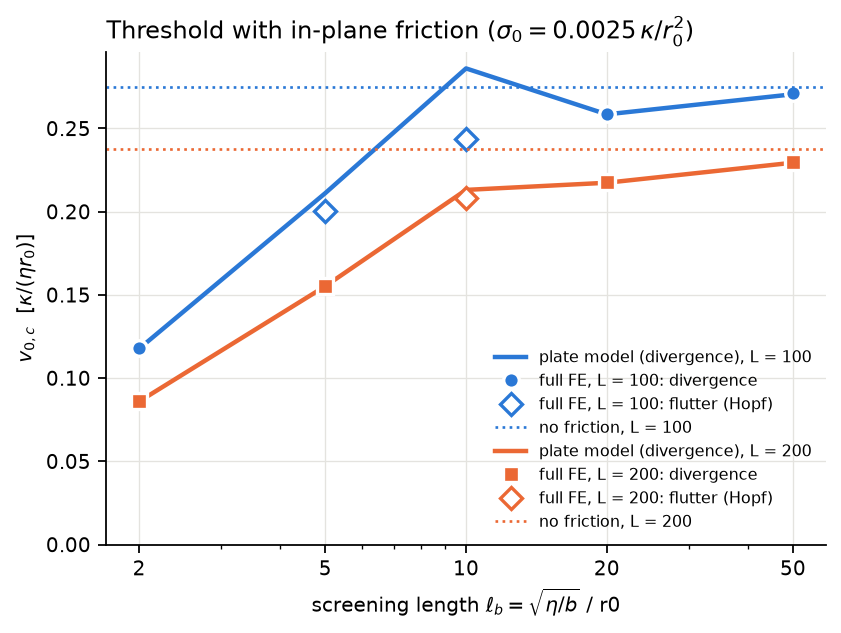
\includegraphics[width=0.72\linewidth,height=100mm,keepaspectratio]{figures/membrane_flow2_friction.png}%
}
\expandafter\def\csname reportlayout@figures/membrane_r6_wake.png\endcsname{%
  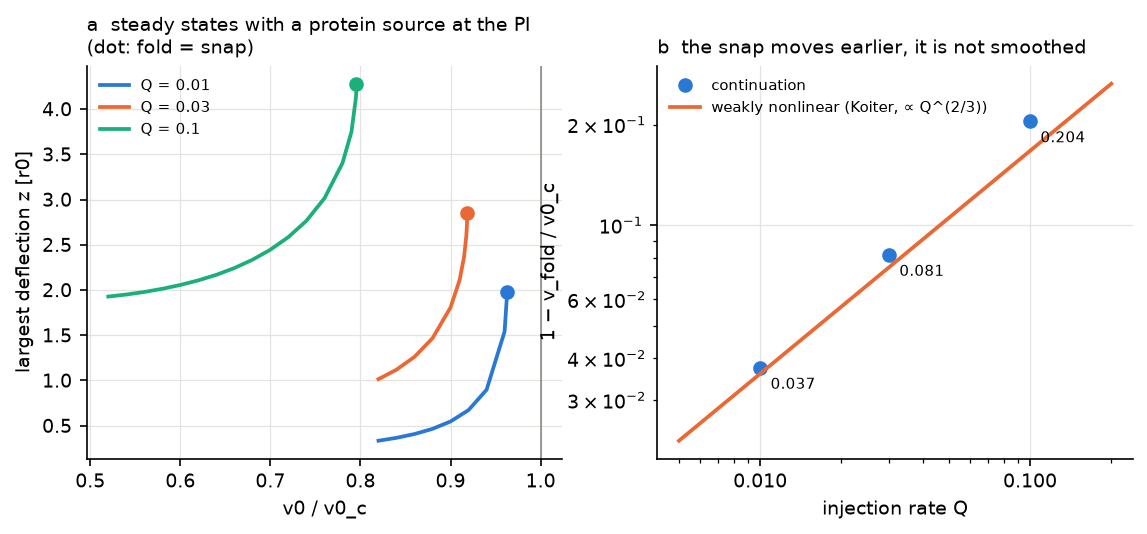
\includegraphics[width=0.86\linewidth,height=75mm,keepaspectratio]{figures/membrane_r6_wake.png}%
}
\expandafter\def\csname reportlayout@figures/membrane_eigenvalues_vs_h.png\endcsname{%
  \reportpanel{figures/membrane_eigenvalues_vs_h.png}{.46\linewidth}{0.000000}{0.000000}{0.795227}{0.000000}{90mm}\hfill
  \reportpanel{figures/membrane_eigenvalues_vs_h.png}{.46\linewidth}{0.204773}{0.000000}{0.595742}{0.000000}{90mm}\par\vspace{2mm}%
  \reportpanel{figures/membrane_eigenvalues_vs_h.png}{.46\linewidth}{0.404258}{0.000000}{0.395970}{0.000000}{90mm}\hfill
  \reportpanel{figures/membrane_eigenvalues_vs_h.png}{.46\linewidth}{0.604030}{0.000000}{0.200343}{0.000000}{90mm}\par\vspace{2mm}%
  \reportpanel{figures/membrane_eigenvalues_vs_h.png}{.46\linewidth}{0.799657}{0.000000}{0.000000}{0.000000}{90mm}\par\vspace{2mm}%
}
\expandafter\def\csname reportlayout@figures/membrane_force_displacement.png\endcsname{%
  \reportpanel{figures/membrane_force_displacement.png}{.46\linewidth}{0.000000}{0.140000}{0.795831}{0.000000}{90mm}\hfill
  \reportpanel{figures/membrane_force_displacement.png}{.46\linewidth}{0.204169}{0.140000}{0.596945}{0.000000}{90mm}\par\vspace{2mm}%
  \reportpanel{figures/membrane_force_displacement.png}{.46\linewidth}{0.403055}{0.140000}{0.395203}{0.000000}{90mm}\hfill
  \reportpanel{figures/membrane_force_displacement.png}{.46\linewidth}{0.604797}{0.140000}{0.199315}{0.000000}{90mm}\par\vspace{2mm}%
  \reportpanel{figures/membrane_force_displacement.png}{.46\linewidth}{0.800685}{0.140000}{0.000000}{0.000000}{90mm}\par\vspace{2mm}%
  \reportpanel{figures/membrane_force_displacement.png}{.88\linewidth}{0.330000}{0.000000}{0.320000}{0.860000}{16mm}%
}
\expandafter\def\csname reportlayout@figures/membrane_ring_stability_diagram.png\endcsname{%
  \reportpanel{figures/membrane_ring_stability_diagram.png}{.47\linewidth}{0.000000}{0.135000}{0.749454}{0.000000}{90mm}\hfill
  \reportpanel{figures/membrane_ring_stability_diagram.png}{.47\linewidth}{0.250546}{0.135000}{0.500218}{0.000000}{90mm}\par\vspace{2mm}%
  \reportpanel{figures/membrane_ring_stability_diagram.png}{.47\linewidth}{0.499782}{0.135000}{0.246614}{0.000000}{90mm}\hfill
  \reportpanel{figures/membrane_ring_stability_diagram.png}{.47\linewidth}{0.753386}{0.135000}{0.000000}{0.000000}{90mm}\par\vspace{2mm}%
  \reportpanel{figures/membrane_ring_stability_diagram.png}{.94\linewidth}{0.245000}{0.000000}{0.245000}{0.865000}{16mm}%
}
\expandafter\def\csname reportlayout@figures/membrane_r3_tube.png\endcsname{%
  \reportpanel{figures/membrane_r3_tube.png}{.47\linewidth}{0.000000}{0.510000}{0.600000}{0.000000}{86mm}\hfill
  \reportpanel{figures/membrane_r3_tube.png}{.47\linewidth}{0.420000}{0.510000}{0.290000}{0.000000}{86mm}\par\vspace{2mm}%
  \reportpanel{figures/membrane_r3_tube.png}{.47\linewidth}{0.000000}{0.000000}{0.600000}{0.490000}{86mm}\hfill
  \reportpanel{figures/membrane_r3_tube.png}{.47\linewidth}{0.740000}{0.510000}{0.000000}{0.000000}{86mm}\par\vspace{2mm}%
}
\expandafter\def\csname reportlayout@figures/membrane_flow_pre_mechanism.png\endcsname{%
  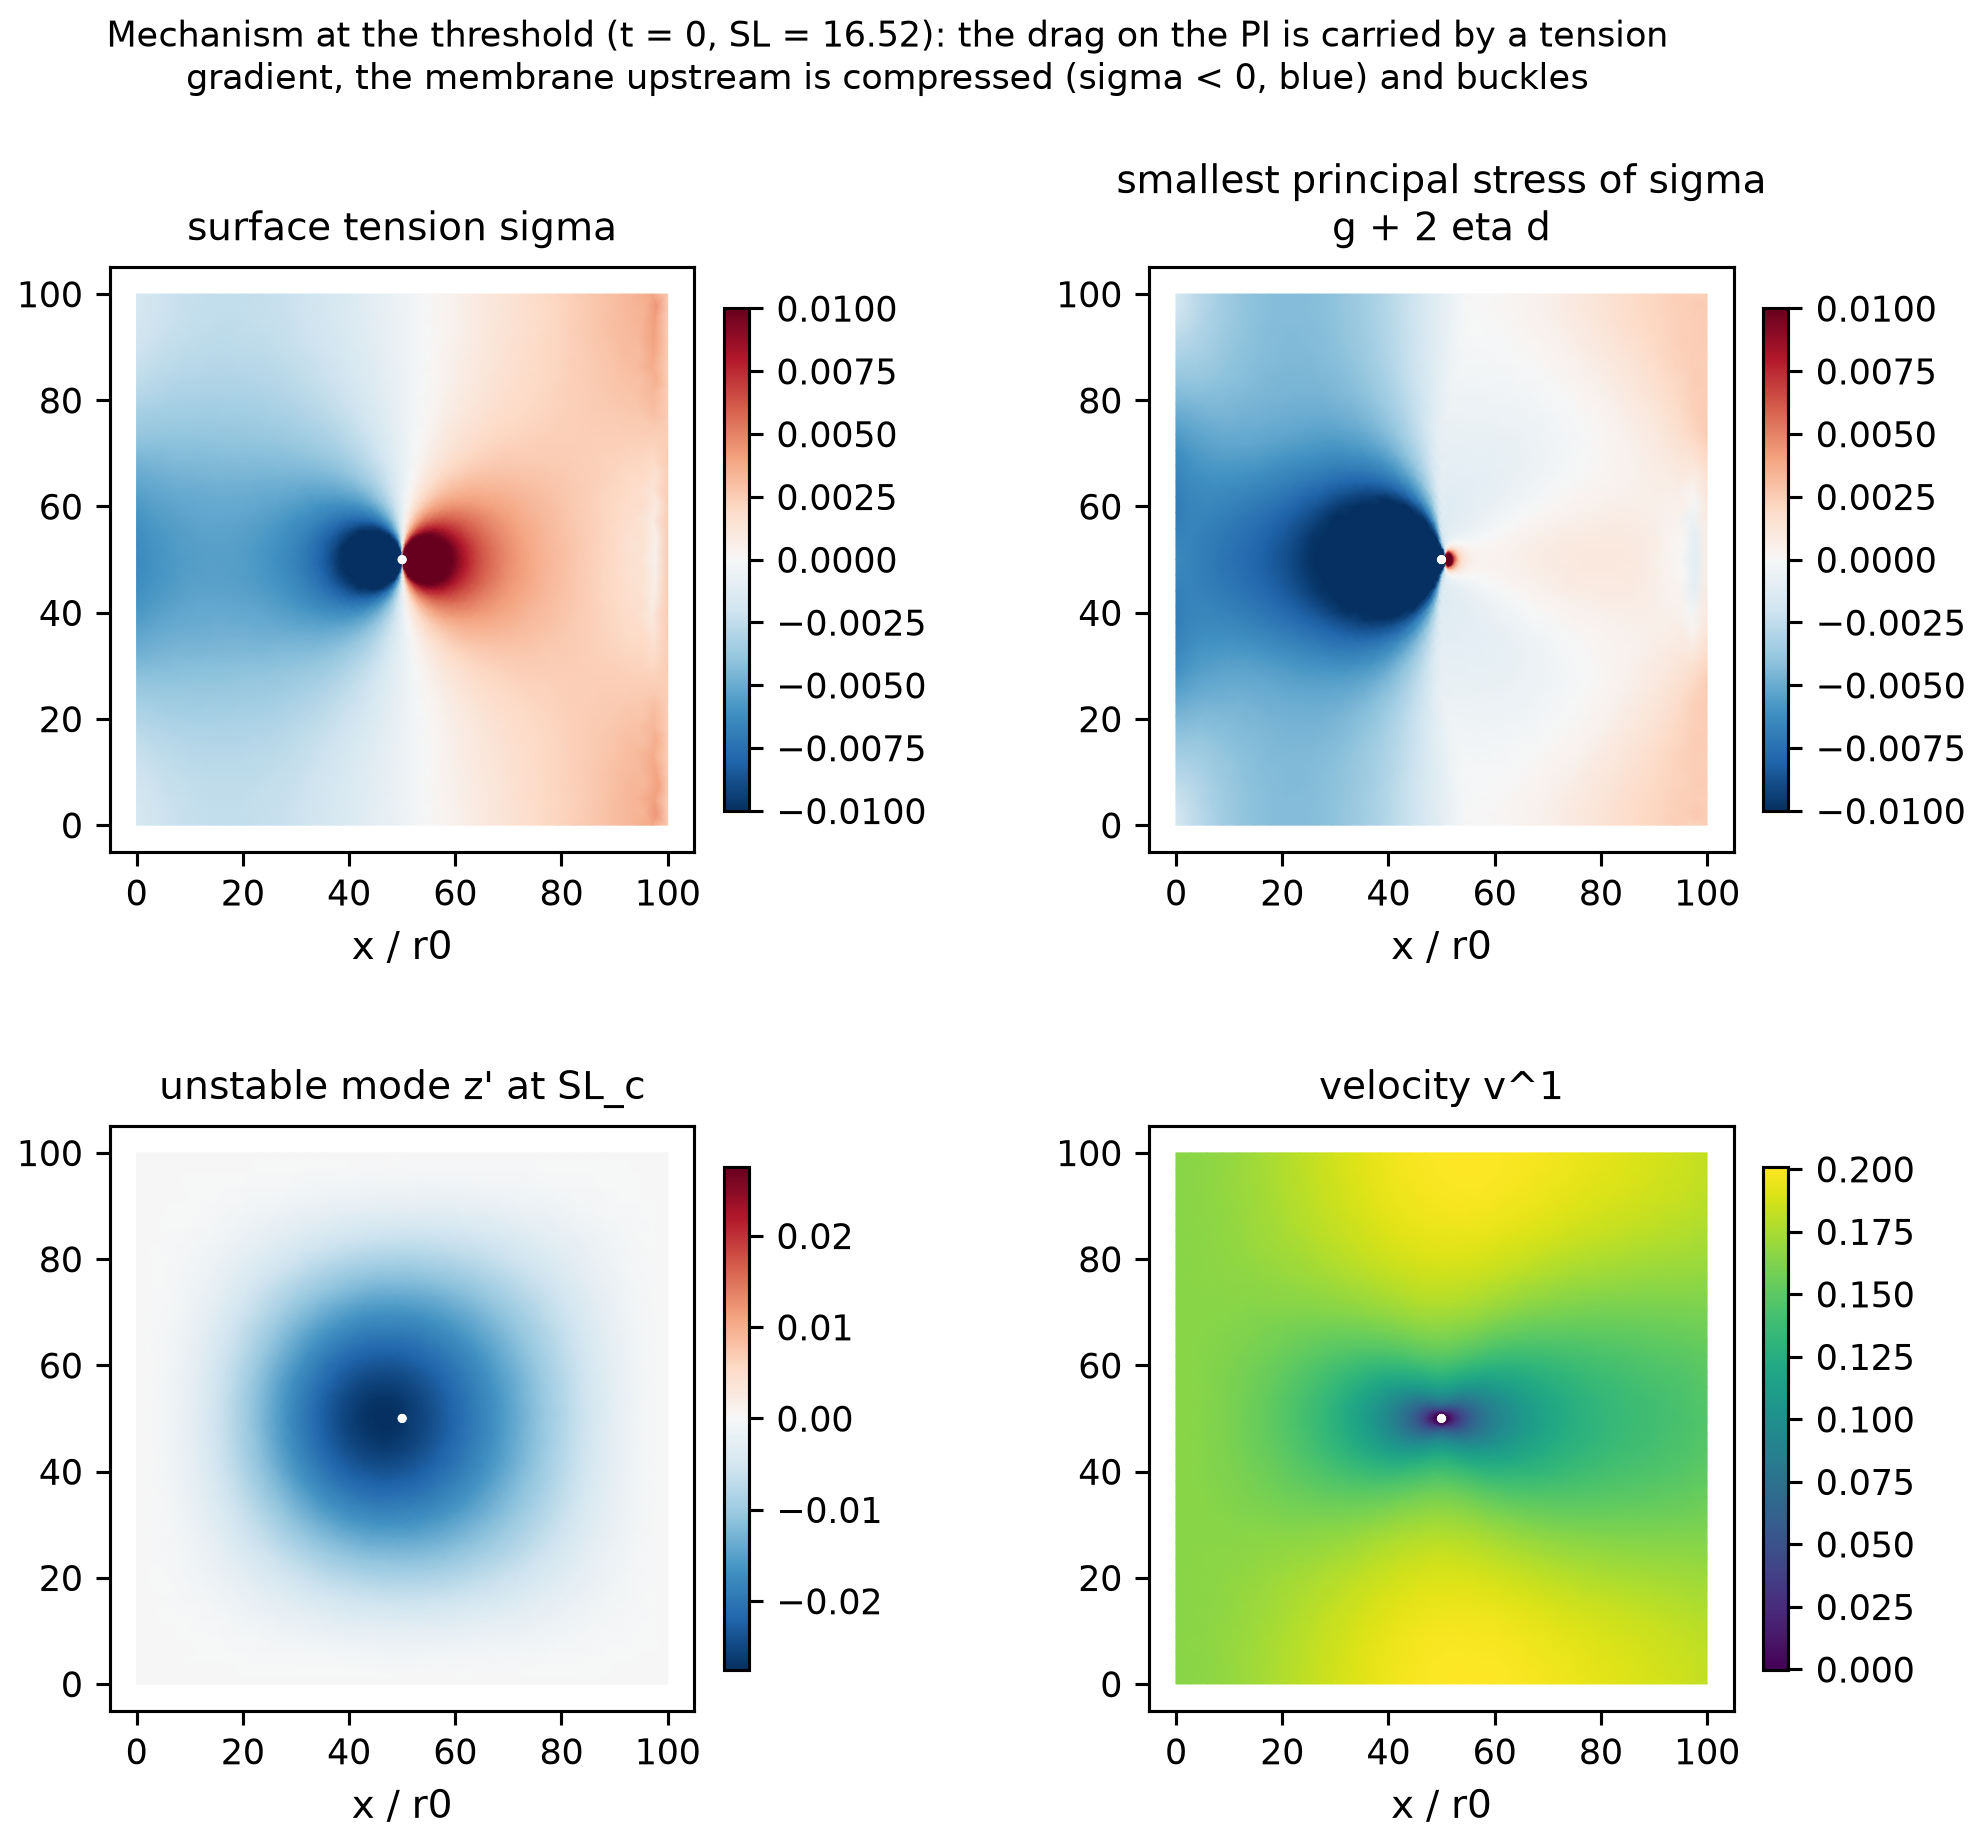
\includegraphics[width=\linewidth,height=140mm,keepaspectratio]{figures/layout/membrane_flow_pre_mechanism.png}%
}
\expandafter\def\csname reportlayout@figures/membrane_flow_pre_imperfect_shapes.png\endcsname{%
  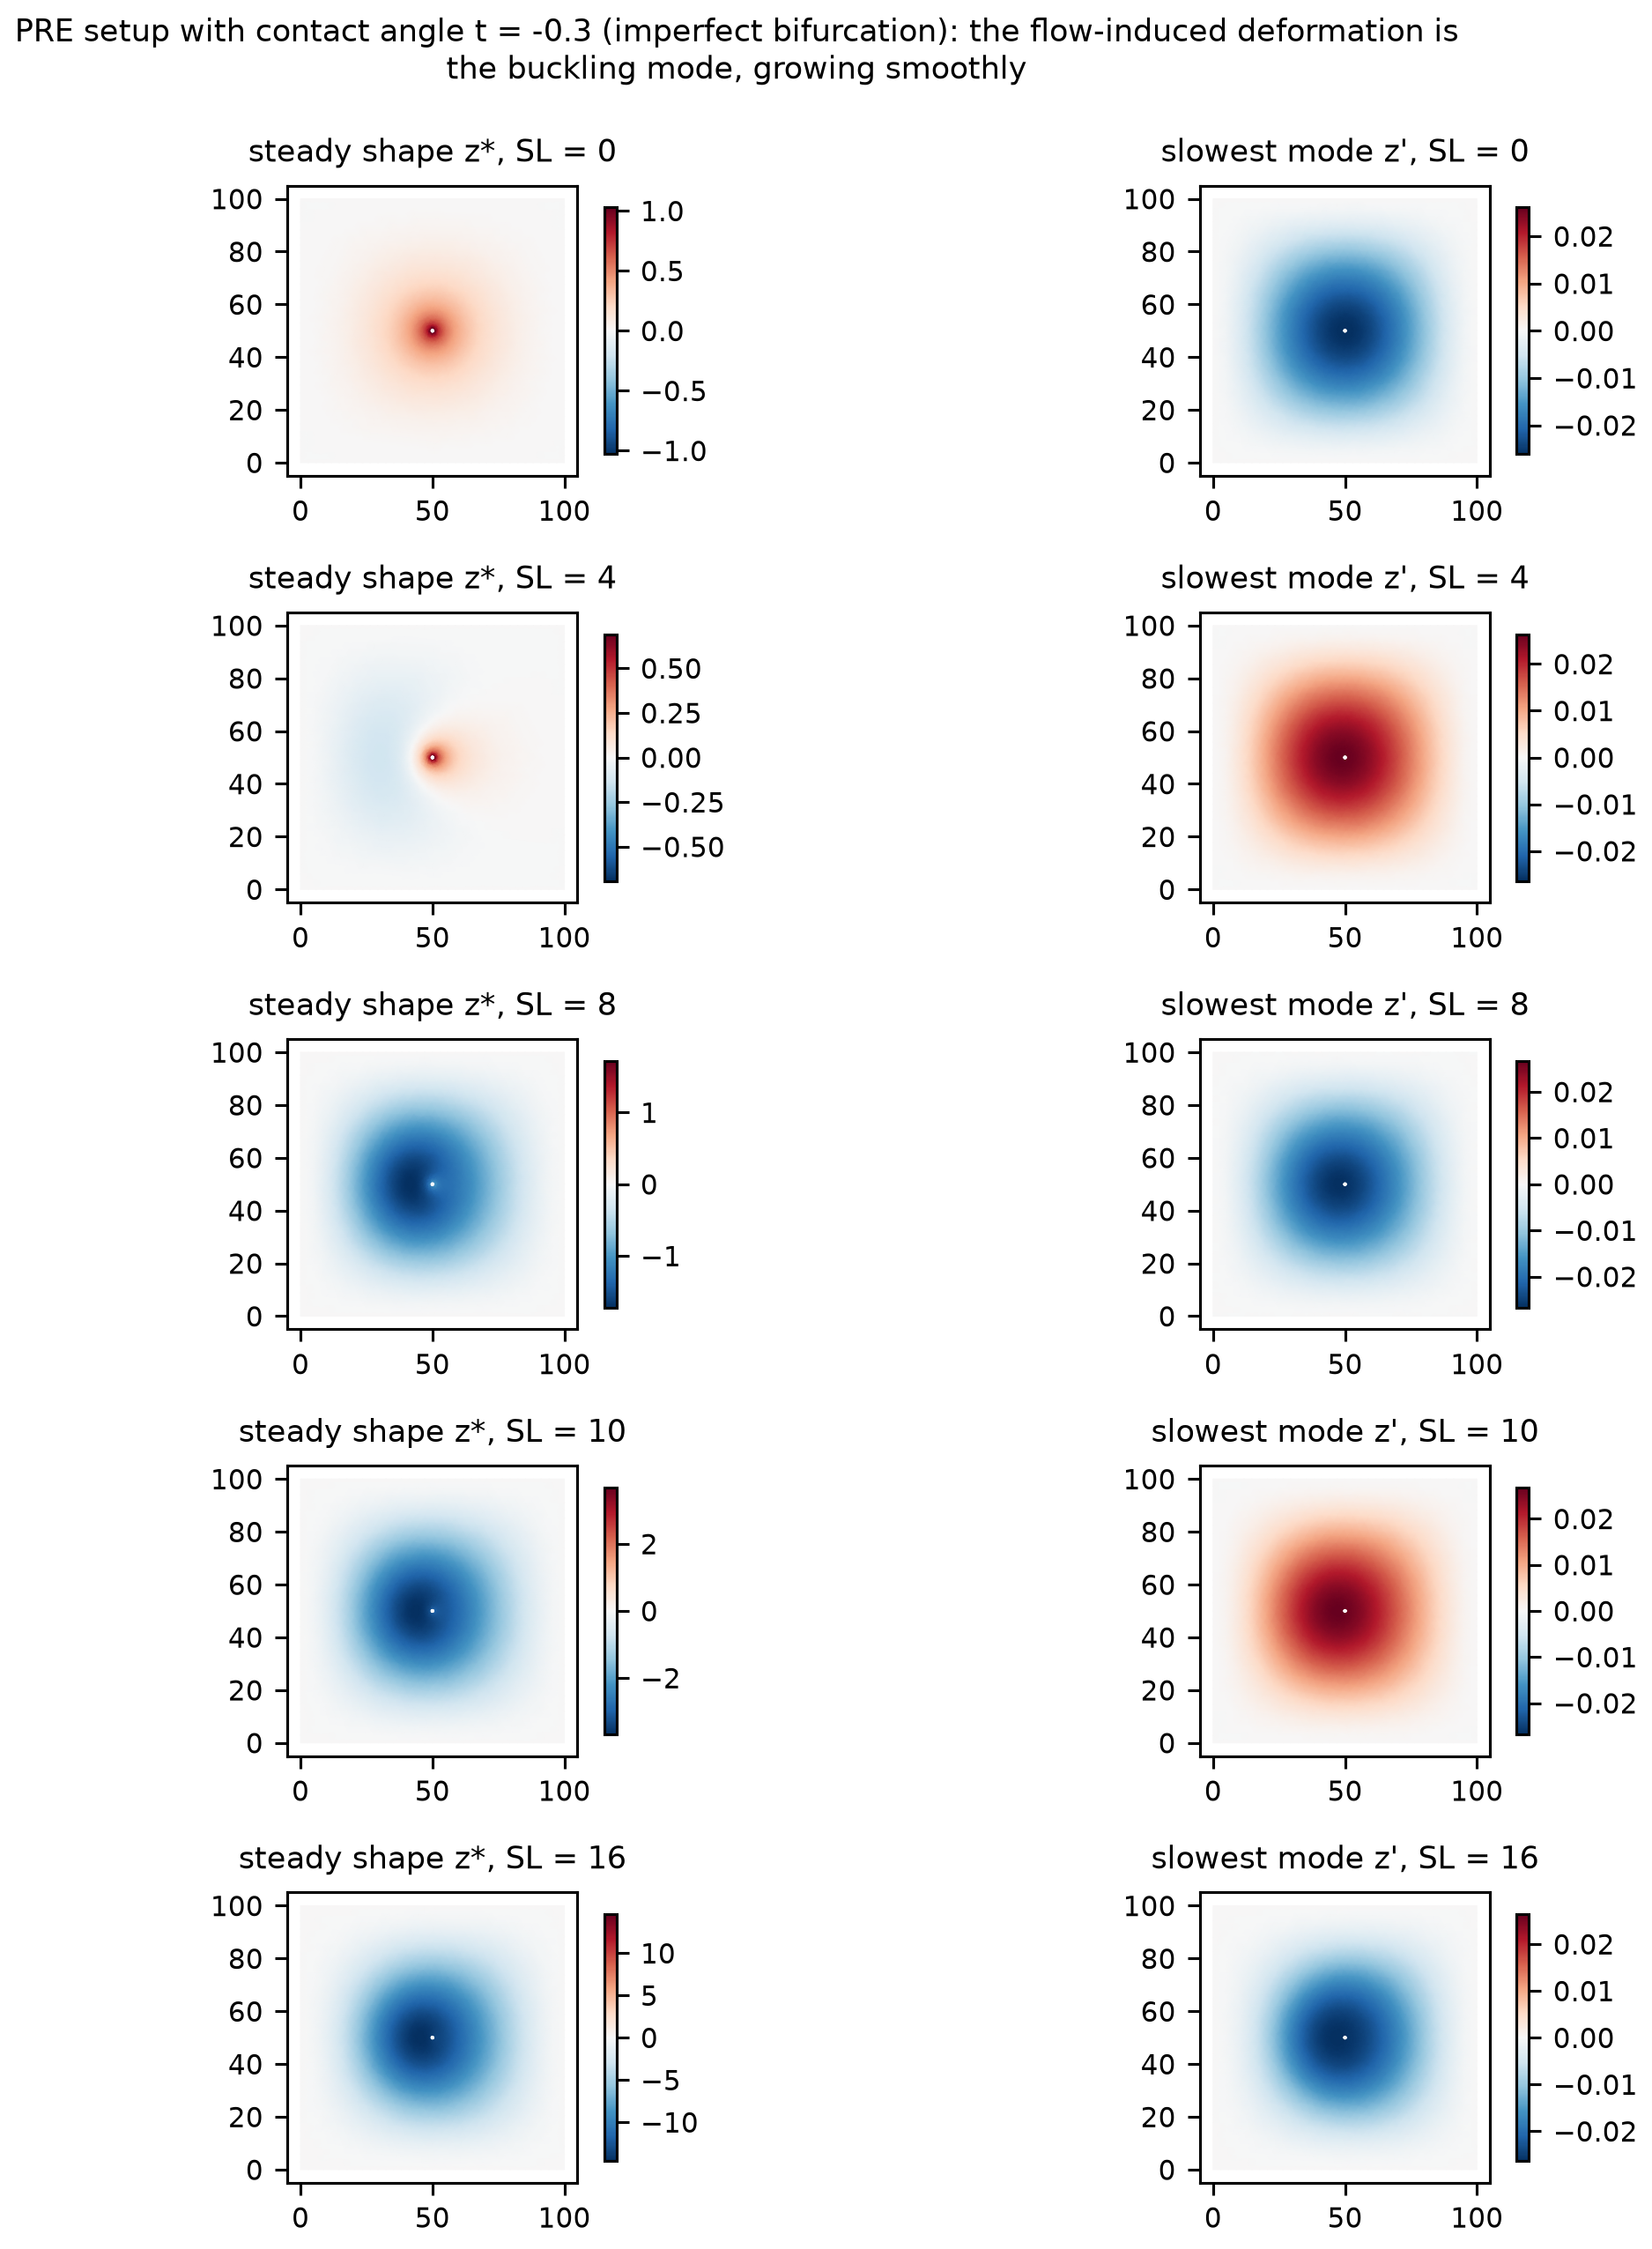
\includegraphics[width=\linewidth,height=220mm,keepaspectratio]{figures/layout/membrane_flow_pre_imperfect_shapes.png}%
}

\begin{document}
\thispagestyle{plain}
\begin{center}
{\LARGE\bfseries\textcolor{ink}{Stability and nonlinear dynamics of flowing\\[3pt] membranes with protein inclusions}}\\[8pt]
{\large From verified eigenvalues to snap-through, flutter, and collective patterns}\\[7pt]
{\small Research report | 4 October 2026}
\end{center}
\begin{abstract}
We develop a stability and nonlinear-dynamics framework for IRENE and use it to determine how a membrane responds to static pulling and tangential flow around anchored proteins. The generalized eigenproblem is obtained by differentiating the mixed finite-element residual and is tested against exact spectra, cylinder-wake instability, independent plate equations, time integration, and mesh refinement. The analysis exposes a missing vertical protein force condition and a nonconvergent boundary-force diagnostic in the inspected implementation. With a physically force-free protein, the reference flow threshold moves from approximately 16 to 27.45 in the dimensionless drive. Obstacle drag lowers upstream tension, producing compressive stress and a subcritical buckling transition. Direct and adjoint projections predict the backward branch and the two-thirds imperfection law without fitting their coefficients. Nonlinear dynamics develops an upstream pit, lifts the protein, and reaches an overhang. Tangential friction instead permits a saturated source of upstream waves. Static ring pulling reveals why a stable height-controlled shape can snap under force control and why confined tether nucleation costs substantially more than the long-tube force. Mobile curvature proteins couple demixing, advection, and buckling; periodic anchored arrays produce density-dependent long-wave instabilities and terrace states in homogenized equations. The analysis connects the governing equations and independently verified stability operator to compression-driven onset, nonlinear snap-through, and collective membrane dynamics. The range of validity of each reduction and the numerical limits of strongly deformed states are specified.
\end{abstract}
\clearpage\tableofcontents\clearpage


\section{Introduction and physical setting}\label{sec:intro}
A stationary membrane shape satisfies force balance but may be unstable to perturbations. We develop a stability operator from IRENE's constrained equations and apply it to static pulling, flow-induced buckling, and their nonlinear extensions. The presentation proceeds from governing equations and verification to physical mechanisms, finite-amplitude evolution, and collective behavior.


\subsection{Equilibrium, linear stability, and nonlinear evolution}
A computed membrane shape answers only the first of three questions. \emph{Existence}: can the forces and geometric constraints balance at this shape? \emph{Stability}: if the shape or flow is disturbed slightly, does it return or depart? \emph{Nonlinear fate}: if it departs, does it settle into another shape, oscillate, or continue to deform? A stationary solver addresses existence; an eigenvalue calculation addresses local stability; continuation and time integration address different parts of the nonlinear fate. The project needed all three because a stationary solver can converge to a shape that would never persist in an experiment.

The simplest analogy is an overdamped displacement $a$ obeying $\zeta\dot a=-ka$. The state $a=0$ solves the stationary equation for either sign of $k$. For $k>0$, a small displacement decays as $\exp(-kt/\zeta)$; for $k<0$, it grows. The membrane has many coupled displacement and flow degrees of freedom, so its restoring coefficient is a matrix rather than one number. Stability analysis identifies the combinations of those degrees of freedom that behave like independent growing or decaying disturbances.

The reference physical system is a membrane patch with a hole occupied by a rigid protein. The protein obstructs membrane flow, and the outer boundary supplies the flow and holds the patch. The protein's radius, the patch size, the bending stiffness, and the imposed tension all matter. Mobile curvature proteins introduced later are a separate field transported over this membrane; they should not be confused with the rigid anchored inclusion. Periodic arrays, introduced last, replace one inclusion and a distant boundary by a repeating arrangement of anchored inclusions.

\subsection{Interpretation of numerical evidence}
Each part below follows a physical question, a mathematical problem, a numerical calculation, and its interpretation. An eigenvalue curve describes small disturbances of a particular base state. A continuation curve describes stationary solutions, including unstable ones. A time trace describes one evolving initial condition. A snapshot shows geometry or a field at one time. These observations address different scales of the dynamics: a nonlinear shape snapshot does not determine an onset threshold, while a linear threshold does not determine the final morphology. The older diagnostic figures remain because they explain how the corrected problem was identified; their boundary conditions are stated where they are discussed.


IRENE provides a finite-element formulation for viscous fluid surfaces \cite{irene}. The large-deformation protein study of Ferraro and Castellana \cite{ferraro} motivates two questions addressed here: which ring-pulling equilibria are stable, and whether sufficiently strong flow destabilizes a membrane around an inclusion. We extend the steady solver with linear spectra, continuation, adjoint projections, and nonlinear dynamics. The central result is a flow-induced snap, with friction-driven flutter as a stable dynamic alternative.


\subsection{Geometry, material parameters, and control variables}


Bending rigidity penalizes curvature, tension penalizes added area, and surface viscosity resists tangential strain rate. Normal friction supplies the dissipation needed to turn a normal restoring force into a shape-relaxation rate. These parameters have different roles: increasing normal friction slows an otherwise unchanged overdamped instability, whereas changing tension alters the restoring stiffness and can move the onset. The dimensionless drive $\SL$ compares flow-induced loading with bending on the stated outer length $L$; $\Gamma$ compares tension with bending on that same length. They are control parameters, not eigenvalues.

Throughout, a prime on a perturbation means a small change from the base state; a prime on a one-variable energy or force means a derivative with respect to that variable. Bold $\bm\omega$ below is a geometric gradient field, while unbold $\omega$ in a complex eigenvalue is a temporal angular frequency. The growth rate is the real part of $\lambda$; the local tension field is $\sigma$. In the cylinder subsection only, $\sigma_{\rm DNS}$ and $\sigma_{\rm eig}$ label fitted and predicted growth rates, and $\mathrm{Re}$ denotes Reynolds number rather than the real-part operator $\Real$.


The membrane has bending rigidity $\kappa$, surface viscosity $\eta$, and imposed reference tension $\sigma_0$. In the Monge representation its surface is $\bm X=(x,y,z)$, with $g_{ij}=\delta_{ij}+z_{,i}z_{,j}$, area element $\dd A=\sqrt g\,\dd x\dd y$, mean curvature $\mathcal H=\tfrac12g^{ij}b_{ij}$, and Gaussian curvature $\mathcal K$. The no-flow energy is
\begin{equation}
E[z]=\int_\Omega(2\kappa\mathcal H^2+\sigma_0)\,\dd A .\label{eq:energy}
\end{equation}
The anchored inclusion is a rigid disc of radius $r_0$: anchoring fixes its lateral position, while its vertical height may be prescribed or force-free. The contact slope is denoted $s=\tan\alpha$; it is not time. For flow through a square of side $L$, the drive and tension parameters are $\SL=\eta v_0L/\kappa$ and $\Gamma=\sigma_0L^2/\kappa$. The reference problem has $L=100r_0$, $\Gamma=25$, no slip on the inclusion, and zero contact slope. Normal friction $\zeta>0$ gives a relaxation time $\tau_n=\zeta r_0^4/\kappa$. In-plane friction $b$, when present, is a separate coupling with screening length $\ell_b=\sqrt{\eta/b}$.


The central mechanism and corrected onset are developed in Sections~\ref{sec:flowhistory}--\ref{sec:geometry}; the nonlinear snap, collapse, fold, and flutter in Sections~\ref{sec:snap}--\ref{sec:flutter}. Sections~\ref{sec:proteins}--\ref{sec:wake} extend the dynamics to mobile curvature proteins, and Sections~\ref{sec:lattice}--\ref{sec:terraces2d} treat collective anchored arrays. The preceding methods and static results provide the force conventions and validation on which those interpretations depend.


The distinction between existence and stability can be stated compactly as
\begin{equation}
\mathcal R(\Psi_*;p)=0,\qquad
\gamma_{\max}(p)=\max_{\lambda\in\mathrm{spec}_{\rm phys}}\Real\lambda,
\qquad \gamma_{\max}(p_c)=0.
\label{eq:onset-definition}
\end{equation}
$p$ is the chosen control parameter, and the maximum is over admissible finite physical modes, excluding an identified symmetry mode. Below a simple stable onset $\gamma_{\max}<0$; locating $p_c$ therefore requires solving the base problem and its spectrum at successive controls. No value of $p_c$ follows from $\mathcal R=0$ alone.

\subsection{Scope and organization}
The analysis begins with the generalized stability problem and its verification. Static ring pulling establishes the distinction between height and force control. The force-balanced flow problem then connects obstacle drag, upstream compression, and buckling. Stationary continuation and mode projection determine the local snap-through structure, while time integration and parametric geometry follow the departure into strongly deformed states. Tangential friction, mobile curvature-coupled composition, and periodic inclusion arrays extend the same framework to oscillatory and collective dynamics.

Boundary conditions define the physical problem: a deformable free rim, a rigid force-free inclusion, and a prescribed protein height permit different disturbances. Linear onset, local nonlinear criticality, and the eventual large-amplitude state are therefore assessed separately. In particular, a destabilizing cubic coefficient characterizes the nearby branch but does not determine a terminal shape. Similarly, terrace stability in a homogenized equation is established within that reduction and requires separate verification in a fully coupled microscopic model.

\section{Governing geometry and a stability operator from IRENE}\label{sec:operator}
The method treats stability as a property of the actual constrained residual. This avoids substituting a guessed shape equation for a mixed viscous-surface discretization and makes boundary and force inconsistencies visible in the spectrum.


\subsection{Perturbations and modal growth rates}
Let $\Psi_*$ denote the complete stationary state: not just the height, but also the velocities, tension, curvature variables, and any additional coupled fields. It satisfies the discrete force and constraint equations $\mathcal R(\Psi_*)=0$. We ask what happens to a small disturbance $\delta\Psi$, while keeping the imposed boundary drive and the physical control conditions unchanged. Linearization keeps terms proportional to $\delta\Psi$ and discards terms quadratic or higher in its size. It is a local approximation about this one stationary state.

A normal mode separates spatial structure from time dependence:
\begin{equation}
\delta\Psi(t)=\varepsilon\,\Real\{x\exp(\lambda t)\},\qquad
\lambda=\gamma+i\omega.
\label{eq:reading-mode}
\end{equation}
The vector $x$ specifies the disturbance of every field at every mesh degree of freedom. Its height component shows where the membrane bends; its velocity and tension components show the accompanying response. The real part $\gamma$ is the growth rate, and $\omega$ is the angular frequency. A negative growth rate means decay, a positive one means instability, and a zero one means neutral stability at linear order. If $\omega\ne0$, the real disturbance oscillates as it grows or decays, with period $2\pi/|\omega|$. With a complex eigenvector, the real and imaginary spatial patterns are a quarter-period apart; plotting only one part does not show the whole cycle.

The \emph{leading} physical mode is the one with the largest growth rate among the admissible finite eigenvalues. A static buckling onset occurs when a real eigenvalue passes through zero. A Hopf onset occurs when a complex-conjugate pair crosses the imaginary axis at a nonzero frequency. A rigid translation allowed by the boundary conditions can instead produce a neutral mode for every drive; that mode must be recognized before interpreting zero as a buckling threshold. Eigenvector amplitude is arbitrary in a linear calculation, so a plotted mode is a shape of a disturbance, not a prediction of its eventual depth.

\subsection{Finite-element representation and weak residual}
\label{sec:fem-detail}
The finite-element method (FEM) turns a field problem into equations for a finite collection of coefficients. It does not replace the membrane by independent point particles. Neighboring coefficients are coupled by integrals of the governing equations over a triangulation $\mathcal T_h$ of the reference domain $\Omega$. Here $h$ denotes a characteristic element size, not the protein height. On a curved height graph, the triangles are in reference $(x,y)$ coordinates; the metric and $\sqrt g$ in each integral account for physical surface lengths and areas.

\paragraph{Fields, basis functions, and degrees of freedom.}
For a scalar field $f$, continuous piecewise-polynomial spaces are
\begin{equation}
V_h^{(p)}=\{f_h\in C^0(\overline\Omega):f_h|_K\in\mathbb P_p(K)
\text{ for every }K\in\mathcal T_h\},\qquad
f_h(\bm x)=\sum_{j=1}^{N_f}F_jN_j^{(f)}(\bm x).
\label{eq:fem-space}
\end{equation}
$\mathbb P_p(K)$ contains polynomials of total degree at most $p$ on triangle $K$, $N_j^{(f)}$ is a basis function, and $F_j$ is its unknown coefficient. For standard nodal $P_1$ elements, these coefficients are the values at triangle vertices. For $P_2$, they also include values at edge midpoints. A vector field has a copy of the scalar space for each component. Shared vertex/edge coefficients enforce continuity between neighboring triangles; derivatives need not be continuous across their edges.

For example, let $\ell_1,\ell_2,\ell_3$ be barycentric coordinates on a triangle, satisfying $\ell_1+\ell_2+\ell_3=1$. Its three $P_1$ functions are $\ell_i$, and its six $P_2$ functions are
\begin{equation}
N_i=\ell_i(2\ell_i-1)\quad(i=1,2,3),\qquad
N_{ij}=4\ell_i\ell_j\quad(ij=12,23,31).
\end{equation}
Mapping a reference triangle to each physical reference-domain triangle transforms their derivatives. Thus mesh refinement increases the number and spatial resolution of permissible disturbances; it does not merely improve an eigenvalue search on an unchanged matrix.

The full state belongs to a product of spaces, one for each field. For the flow calculation described here,
\begin{equation}
\mathcal V_h=[V_h^{(2)}]^2\times V_h^{(1)}\times V_h^{(1)}
\times V_h^{(1)}\times[V_h^{(1)}]^2\times V_h^{(1)},
\qquad \Psi_h=(\bm v_h,w_h,\sigma_h,z_h,\bm\omega_h,\mu_h).
\end{equation}
The order of the factors matches the displayed unknowns. Their concatenated coefficient vector is $\bm U$; its length is the sum of all field degrees of freedom. A mixed vector includes velocity, constraint, and geometry components, so a height-only disturbance is generally not an admissible eigenvector until the other fields have adjusted.

\paragraph{Weak equations and boundary work.}
A weak equation is required to hold against every admissible test function. Integration by parts transfers derivatives from an unknown to a test function and exposes boundary fluxes. For example,
\begin{equation}
\int_\Omega q\,\Delta z\,\dd^2x
=-\int_\Omega\nabla q\cdot\nabla z\,\dd^2x
+\oint_{\partial\Omega}q\,\partial_nz\,\dd\ell.
\label{eq:fem-parts}
\end{equation}
The boundary integral must be retained, eliminated by the stated boundary data, or replaced by the consistent natural boundary condition. It cannot be discarded because it is inconvenient. Tests vanish on an essential boundary where the corresponding unknown is prescribed; a free rigid protein instead admits a shared rim displacement, and its test equation must include the resulting total reaction.

The fourth-order bending equation illustrates why a mixed representation is useful. In the flat limit, $2\mathcal H=\Delta z$. Introduce a Laplacian field $m_\Delta$ and consider the conservative plate with zero prescribed slope and admissible homogeneous tests $q,\xi$. Its two weak equations are
\begin{align}
&\int_\Omega m_\Delta q\,\dd^2x+
\int_\Omega\nabla z\cdot\nabla q\,\dd^2x=0,\\
&\zeta\int_\Omega z_t\xi\,\dd^2x
-\kappa\int_\Omega\nabla m_\Delta\cdot\nabla\xi\,\dd^2x
+\int_\Omega\nabla\xi\cdot\mathsf T\nabla z\,\dd^2x=0.
\label{eq:fem-mixed-plate}
\end{align}
The first equation imposes $m_\Delta=\Delta z$ weakly. The second is $\zeta z_t+\kappa\Delta m_\Delta-\nabla\cdot(\mathsf T\nabla z)=0$ after integration by parts and the appropriate boundary treatment. Each integral requires first derivatives only, so continuous elements suffice. This is an explanatory flat-plate example: the independent plate solver uses $P_2\times P_2$, whereas IRENE uses separate $\bm\omega$ and $\mu$ fields with its nonlinear geometric and boundary forms. It would be incorrect to substitute this example for those full forms or to omit follower forcing when the base stress is not divergence-free.

In the full formulation, the independent gradient and curvature are constrained, rather than additional freely chosen material fields. At the continuum level their identities are
\begin{equation}
\bm\omega=\nabla z,\qquad
2\mu=\nabla\cdot\left(\frac{\bm\omega}{\sqrt{1+|\bm\omega|^2}}\right),
\qquad \nabla_i v^i-2\mu w=0.
\end{equation}
The second identity uses the upward normal of the height graph. The corresponding mixed weak rows and boundary terms impose these identities in the discrete space. The tension $\sigma$ is a Lagrange multiplier for the last constraint. Its role is analogous to pressure in incompressible flow, although the membrane stress uses the tensile-positive convention.

\paragraph{From weak forms to an assembled residual.}
Denote the weak residual by $\mathcal R(\Psi_h;\nu_h)$; it is nonlinear in the state but linear in the test collection $\nu_h$. Choosing each basis test $\nu_i$ gives
\begin{equation}
R_i(\bm U)=\mathcal R(\Psi_h(\bm U);\nu_i)
=\sum_{K\in\mathcal T_h}R_i^{K}(\bm U)
+\sum_{e\subset\partial\Omega}R_i^{e}(\bm U).
\label{eq:fem-residual}
\end{equation}
Element contributions are accumulated into the global rows sharing their degrees of freedom. Volume quadrature approximates integrals on triangles and boundary quadrature approximates those on edges. Geometry, viscosity, curvature, friction, and penalty terms all contribute to these local integrals. The flow interface sets quadrature degree four for its nonlinear forms; mesh convergence and, where needed, quadrature sensitivity are separate from convergence of the algebraic solver.

A stationary calculation solves $\bm R(\bm U_*)=0$. Newton iteration uses
\begin{equation}
\mathsf J(\bm U^{(k)})\Delta\bm U=-\bm R(\bm U^{(k)}),
\qquad \mathsf J_{ij}=\frac{\partial R_i}{\partial U_j},
\qquad \bm U^{(k+1)}=\bm U^{(k)}+\Delta\bm U.
\end{equation}
Boundary data and rigid constraints are included in this solve. A small Newton residual means force and constraint balance in this discrete space; it gives no sign information about physical disturbance growth.

\paragraph{Linearization of the assembled dynamic problem.}
The time form is another weak expression, $\mathcal M(\widehat\Psi_h,\nu_h)$, linear in the rate $\widehat\Psi_h$. If $\Phi_j$ is the mixed basis trial for coefficient $j$, its matrix and the residual derivative are
\begin{equation}
\mathsf B_{ij}=\mathcal M(\Phi_j,\nu_i)\big|_{\Psi_*},\qquad
\mathsf J_{ij}=D_\Psi\mathcal R(\Psi_*;\nu_i)[\Phi_j].
\label{eq:fem-matrices}
\end{equation}
For a simple scalar relaxation, $B_{ij}=\zeta\int N_iN_j\dd^2x$; in IRENE the placement of rate and friction terms follows the full mixed dynamic residual described below. Automatic differentiation differentiates the symbolic weak form with respect to the trial state, including its metric and boundary dependence, before assembly. It is not a numerical finite difference of the plotted height alone.

Writing $\bm U=\bm U_*+\varepsilon\bm x\exp(\lambda t)$ and retaining first order in $\varepsilon$ yields
\begin{equation}
(\mathsf J+\lambda\mathsf B_*)\bm x=0
\quad\Longleftrightarrow\quad
\mathsf A\bm x=\lambda\mathsf B_*\bm x,\qquad \mathsf A=-\mathsf J.
\end{equation}
This is the computational bridge from FEM to stability: the base state determines matrix entries, homogeneous perturbation constraints determine the allowable vectors, and the generalized eigenvalues determine their time dependence. Algebraic rows have zero rate coefficients and must stay algebraic. The following subsections specify the geometry, dynamic sign, boundary reduction, and spectral search used for the actual membrane problem.

\subsection{Mixed fields and geometric constraints}


Here $z$ is height, $\bm v$ is tangential velocity, and $w$ is normal velocity. The normal and tangents convert force components between the surface and laboratory directions. The metric $g_{ij}$ measures distances and areas on the curved surface; $\mathcal H$ measures local bending and $\mathcal K$ the product of principal curvatures. These quantities depend on height and its derivatives, so perturbing height also perturbs the geometry appearing in the flow equations. The surface-incompressibility condition includes $-2\mathcal H w$ because normal motion changes local area on a curved membrane.


For a height function $z(x^1,x^2)$, the tangent vectors, metric, inverse metric, normal, and curvature are
\begin{align}
\bm e_i&=\bm e_i^{\rm flat}+z_{,i}\bm e_z,\qquad g_{ij}=\delta_{ij}+z_{,i}z_{,j},\qquad g=1+|\nabla z|^2,\\
g^{ij}&=\delta_{ij}-\frac{z_{,i}z_{,j}}{g},\qquad
\bm n=\frac{(-z_{,1},-z_{,2},1)}{\sqrt g},\qquad
b_{ij}=\frac{z_{,ij}}{\sqrt g},\\
\mathcal H&=\tfrac12g^{ij}b_{ij},\qquad \mathcal K=\frac{\det b}{\det g}.
\end{align}
IRENE avoids a fourth-order scalar element by treating $\bm\omega=\nabla z$ and $\mu=\mathcal H$ as independent mixed fields. The flow unknowns are $(\bm v,w,\sigma,z,\bm\omega,\mu)$, where $\sigma$ enforces surface incompressibility, $\nabla_i v^i-2\mathcal H w=0$. The flow element in the inspected source is continuous $P_2$ for the two tangential velocity components and continuous $P_1$ for $w,\sigma,z,\bm\omega,\mu$. The protein extension adds continuous $P_2$ fields $(\varphi,m)$. The independent plate discretization instead uses mixed $P_2\times P_2$ for $(z,m_\Delta)$, with $m_\Delta=\Delta z$. These choices should not be conflated.

The weak residual includes tangential and normal force balance, kinematics, the gradient and curvature constraints, and boundary penalty/Nitsche terms. Automatic differentiation differentiates all retained terms, including geometry and boundary terms. Thus the spectrum is of the actual discretized residual, not a separately guessed continuum operator.


\subsection{Dynamic residual, mass matrix, and sign convention}


The matrix called ``mass'' collects coefficients multiplying time derivatives; it need not represent material inertia. A shape kinematic equation and a conserved composition equation also contribute to this matrix. To derive the spectrum, substitute $\Psi=\Psi_*+\delta\Psi$ into the dynamic residual. Since $\dot\Psi_*=0$, the variation of $\mathsf B(\Psi)$ multiplies a zero base-state derivative and does not contribute at first order. Thus
\begin{equation}
\mathsf B_*\delta\dot\Psi+\mathsf J\delta\Psi=0,
\qquad \mathsf J=D\mathcal R(\Psi_*).
\end{equation}
Inserting $\delta\Psi=x\exp(\lambda t)$ gives $-\mathsf Jx=\lambda\mathsf B_*x$. The minus sign is physical: a positive restoring residual produces a negative relaxation rate. Newton's method uses the same $\mathsf J$ in $\mathsf J\Delta\Psi=-\mathcal R$ to find a stationary state; that iterative convergence is not a time evolution and cannot determine physical stability.

Rows for pressure/tension and geometric constraints have no independent time derivative. Their zero mass rows require the perturbation to satisfy the corresponding linearized constraint. Giving those rows an artificial mass would introduce artificial relaxation modes. The singular generalized problem is therefore intentional, not a numerical defect to be removed by filling its diagonal.


The convention used by the generic solver is
\begin{equation}
\mathsf B(\Psi)\dot\Psi+\mathcal R(\Psi)=0,\quad
\mathsf A=-D\mathcal R(\Psi_*),\quad \mathsf A x=\lambda\mathsf B_*x.
\end{equation}
For the flow formulation, $\mathcal R$ is the corrected flow residual. Its time form is
\begin{equation}
\mathcal M(\widehat\Psi,\nu)=\int_\Omega
[\rho\widehat v^i\nu_{v_i}+\rho\widehat w\nu_w+\widehat z\nu_z]\sqrt{g_*}\,\dd^2x.
\end{equation}
The protein problem adds $\widehat\varphi\nu_\varphi$. At $\rho=0$ the velocity fields are slaved; adding $\zeta w$ to the normal force equation supplies the required overdamped shape relaxation. Algebraic fields have no arbitrary mass. Their zero rows in $\mathsf B$ enforce the constraints in every finite eigenmode.

For the no-flow ring, the implementation explicitly sets $\mathcal R=-F_{\rm IRENE}$ and uses $\mathcal M=\tfrac12\zeta\int\widehat z\nu_z\dd^2x$. The factor $1/2$ follows from IRENE's half-normal-force weak form. Applying $\mathsf A=-DF_{\rm IRENE}$ directly to this ring form would reverse the stability sign. All stability matrices below use the explicitly defined dynamic residual $\mathcal R$.


In the time form, the hatted fields represent a trial rate and $\nu$ the collection of test functions; subscripts select their corresponding equations. The density $\rho$ weights velocity inertia. Setting it to zero removes inertial evolution while leaving the force and incompressibility equations to determine velocity at each instant. The height still evolves through kinematics and normal friction. Thus an overdamped membrane is not a stationary membrane: its shape can grow, decay, or oscillate while velocities remain instantaneously force-balanced.


\subsection{Boundary reduction, shift-invert, and spectral coverage}
\label{sec:spectral-procedure}
The assembled pencil $\mathsf Ax=\lambda\mathsf Bx$ contains all mixed-field coefficients. Three different operations are required before its eigenvalues can be interpreted. Boundary reduction specifies which perturbations are physically allowed. Shift-invert makes a selected part of a large sparse spectrum accessible. Spectral coverage checks whether those selected neighborhoods include the modes that determine stability. The operations are related, but none replaces either of the others.

\paragraph{1. Homogeneous perturbation data and essential-boundary rows.}
A perturbation changes the solution while holding the imposed experimental controls fixed. If a base-state coefficient has prescribed value $U_j=g_j$, then
\begin{equation}
U_j(t)=g_j+\varepsilon x_j\e^{\lambda t},\qquad
U_j(t)=g_j\ \text{for all }t
\quad\Longrightarrow\quad x_j=0.
\label{eq:homogeneous-perturbation}
\end{equation}
Thus a nonzero inflow velocity has a zero velocity perturbation at the inflow. This is not a zero inflow in the base problem. A clamped protein height also has zero height perturbation; a force-free protein instead retains an unknown shared displacement.

Reorder coefficients into unconstrained indices $f$ and prescribed indices $D$. Exact elimination would give
\begin{equation}
x=\begin{pmatrix}x_f\\0\end{pmatrix},\qquad
\mathsf A_{ff}x_f=\lambda\mathsf B_{ff}x_f.
\label{eq:essential-elimination}
\end{equation}
The implemented solver retains the full vector and replaces the prescribed rows by identity in $\mathsf A$ and zero in $\mathsf B$. In the same ordering, the finite-eigenvalue equations are
\begin{equation}
\begin{pmatrix}\mathsf A_{ff}&\mathsf A_{fD}\\0&\mathsf I\end{pmatrix}
\begin{pmatrix}x_f\\x_D\end{pmatrix}
=\lambda
\begin{pmatrix}\mathsf B_{ff}&\mathsf B_{fD}\\0&0\end{pmatrix}
\begin{pmatrix}x_f\\x_D\end{pmatrix}.
\label{eq:boundary-identity-rows}
\end{equation}
The lower rows impose $x_D=0$, so the upper rows reduce to Eq.~\eqref{eq:essential-elimination}. For a regular pencil, the retained prescribed directions contribute infinite generalized eigenvalues, rather than finite relaxation modes. They are excluded from the physical spectrum. Zero mass rows in the interior, such as tension and geometric constraints, are different: their finite-eigenvalue equations impose the linearized physical constraints and must also remain present. Inverting $\mathsf B$ or inserting an arbitrary diagonal mass in these rows would change the problem.

An essential condition prescribes an allowed field value. A natural condition supplies the traction, force, or moment arising from integration by parts. Weak slope conditions use penalty/Nitsche terms; their derivatives remain in $\mathsf A$. Homogenizing essential data does not authorize deleting natural boundary work. The penalty coefficient is a numerical enforcement parameter, whose adequacy requires mesh and penalty checks.

\paragraph{2. Rigid-rim reduction and its force-balance row.}
A rigid force-free inclusion has one height disturbance $\delta h$, not an independent height at each rim node. Let $\widehat x$ collect independent coefficients after tying, and let $\mathsf P$ prolong them to the full nodal vector:
\begin{equation}
x=\mathsf P\widehat x,\qquad
\mathsf A_r=\mathsf P^T\mathsf A\mathsf P,\qquad
\mathsf B_r=\mathsf P^T\mathsf B\mathsf P,\qquad
\mathsf A_r\widehat x=\lambda\mathsf B_r\widehat x.
\label{eq:rigid-prolongation}
\end{equation}
Columns of $\mathsf P$ are identity columns for untied coefficients and a shared column of ones for each tied group. For one interior coefficient and three rim heights, an illustrative map is
\begin{equation}
\begin{pmatrix}x_{\rm int}\\x_{r,1}\\x_{r,2}\\x_{r,3}\end{pmatrix}
=\underbrace{\begin{pmatrix}1&0\\0&1\\0&1\\0&1\end{pmatrix}}_{\mathsf P}
\begin{pmatrix}\widehat x_{\rm int}\\\delta h\end{pmatrix},
\qquad x_{r,1}=x_{r,2}=x_{r,3}=\delta h.
\label{eq:rim-map-example}
\end{equation}
Right multiplication ties the trial displacement. Left multiplication applies the same restriction to test displacements. If $G$ is a tied group and $r_i$ are its weak residual components, the shared test gives
\begin{equation}
\delta W_G=\sum_{i\in G}r_i\,\delta h
=\left(\sum_{i\in G}r_i\right)\delta h,
\qquad (\mathsf P^T\bm r)_h=\sum_{i\in G}r_i.
\label{eq:rim-summed-reaction}
\end{equation}
The reduced equation therefore balances the total generalized reaction, rather than demanding that each local rim reaction vanish independently. In the flat corrected flow problem, both height and normal-velocity rim groups are tied; the kinematic rows relate the shared variables by $\delta w=\lambda\delta h$, and the normal-force row supplies the net vertical balance. Correct boundary-force terms must already be present in the unreduced weak residual. Tying nodes cannot repair an inconsistent force form by itself.

The tied coefficients are assembled without height/velocity Dirichlet conditions on those groups. Prescribing them before reduction would suppress the force-free displacement. A clamped inclusion instead removes that displacement by essential data. After solving the reduced pencil, $x=\mathsf P\widehat x$ reconstructs fields on the original mesh for mode plots and checks. $\mathsf P$ is a constraint map, not a spatial interpolation onto a different mesh.

\paragraph{3. Shift-invert: changing the eigenvalue ordering.}
The sparse problem is too large to compute every eigenpair. For a selected shift $s$, define
\begin{equation}
\mathsf K_s=\mathsf A_r-s\mathsf B_r,\qquad
\mathsf C_s=\mathsf K_s^{-1}\mathsf B_r,
\label{eq:shift-operator}
\end{equation}
provided $\mathsf K_s$ is invertible. A finite physical eigenpair obeys
\begin{align}
(\mathsf A_r-s\mathsf B_r)\widehat x
&=(\lambda-s)\mathsf B_r\widehat x,\\
\mathsf C_s\widehat x&=\vartheta\widehat x,
\qquad \vartheta=\frac{1}{\lambda-s},
\qquad \lambda=s+\frac{1}{\vartheta}.
\label{eq:shift-mapping}
\end{align}
The eigenvector is unchanged. Eigenvalues closest to $s$ become transformed eigenvalues of largest magnitude, since $|\vartheta|=1/|\lambda-s|$. For example, at $s=0$, finite rates $-10^{-3}$ and $-1$ transform to $-10^3$ and $-1$: the slow mode is strongly emphasized. This illustrative comparison is not a membrane result. A shift exactly at a zero eigenvalue would make $\mathsf K_s$ singular, so neutral crossings require an offset shift or continuation from nearby controls.

Infinite eigenvalues map to zero under this transformation for a regular pencil. They do not belong to the finite-rate candidates emphasized by a largest-magnitude search. Singular $\mathsf B_r$ is therefore compatible with shift-invert: the inverse required is that of $\mathsf A_r-s\mathsf B_r$, not of the mass matrix.

The inverse in Eq.~\eqref{eq:shift-operator} is never formed as a dense matrix. To apply $\mathsf C_s$ to a vector $u$, the calculation performs
\begin{equation}
b=\mathsf B_ru,\qquad
\mathsf K_sy=b,\qquad
\mathsf C_su=y.
\label{eq:shift-application}
\end{equation}
MUMPS factorizes the sparse shifted matrix once for a given pencil and shift; subsequent applications use triangular solves with that factorization. A different shift or newly assembled base state generally requires a new factorization. Close shifts improve spectral targeting but can make the shifted matrix poorly conditioned, so an extremely accurate-looking transformed eigenvalue is not sufficient without an original-pencil residual check.

\paragraph{4. Krylov searches and complex shifts in real arithmetic.}
Repeated applications generate a low-dimensional Krylov space
\begin{equation}
\mathcal K_m(\mathsf C_s,u_0)=
\operatorname{span}\{u_0,\mathsf C_su_0,\ldots,\mathsf C_s^{m-1}u_0\}.
\label{eq:krylov-space}
\end{equation}
An orthonormal basis $\mathsf Q_m$ gives a small projected matrix $\mathsf H_m=\mathsf Q_m^\dagger\mathsf C_s\mathsf Q_m$. Its Ritz pairs approximate the targeted transformed eigenpairs; restarting retains useful spectral information while limiting memory. The generic real-target path uses SLEPc Krylov--Schur for a generalized non-Hermitian problem \cite{slepc}. It requests $n_{\rm ev}$ eigenvalues and a larger search-space dimension $n_{\rm cv}$, with the default $n_{\rm cv}=\max(2n_{\rm ev}+10,40)$ and a typical tolerance $10^{-10}$. Increasing solver precision improves the algebraic solve, not the mesh or physical formulation.

The complex-target path is separate. PETSc is built with real scalars, so the code applies the complex resolvent through a doubled real sparse solve and uses ARPACK through SciPy on the resulting complex linear operator. Put $s=a+ib$, $y=y_R+iy_I$, and $u=u_R+iu_I$. Then $(\mathsf A_r-s\mathsf B_r)y=\mathsf B_ru$ is exactly
\begin{equation}
\begin{pmatrix}
\mathsf A_r-a\mathsf B_r&b\mathsf B_r\\
-b\mathsf B_r&\mathsf A_r-a\mathsf B_r
\end{pmatrix}
\begin{pmatrix}y_R\\y_I\end{pmatrix}
=\begin{pmatrix}\mathsf B_ru_R\\\mathsf B_ru_I\end{pmatrix}.
\label{eq:real-complex-resolvent}
\end{equation}
The off-diagonal signs follow directly by multiplying out $(\mathsf A_r-a\mathsf B_r-ib\mathsf B_r)(y_R+iy_I)$. The block is factorized with MUMPS, and ARPACK searches the largest-magnitude $\vartheta$. Each converged pair is mapped back by Eq.~\eqref{eq:shift-mapping}. The default complex search space is $\max(3n_{\rm ev},30)$. For real original matrices, finite eigenvalues occur in conjugate pairs; scanning the upper frequency half-plane can therefore recover the corresponding lower half by conjugation.

\paragraph{5. Spectral coverage and identification of the leading mode.}
A shift search returns modes near its target, not the modes with largest real part over the entire spectrum. A real search near zero is appropriate for a slow static crossing but may miss $\lambda=\gamma+i\omega$ with small $\gamma$ and appreciable $|\omega|$. To distinguish a stationary buckle from a Hopf instability, search overlapping frequency neighborhoods and merge their finite physical candidates:
\begin{equation}
\mathcal S=\bigcup_{j=1}^{N_s}\mathcal S(s_j,n_{\rm ev}),
\qquad
\lambda_{\rm lead}^{\rm found}
=\operatorname*{arg\,max}_{\lambda\in\mathcal S_{\rm phys}}\Real\lambda.
\label{eq:spectral-candidate-union}
\end{equation}
$\mathcal S(s_j,n_{\rm ev})$ is the converged set around shift $s_j$; $\mathcal S_{\rm phys}$ excludes essential-boundary/infinite modes and recognized symmetry modes. Repeated detections of a simple mode are merged. Close or repeated eigenvalues require their eigenvectors or eigenspaces to be examined, so a numerical distance test alone must not be used to erase a physical degeneracy.

For cylinder flow, the implemented shifts are
\begin{equation}
s_j=0.1+0.3ji,\qquad j=0,\ldots,5,
\qquad |\lambda-s_j|^2=(\gamma-0.1)^2+(\omega-0.3j)^2.
\label{eq:cylinder-shift-grid}
\end{equation}
The positive real offset targets weakly damped or growing modes rather than the dense stable wake cluster. The imaginary spacing distributes searches across oscillation frequencies. These are cylinder nondimensional rates; membrane searches use their much smaller relaxation frequencies and cannot reuse this grid without regard to time units. This finite collection is a practical search window, not a mathematical proof that no mode outside it is unstable.

Coverage is assessed by adding intermediate/outer shifts, increasing the number of returned modes and the Krylov dimension, and checking whether the same leading branches reappear. As drive changes, continuation should follow mode identity as well as eigenvalue position: two branches can exchange which one is least stable. For height-dominated membrane modes on the same mesh, a phase-independent shape overlap is
\begin{equation}
\mathcal O_{jk}=
\frac{\left|\int_\Omega\overline{z_j}z_k\sqrt{g_*}\,\dd^2x\right|}
{\left(\int_\Omega|z_j|^2\sqrt{g_*}\,\dd^2x\right)^{1/2}
 \left(\int_\Omega|z_k|^2\sqrt{g_*}\,\dd^2x\right)^{1/2}}.
\label{eq:mode-overlap}
\end{equation}
This is a diagnostic for comparing reconstructed shapes, not an extra condition imposed on the spectrum. It uses one common metric and excludes modes with zero height component; velocity modes need their own field norm, and nearly degenerate families need subspace tracking. The singular mixed mass matrix must not be assumed to define a positive inner product for every field.

\paragraph{6. Original-pencil checks and the complete calculation.}
Every back-transformed pair is checked against the original reduced pencil, because a transformed solve can amplify factorization error. In addition to solver-specific relative errors, an operator-scaled diagnostic that remains defined at $\lambda=0$ is
\begin{equation}
\epsilon_{\rm op}=
\frac{\|\mathsf A_r\widehat x-\lambda\mathsf B_r\widehat x\|}
{(\|\mathsf A_r\|+|\lambda|\|\mathsf B_r\|)\|\widehat x\|}.
\label{eq:original-pencil-error}
\end{equation}
Use compatible matrix/vector norms and a nonzero denominator. Reconstructing $x=\mathsf P\widehat x$ additionally checks homogeneous prescribed coefficients, equal rim heights, kinematics, and geometric/incompressibility constraints. The reconstructed full residual need not vanish independently at each tied rim node: those nodes can carry internal constraint reactions, while their reduced sum must balance.

The practical sequence is therefore to converge a base state; assemble its residual derivative and time form; impose homogeneous essential perturbation data; tie the physical rigid-rim groups; factor the pencil at several shifts; recover and check finite physical eigenpairs; and continue the leading real growth rate through zero. Mesh refinement and independent dynamics then test physical accuracy. A small residual establishes algebraic accuracy for a returned pair. Repeated searches establish evidence of coverage in the tested window. Neither proves that an unsearched spectral sector is stable or that an inconsistent boundary condition describes a force-free protein.


\subsection{Elementary exact tests}


The generic checks prescribe a simple operator with a spectrum known independently, assemble it through the same interface, and compare the computed eigenpairs with that spectrum. Recovering a negative diffusive rate checks the dynamic sign; recovering a complex pair checks the real/imaginary representation and complex-shift machinery. For an incompressible problem, pressure removes the velocity component that would violate the constraint. Comparing with a properly mass-weighted projection checks that the singular pressure rows retain precisely the allowed velocity dynamics rather than introducing extra modes.


Before interpreting any membrane eigenvalue, the generic machinery was checked on problems with known real and complex spectra. These checks distinguish a failure to differentiate or solve the generalized problem from an error specific to membrane geometry. An incompressibility test also compared the mixed formulation with the correct mass-aware discrete projector: substituting a Euclidean projector changes the problem and cannot serve as a reference.


\fig{figures/wake_check_eigensolver.png}{Generic eigensolver checks on a heat equation and a rotation-coupled system with complex eigenpairs. Both real and complex spectral calculations are tested against exact values.}{fig:integrated-check_eigensolver}{145mm}


\fig{figures/wake_check_projector_equivalence.png}{Mixed incompressible eigenproblem compared with the correct discrete Leray projector. A Euclidean projector is a different operator and produces different spectra.}{fig:integrated-check_projector_equivalence}{145mm}


\section{Verification: exact membrane spectra and cylinder flow}\label{sec:validation}
Verification was layered. The flat annulus tests the bending and tension spectrum with geometric boundary conditions, while cylinder flow tests mixed constraints, complex eigenvalues, and agreement with nonlinear dynamics. Neither benchmark alone validates every large-deformation membrane calculation.


For a returned eigenpair, an algebraic diagnostic is
\begin{equation}
\epsilon_{\rm eig}=\frac{\|\mathsf Ax-\lambda\mathsf Bx\|}
{\|\mathsf Ax\|+|\lambda|\|\mathsf Bx\|},\qquad
\epsilon_{\rm ref}=\frac{|\lambda_h-\lambda_{\rm ref}|}{|\lambda_{\rm ref}|}.
\label{eq:verification-errors}
\end{equation}
The first tests the assembled pencil and is used when its denominator is nonzero; a zero mode instead needs an absolute or operator-scaled residual. The second tests a nonzero reference rate. A trajectory initialized near the base state supplies an independent rate through a projected amplitude $a(t)$: $\gamma_{\rm DNS}=\dd\log|a|/\dd t$ in a nonoscillatory linear interval, or the logarithmic slope of its envelope for an oscillatory mode. Its measured phase derivative gives $\omega_{\rm DNS}$. These quantities cease to be linear verification measures after saturation.

\subsection{Complementary verification criteria}
A small algebraic residual says that the software solved its discrete equations accurately; it does not say that those equations describe the intended physical problem. The checks here therefore separate four possible errors. Exact spectra test the sign, time normalization, and spatial discretization. Mesh refinement tests whether results change as the discrete space is enlarged. A second formulation tests whether the same physical limit is recovered without reusing the whole operator. Time integration tests whether a predicted mode actually grows or decays at the predicted rate. Agreement across these checks is much more informative than tightening one eigensolver tolerance.

The annulus is chosen because a flat membrane has a known bending--tension relaxation law and separable angular modes. The cylinder is chosen because its leading instability is oscillatory and its velocity is constrained by pressure. It exercises aspects of the generic method that a purely real membrane spectrum cannot test. The detailed cylinder confirmation below uses the successful newer implementation; its growth-rate comparison is made in the early linear interval, before nonlinear vortex shedding changes the frequency.


\subsection{Flat annulus: exact spectrum and mesh refinement}


For a flat membrane, bending opposes short-wave deformation with a fourth spatial derivative, and positive tension supplies a second-derivative restoring term. On an infinite plane, a Fourier wave would decay at $\lambda=-(\kappa k^4+\sigma_0k^2)/\zeta$. The annular boundaries instead select radial wave numbers through four endpoint conditions: height and slope at both circles. Angular dependence separates into integer $m$ values; cosine and sine modes with $m\ge1$ have the same rate because a circular annulus has no preferred orientation. The radial solution combines ordinary Bessel functions $J_m,Y_m$ and modified Bessel functions $I_m,K_m$, the two types associated with the factorized fourth-order radial equation. Their coefficients are fixed by the boundary conditions, not fitted to the finite-element eigenvalues. Recovering both the rates and angular degeneracy checks more than reproducing a single fitted decay time.


For a flat membrane with both heights and radial slopes fixed, $\zeta z_t=-\kappa\Delta^2z+\sigma_0\Delta z$. A separated perturbation $f_m(r)\e^{im\theta+\lambda t}$ has radial basis
\begin{equation}
f_m=aJ_m(kr)+bY_m(kr)+cI_m(qr)+dK_m(qr),\qquad
\Lambda=\kappa k^4+\sigma_0k^2,
\quad q^2=k^2+\sigma_0/\kappa,
\end{equation}
with $\lambda=-\Lambda/\zeta$. The determinant of the four basis values and their radial derivatives at $r_0$ and $R$ vanishes. The FE spectra recover the $m\geq1$ double degeneracy and twenty eigenvalues across $m=0,\ldots,6$. The maximum relative discrepancy falls from $1.2\times10^{-3}$ to $2.3\times10^{-4}$ when the minimum mesh size falls from $0.05r_0$ to $0.025r_0$.


The coarse/fine comparison therefore tests the entire normal-mode construction on the annulus: geometry, bending stiffness, tension, time normalization, and clamped endpoint conditions. The smaller discrepancy on refinement supports convergence of these sampled modes. It does not automatically certify a different boundary condition or a surface with a nearly vertical wall.


\fig{figures/membrane_flat_ring_R5_coarse.png}{Coarse-mesh flat-annulus eigenvalues by azimuthal number compared with the exact Bessel spectrum. The corresponding fine-mesh comparison is shown next.}{fig:integrated-flat_ring_R5_coarse}{145mm}


\fig{figures/membrane_flat_ring_R5_fine.png}{Fine-mesh flat-annulus spectrum. Refinement reduces the maximum discrepancy to about $2.3\times10^{-4}$ across the tested twenty eigenvalues.}{fig:integrated-flat_ring_R5_fine}{145mm}


\subsection{Cylinder benchmark: governing equations and numerical setup}
\label{sec:cylinder-confirmation}
Cylinder calculations use the implementation in \source{research/Navier_Stokes_Inflow/stability/}: the stationary residual in \source{variational_problem_bc_cylinder_steady.py}, spectral continuation in \source{stability_analysis.py}, and the independent time integrator \source{solve_dynamics.py}. It tests whether the residual-based method predicts the observed fate of a perturbed stationary flow. The reported spectra and time integrations use the same boundary-value problem.

Lengths are measured in cylinder diameters $D$, velocities in the upstream speed $U_\infty$, and time in $D/U_\infty$. The cylinder has nondimensional radius $1/2$ and is centred at the origin of $[-20,40]\times[-20,20]$. The equations are
\begin{equation}
\partial_t\bm u+(\bm u\cdot\nabla)\bm u=-\nabla p+\frac{1}{\mathrm{Re}}\Delta\bm u,
\qquad \nabla\cdot\bm u=0,
\qquad \mathrm{Re}=\frac{U_\infty D}{\nu}.
\label{eq:cylinder-ns}
\end{equation}
The inflow prescribes $\bm u=(1,0)$ and the cylinder has no slip. The distant top and bottom impose free slip, $u_y=0$ with a natural condition on $u_x$. The outflow uses the natural condition $(1/\mathrm{Re})\partial_n\bm u-p\bm n=0$ corresponding to the implemented gradient-form viscous residual. The steady and time-dependent calculations use the same Taylor--Hood $P_2/P_1$ velocity--pressure spaces, mesh, and boundary conditions.

Newton continuation provides the stationary symmetric base flow. The Reynolds-number coefficient is a mutable finite-element constant assigned at each continuation point. Automatic differentiation gives $\mathsf A=-D\mathcal R$, and the velocity-only mass matrix gives $\mathsf A x=\lambda\mathsf Bx$; zero pressure mass preserves incompressibility. A complex-shift scan selects the oscillatory wake pair, and secant refinement follows its real part to zero. This verdict requires a steady solve and an eigenvalue solve; the subsequent time simulation is an independent confirmation rather than part of the classification method.

\par\medskip\noindent\begin{minipage}{\linewidth}\centering\small
\begin{tabular}{lrrrrr}\toprule
Mesh & Triangles & Mixed degrees of freedom & $\mathrm{Re}_c$ & $\omega_c$ & $\mathrm{St}_c$\\\midrule
Coarse & 7039 & 32008 & 46.4596 & 0.74562 & 0.11867\\
Medium & 13545 & 61405 & 46.3460 & 0.74585 & 0.11871\\
Fine & 23750 & 107480 & 46.3239 & 0.74576 & 0.11869\\\bottomrule
\end{tabular}
\captionof{table}[Cylinder onset under refinement]{Cylinder Hopf onset on three meshes, from the stored \source{critical_Re.json} files. Here $\mathrm{St}_c=\omega_c/(2\pi)$. The final recorded real parts are approximately $-5\times10^{-6}$, so these are refined numerical crossings rather than exact neutral eigenvalues.}
\label{tab:cylinder-onset}
\end{minipage}\par\medskip
The critical drive approaches $\mathrm{Re}_c\simeq46.32$ on refinement, with only a $0.048\%$ change between medium and fine meshes. The frequency changes by about $0.011\%$. Agreement with the reference wake instability near $\mathrm{Re}=46.7$ and $\omega\simeq0.74$ \cite{wake} is supplemented by the dynamical comparison below. Mesh convergence, literature agreement, and time-domain confirmation test different aspects of the calculation.


\subsection{Cylinder base state and spatial resolution}


The stationary solver finds a symmetric wake even where that wake is unstable to time-dependent disturbances. This is exactly the state about which the eigenproblem must be built. If one instead linearized around an already shedding instantaneous flow, the simple exponential normal-mode ansatz would no longer classify the stationary wake. Drag and recirculation length check the accuracy of the base state before using its Jacobian; refinement of the onset then checks the disturbance calculation.


The three meshes below resolve the cylinder and its wake at increasing spatial resolution. The base-flow comparisons precede the spectral trajectories so that errors in the underlying stationary state can be distinguished from errors in its stability classification.


\fig{figures/wake_mesh_coarse.png}{Coarse cylinder mesh, including a close view of the obstacle. This is the first of the three benchmark resolutions.}{fig:integrated-mesh_coarse}{145mm}


\fig{figures/wake_mesh_medium.png}{Intermediate cylinder mesh and obstacle refinement. It supplies the middle point of the convergence sequence.}{fig:integrated-mesh_medium}{145mm}


\fig{figures/wake_mesh_fine.png}{Fine cylinder mesh and obstacle refinement. It gives the reported benchmark onset near Reynolds number 46.32.}{fig:integrated-mesh_fine}{145mm}


\fig{figures/wake_base_flow_validation.png}{Cylinder drag and recirculation length compared with reference values. This tests the base solver independently of the eigensolver.}{fig:integrated-base_flow_validation}{145mm}


\fig{figures/wake_base_flow_and_eigenmode.png}{Steady cylinder base flows and leading perturbations below, near, and above the Hopf threshold. The unstable symmetric steady solution is a valid base state even when nonlinear dynamics sheds vortices.}{fig:integrated-base_flow_and_eigenmode}{145mm}


\subsection{Complex spectra, competing branches, and onset}


For each Reynolds number, a spectrum contains many modes: most decay, and several branches may change order as parameters vary. The wake pair is identified by its spatial pattern and continuous trajectory, not just by taking whichever eigenvalue happens to be returned first. Its growth rate crossing zero is the shedding onset; its imaginary part there predicts the small-amplitude oscillation frequency. The eigenvalue trajectories below should therefore be read horizontally against the zero-growth line, with the frequencies used to distinguish competing branches.


The eigensolver searches several complex shifts because a search confined to the real origin can miss the oscillatory pair. The trajectories and competing branches below explain how the first Hopf crossing was selected. The critical Reynolds number is 46.46, 46.35, and 46.32 on the three meshes, close to the approximately 46.7 reference in Ref.~\cite{wake}. The remaining difference is a finite-domain and discretization comparison, not a universal eigensolver tolerance.


\fig{figures/wake_spectra.png}{Cylinder spectra near the sampled complex shifts. The Hopf pair and dense damped cluster illustrate why a real shift alone is insufficient.}{fig:integrated-spectra}{145mm}


\fig{figures/wake_eigenvalue_trajectories.png}{Cylinder eigenvalue trajectories as Reynolds number varies. The relevant oscillatory pair can be missed by searching only near the origin.}{fig:integrated-eigenvalue_trajectories}{145mm}


\fig{figures/wake_mode_branches_vs_Re.png}{Competing cylinder growth-rate branches and the leading Hopf Strouhal number. Selecting the least damped returned eigenpair requires covering the relevant complex-frequency range.}{fig:integrated-mode_branches_vs_Re}{145mm}


\fig{figures/wake_growth_rate_vs_Re.png}{Leading cylinder growth rate and frequency versus Reynolds number on three meshes. The first instability occurs near Reynolds number 46.3.}{fig:integrated-growth_rate_vs_Re}{145mm}


\fig{figures/wake_convergence_and_residuals.png}{Cylinder onset, frequency, and eigenpair residuals under mesh refinement. The residual checks numerical solution of the discrete problem; mesh changes test its approximation to the continuum.}{fig:integrated-convergence_and_residuals}{145mm}


\subsection{Independent confirmation by time stepping and vortex shedding}


The independent test gives the base flow a weak kick and watches what happens after the kick is removed. The perturbation should decay for a stable wake and amplify along an unstable mode for an unstable wake. The disturbance need not initially equal one eigenmode: several modes contribute during the early transient. Fitting only after that transient, and before saturation, isolates the predicted linear behavior. The nonlinear vortex street is the later outcome and can have a different frequency.


The confirmation runs use the coarse cylinder mesh, with the same spaces and boundary conditions as its steady and spectral calculations. The first velocity probe is at $(3,0)$. The time integrator starts from the computed base flow and applies a weak vertical body-force kick of amplitude $10^{-3}$ near $(x,y)=(1.5,0)$ during $0<t<1$. After one first-order start-up step, BDF2 with semi-implicit extrapolated convection uses $\Delta t=0.1$ and runs to $t=300$. Probe velocities, lift, drag, and perturbation energy are recorded. In the small-amplitude interval, the first probe is fitted to
\begin{equation}
v_{\rm probe}(t)=c+A\exp(\sigma_{\rm DNS}t)\cos(\omega_{\rm DNS}t+\theta).
\label{eq:cylinder-fit}
\end{equation}
The fitting window follows the initial kick/transient and ends before nonlinear saturation. Its archived bounds are $60.4$--$300$ at $\mathrm{Re}=40$, $15$--$75.2$ at $60$, and $15$--$33.7$ at $100$. Because energy is quadratic in the perturbation, its exponential rate is $2\sigma$ in a single-mode regime; the probe fit supplies the rate reported here rather than assuming an energy fit is identical during a mixed transient.

\par\medskip\noindent\begin{minipage}{\linewidth}\centering\small
\begin{tabular}{rrrrrl}\toprule
$\mathrm{Re}$ & $\sigma_{\rm eig}$ & $\sigma_{\rm DNS}$ & $\omega_{\rm eig}$ & $\omega_{\rm DNS}$ & Outcome\\\midrule
40 & $-0.02995$ & $-0.02812$ & 0.73359 & 0.73384 & Decay to steady flow\\
60 & $+0.04806$ & $+0.05021$ & 0.75730 & 0.75719 & Growth, then shedding\\
100 & $+0.12451$ & $+0.12551$ & 0.73784 & 0.73922 & Growth, then shedding\\\bottomrule
\end{tabular}
\captionof{table}[Cylinder time-domain confirmation]{Quantitative time-domain confirmation from \source{solution/dns_vs_eigenvalues.json} of the cylinder study. Growth and frequency are in the cylinder time unit $D/U_\infty$. The signs of the measured and predicted growth rates agree in all three cases.}
\label{tab:cylinder-dns}
\end{minipage}\par\medskip
Relative to the eigenvalue predictions, growth-rate differences are approximately $6.1\%$, $4.5\%$, and $0.8\%$ at $\mathrm{Re}=40,60,100$, while frequency differences are below $0.2\%$. Thus the method correctly predicts both the decay of a stable wake and the growing oscillation of an unstable wake. Figures~\ref{fig:integrated-dns_vs_eigenvalues}--\ref{fig:integrated-dns_vorticity} compare the fitted linear growth with the subsequent nonlinear evolution.

At $\mathrm{Re}=100$, the saturated simulation gives $\mathrm{St}=0.16544$, mean drag coefficient $\overline C_D=1.3411$, and lift amplitude $0.3325$. These describe the established vortex street, not the linear mode: its frequency $\omega_{\rm eig}=0.73784$ corresponds to $\mathrm{St}\simeq0.1174$. Distinguishing the two frequencies avoids comparing a base-state eigenvalue with the already saturated nonlinear oscillation.

Together, the pressure-constrained spectrum, refined Hopf threshold, correct growth-rate signs, accurately reproduced linear frequencies, and resolved vortex shedding confirm the stability workflow on this successful test. The confirmation validates the formulation and spectral search in a canonical flow problem; it does not replace the membrane-specific checks of force balance, boundary conditions, or large-deformation dynamics.


\fig{figures/wake_dns_vs_eigenvalues.png}{Perturbation amplitude in cylinder DNS compared with exponential eigenvalue predictions. Growth is fitted in the linear interval before nonlinear saturation.}{fig:integrated-dns_vs_eigenvalues}{145mm}


\fig{figures/wake_eigenvalues_vs_dns.png}{Cylinder growth rates and frequencies from eigenanalysis and nonlinear time integration. Frequency discrepancies are below $0.2\%$; fitted growth-rate discrepancies range from $0.8\%$ to $6.1\%$.}{fig:integrated-eigenvalues_vs_dns}{145mm}


\fig{figures/wake_dns_lift.png}{Lift time series at Reynolds numbers 40, 60, and 100. The low-Reynolds-number perturbation decays; the unstable cases grow and saturate in vortex shedding.}{fig:integrated-dns_lift}{145mm}


\fig{figures/wake_dns_vorticity.png}{Nonlinear cylinder-wake snapshots for the benchmark runs. The vortex street above onset provides an independent dynamical check of the computed Hopf instability.}{fig:integrated-dns_vorticity}{145mm}


\subsection{Benchmark synthesis}


Table~\ref{tab:cylinder-threshold-comparison} compares the mesh-dependent thresholds with the literature value. Independent DNS confirms decay toward the steady wake at $\mathrm{Re}=40$ and growth into vortex shedding at $\mathrm{Re}=60$ and $100$. Figure~\ref{fig:integrated-summary} connects these outcomes to the spectral crossing and collects the benchmark evidence on which the later membrane stability workflow rests.


\par\medskip\noindent\begin{minipage}{\linewidth}\centering\small
\begin{tabular}{lrr}\toprule
Mesh or reference & $\mathrm{Re}_c$ & Difference from fine mesh (\%)\\\midrule
Coarse mesh & 46.4596 & 0.293\\
Medium mesh & 46.3460 & 0.048\\
Fine mesh & 46.3239 & 0.000\\
Literature \cite{wake} & $\simeq46.7$ & $\simeq0.812$\\\bottomrule
\end{tabular}
\captionof{table}{Cylinder Hopf-threshold comparison. Relative differences are $100(\mathrm{Re}_c-46.3239)/46.3239$; the fine-mesh value is a numerical baseline, not an exact threshold.}
\label{tab:cylinder-threshold-comparison}
\end{minipage}\par\medskip


\fig{figures/wake_summary.png}{Overview of the cylinder benchmark: leading growth rate, threshold, and contrasting nonlinear outcomes below and above onset.}{fig:integrated-summary}{145mm}


\section{Vertical force, boundary work, and physical protein constraints}\label{sec:force}
Stability analysis exposed formulation issues that are easy to overlook in a stationary shape calculation. The central question is which variations are admissible at a protein boundary and what force equation closes the protein height.


\subsection{Rigid-body constraints and vertical force balance}
A rigid protein has one vertical position $h$, shared by the whole rim. There are two distinct choices. Prescribing $h$ allows the external apparatus to exert whatever vertical reaction is needed. Leaving $h$ free requires a new equation stating that the \emph{total} vertical force on the protein is zero. Merely freeing each rim height node does neither: it can allow the rim to deform and leave the global rigid-body force unbalanced.

The distinction is important even when the base membrane is flat. A missing condition may be invisible in that stationary geometry but become active in a perturbed shape. If the rim can do unaccounted work as it moves, the spectrum measures the stability of a problem with an unintended force or compliance. The corrected formulation ties the rim to one rigid height and supplies its corresponding force equation. The force comparisons below establish both how that reaction is evaluated and why a boundary line integral alone was not adequate in the inspected discretization.


\subsection{Virtual work and the missing boundary moment}


Virtual work asks how the relaxed membrane energy changes when the rigid protein is displaced by a small amount. If $E_*(h)$ is the minimized energy at each fixed height, the membrane force is $F_m=-\dd E_*/\dd h$. Numerically, this can be compared with energy differences or with the weak residual tested by a displacement representing rigid vertical motion. Relaxation of the other fields contributes no first-order energy change at equilibrium, because their stationary variations vanish.

Bending transmits both forces and moments across a boundary. A vertical displacement is not a spatially constant \emph{normal} displacement on a tilted surface: its normal component is multiplied by $n_z$. Consequently, the normal virtual displacement has a derivative along the membrane, and a boundary moment can perform work. Omitting that work gives an incomplete force diagnostic. Even after restoring it, poorly resolved boundary curvature derivatives can prevent a line integral from converging. The tests below distinguish those two failures.


For a rigid vertical displacement $\delta h$, the normal virtual displacement is $\psi=\delta h\,n_z$, which varies along a tilted surface even though $\delta h$ is constant. The bending first variation contains a boundary moment contribution of the form
\begin{equation}
\oint 2\kappa\mathcal H\,n^i_{\partial\Omega}\nabla_i\psi\,\dd\ell.
\end{equation}
The implemented tension-plus-bending line-force diagnostic omits this contribution to vertical work. Adding it improves a coarse-mesh comparison to about $6\%$, but does not solve the numerical issue of normal curvature derivatives evaluated at a weakly imposed rim. The sign of the contribution depends on boundary orientation; the code fixes it by comparison with $F_m=-E_*'(h)$.

At $R=5r_0$, $s=0.5$, $h=r_0$, the line integral changes from about $-1.15$ to $-0.48\,\kappa/r_0$ on refinement, whereas virtual work gives $-4.89\,\kappa/r_0$. Small-deformation exact tests give virtual-work errors $3\times10^{-5}$--$1.6\times10^{-4}$ on the fine mesh, while the line-force errors can increase. A catenoid has $\mathcal H=0$, so its moment term vanishes, yet the recorded line integral still fails to converge. This separates the missing physical term from the boundary-derivative discretization error. At very low tension the catenoid force is tiny relative to bending-error scales: the fine virtual-work relative error is about $1.7\%$, not uniformly $10^{-5}$.


\fig{figures/membrane_check_force_methods.png}{Ring force diagnostic under refinement. Virtual work converges; the original boundary line integral does not. Adding the moment term improves a coarse result but does not remove the boundary-derivative discretization error.}{fig:integrated-check_force_methods}{145mm}


\subsection{A conserved vertical stress and consistent reactions}


Instead of sampling high derivatives exactly on the protein rim, the conserved-stress method measures the force transmitted across an enclosing annulus. The smooth cutoff decreases from one near the protein to zero outside that annulus, so its gradient distributes the flux measurement over a resolved area. At a force-balanced stationary state, moving the annulus should not change the answer: no net external vertical load has been inserted between the two contours. A spread between cutoff choices is therefore a useful consistency diagnostic, particularly once the shape becomes steep.


Let $L_b=2\kappa\mathcal H^2\sqrt g$ in base coordinates and $z_i=\partial_i z$. Vertical translation invariance gives the current
\begin{equation}
J_b^i=\frac{\partial L_b}{\partial z_i}-\partial_j\frac{\partial L_b}{\partial z_{ij}},\qquad
\frac{\partial L_b}{\partial z_{ij}}=2\kappa\mathcal H\left(\delta_{ij}-\frac{z_i z_j}{g}\right).
\end{equation}
The total vertical flux in the flow calculation is
\begin{equation}
J^i=J_b^i+\frac{\sigma z_i}{\sqrt g}+2\eta\sqrt g\,d^{ij}z_j .
\end{equation}
For a smooth cutoff $\theta=1$ around the inclusion and zero beyond an enclosing annulus,
\begin{equation}
F_m=-\int_\Omega J^i\partial_i\theta\,\dd^2x.\label{eq:flux}
\end{equation}
At a steady force-balanced state this is independent of the chosen cutoff. The implementation uses cosine-squared radial tapers over several annuli; their spread measures discretization consistency. In dynamics, normal-friction/body-force terms must also enter the force accounting. The force-free height is determined by $F_m(h,v_0)=0$, or by the corresponding consistent virtual-reaction equation on a parametric surface. Normal friction is distributed over the membrane, not an extra unspecified mass of the protein.


The connection between a weak reaction and an energy derivative can be made explicit. Choose a displacement lifting $\ell_h$ with unit height change on the rigid rim and zero height change at the outer boundary. At a relaxed no-flow solution,
\begin{equation}
\delta E[\ell_h]\,\delta h=E_*'(h)\,\delta h=-F_m\,\delta h,
\qquad
E_*'(h)\simeq\frac{E_*(h+\Delta h)-E_*(h-\Delta h)}{2\Delta h}.
\label{eq:reaction-lifting}
\end{equation}
Interior readjustments have zero first variation at equilibrium, so changing the interior extension of $\ell_h$ does not change the exact reaction. The finite-difference comparison must relax both neighboring shapes and use the same slope constraint. A force-free protein enforces this reaction to vanish; a height-controlled protein supplies an external reaction $P=-F_m$ instead. In a flowing state, the consistent virtual reaction also includes viscous work and cannot be replaced by the derivative of a purely elastic energy.

\subsection{A free boundary is not a force-free rigid inclusion}


Removing a height Dirichlet condition does not automatically produce a force-free rigid protein. A physical free disc requires constant rim height and zero total vertical force. For the original \source{square_b} eigenmode the recorded force is $1.9\times10^{-4}$ in its mode normalization, and the work $-5.1\times10^{-6}$ matches the extra boundary term with ratio $0.995$. The corrected linear problem ties both height and kinematic normal variables at the flat rim, removes the inappropriate bending-flux term, and obtains the global vertical balance from the reduced row. Non-flat continuation instead uses the flux of Eq.~\eqref{eq:flux}.

These results identify an implementation-level discrepancy between the tested boundary reaction and the force obtained from consistent virtual work. Comparison with Fig.~5 of Ref.~\cite{ferraro} requires matching the published force convention, boundary conditions, and implementation version.


The original tangential boundary terms also admit growing dynamic modes at rest. Restoring dissipative natural tractions removes them. Finally, the implemented boundary line-force diagnostic fails the recorded refinement tests and omits a moment contribution to virtual work. Reliable ring forces are obtained from $-\dd E/\dd h$; flow forces use a conserved stress flux or a consistent reaction. A quantitative comparison with published calculations requires the same force convention and boundary-value problem.


These diagnostics motivate the revised force-balanced calculations below. The comparison with the large-deformation study \cite{ferraro} concerns the inspected rim implementation and boundary-force diagnostic. The numerical evidence identifies these specific formulation issues; it does not establish an error in every result or force calculation of that study.


\section{Static ring pulling and control-ensemble stability}\label{sec:ring}
The no-flow annulus provides a transparent first physical application. It separates stability at prescribed protein height from stability under an externally prescribed force, before adding the nonuniform stresses of a flowing membrane.


\subsection{Fixed-height and fixed-force protocols}
For the static experiment, the outer ring stays fixed and no tangential flow is applied. At each selected protein height, the stationary solver relaxes the remaining membrane shape at the prescribed contact slope. The resulting family supplies profiles, bending energy, membrane force, and a fixed-height spectrum. Sweeping height is \emph{continuation}: the previous solution provides an initial guess for the next, allowing a whole branch to be followed rather than solving unrelated initial-value problems.

A height-controlled experiment perturbs the membrane while preventing the protein from moving vertically. A force-controlled experiment prescribes an external pulling force and allows the protein to move. The latter admits an extra disturbance and can therefore become unstable even when every tested fixed-height shape is stable. The force--height curve tells us when that additional degree of freedom loses its restoring force; the relaxed-energy calculation below makes the statement precise.


For an annulus $r_0<r<R$, the outer height and slope are fixed, while the protein imposes height $h$ and contact slope. Across the computed branches for $R/r_0=5,10,30$ and $0\leq\tan\alpha\leq2$, all admissible height-controlled growth rates remain negative. Additional large-ring branches extend the force comparison to $R/r_0=100$. The axisymmetric mode is usually least stable. A tilt mode can become least stable near the steep ends of small-ring branches, but no non-axisymmetric crossing was found. This is a statement about the sampled branches and the resolved Monge range, not a global convexity theorem.


\subsection{Relaxed energy and the force-controlled zero mode}


The variables $q$ below collect all deformable shape degrees of freedom other than the protein height $h$. At fixed $h$, they relax to $q_*(h)$. Allowing $h$ to vary gives those same variables an opportunity to readjust and soften the response. The term subtracted in the Schur complement is precisely this relaxation-induced softening. An external dead load $P$ has potential $E-P h$, so stability in the newly allowed height direction requires the relaxed energy curvature $E_*''=\dd P/\dd h$ to be positive. At a force maximum it vanishes; beyond it, a small upward motion reduces the required holding force, leaving the imposed load in excess and driving further motion.


For a relaxed branch $q_*(h)$, $E_q(q_*,h)=0$. Differentiating gives $q_*'=-E_{qq}^{-1}E_{qh}$, and therefore
\begin{equation}
E_*''=E_{hh}-E_{hq}E_{qq}^{-1}E_{qh}.
\end{equation}
If the fixed-height Hessian is positive, the full dead-load Hessian is positive precisely when this scalar is positive. The external holding force is $P=E_*'$, whereas the repository plots the membrane force $F_m=-E_*'$. Accordingly $\dd F_m/\dd h<0$ is the stable force-controlled segment. This sign convention resolves the apparent contradiction between a plotted force minimum and a positive upward pulling-force maximum.

The mixed dynamic matrix itself need not look symmetric in Euclidean nodal coordinates because constraints and row scales remain present. Energetic stability concerns the reduced Hessian on admissible shape variations. Negative relaxation rates on the sampled equilibria imply local stability under the chosen control, not global convexity of the nonlinear energy or exclusion of every remote branch.


\fig{figures/membrane_eigenvalues_vs_h.png}{Ring relaxation spectra versus protein height, resolved by azimuthal number. No growing fixed-height mode is found in these sampled branches; spectra soften as the neck becomes steep.}{fig:integrated-eigenvalues_vs_h}{145mm}


\fig{figures/membrane_force_displacement.png}{Ring forces and fixed-height eigenvalues for several radii. Dashed original line-force curves are retained as diagnostics; extrema and force-control conclusions use virtual work.}{fig:integrated-force_displacement}{145mm}


\fig{figures/membrane_contact_angle_R10.png}{Contact-slope dependence of ring force and leading relaxation rate at outer radius $R=10r_0$. Force extrema shift, while the sampled height-controlled branches remain stable.}{fig:integrated-contact_angle_R10}{145mm}


\par\medskip\noindent\begin{minipage}{\linewidth}\centering\small
\begin{tabular}{rrlrl}\toprule
$R/r_0$ & $s$ & Sampled $h/r_0$ & $\max\lambda\tau_n$ & Force-controlled unstable $h/r_0$\\\midrule
5 & 0.5 & $[-5.75,4.50]$ & $-1.760\times10^{-1}$ & $[-5.75,-2.75]\cup[1.75,4.50]$\\
10 & 0.5 & $[-10.00,8.50]$ & $-1.422\times10^{-2}$ & $[-10.00,-6.00]\cup[4.50,8.50]$\\
10 & 0.0 & $[-8.75,8.75]$ & $-1.778\times10^{-2}$ & $[-8.75,-5.25]\cup[5.25,8.75]$\\
10 & 1.0 & $[-10.00,9.00]$ & $-1.474\times10^{-2}$ & $[-10.00,-6.75]\cup[4.00,9.00]$\\
30 & 0.5 & $[-10.00,10.00]$ & $-5.701\times10^{-4}$ & None found\\\bottomrule
\end{tabular}
\captionof{table}{Ring control-ensemble comparison from the archived branch summaries. Here $s=\tan\alpha$ and $\tau_n=\zeta r_0^4/\kappa$. The largest fixed-height growth rate is negative in every sampled branch. Force-controlled instability is inferred from $F_m'(h)>0$ using virtual work; the intervals list consecutive unstable sampled heights at spacing $0.25r_0$, not refined neutral boundaries. ``None found'' applies only to the displayed height window.}
\label{tab:ring-control-comparison}
\end{minipage}\par\medskip


\fig{figures/membrane_ring_stability_diagram.png}{Height/contact-slope ring stability diagram over the computed windows. The force-control boundaries are virtual-work force extrema; height-controlled branches remain stable. Grey endpoints indicate limits of the sampled branch.}{fig:integrated-ring_stability_diagram}{145mm}


On a stable fixed-height branch, let $\zeta_h>0$ denote the effective dissipation associated with a small relaxed protein displacement. The scalar dead-load mode then obeys
\begin{equation}
\zeta_h\,\delta\dot h=-E_*''(h)\,\delta h,
\qquad \lambda_h=-\frac{E_*''(h)}{\zeta_h}
=\frac{F_m'(h)}{\zeta_h}.
\label{eq:ring-height-mode}
\end{equation}
This formula explains the sign test without assigning an arbitrary physical inertia to the inclusion. It is a reduced quasistatic interpretation of the additional height degree of freedom; the full mixed calculation retains membrane relaxation and constraints. At $P'(h)=0$, the full admissible Hessian acquires a zero direction, provided the fixed-height block remains nonsingular.

\subsection{Profiles and geometric confinement}


The profile families reveal what is changing while the fixed-height state remains stable. Zero contact slope retains up--down reflection symmetry; imposed slope biases the rest height and the two force barriers. Small outer rings force a steep neck over a short radial interval. The larger ring profiles have a wider deforming region but do not yet display a long-tube plateau in their Monge windows. These geometries explain why height alone is a poor measure of proximity to force-controlled failure.


\fig{figures/membrane_profiles_ring_R10_tan0.png}{Symmetric zero-contact-slope ring profiles at outer radius $R=10r_0$. Upward and downward branches are related by reflection in the reference plane.}{fig:integrated-profiles_ring_R10_tan0}{145mm}


\fig{figures/membrane_profiles_ring_R10_tan0.5.png}{Ring profiles for outer radius $R=10r_0$ and contact slope $s=0.5$. Increasing imposed height produces a steep neck while the corresponding fixed-height spectrum remains stable in the sampled range.}{fig:integrated-profiles_ring_R10_tan0.5}{145mm}


\fig{figures/membrane_profiles_ring_R10_tan1.png}{Ring profiles at outer radius $R=10r_0$ and unit contact slope. The imposed slope biases the spontaneous height and the two force-control barriers.}{fig:integrated-profiles_ring_R10_tan1}{145mm}


\fig{figures/membrane_profiles_ring_R5_tan0.5.png}{Strongly confined ring profiles at outer radius $R=5r_0$. Large end slopes limit a height representation and distinguish the confined neck from a freely developed wide tube.}{fig:integrated-profiles_ring_R5_tan0.5}{145mm}


\fig{figures/membrane_profiles_ring_R30_tan0.5.png}{Profiles for outer radius $R=30r_0$ and contact slope $s=0.5$. The displayed Monge window does not reach the long-tube force plateau.}{fig:integrated-profiles_ring_R30_tan0.5}{145mm}


\section{Tether nucleation and continuation beyond a height graph}\label{sec:tubes}
A force maximum is a nucleation barrier, whereas the force of an established tube is a propagation cost. Resolving both requires a representation that can follow an axisymmetric surface beyond the steep limit of a height graph.


\subsection{Nucleation barrier and tether propagation force}
To create a tether, the membrane first has to form a highly curved neck out of the initially confined shape. Once a long cylindrical tube exists, adding length mainly adds a repeated cylindrical segment. These operations cost different amounts of work. The maximum holding force along the formation branch measures the difficult nucleation stage; the long-tube plateau measures the incremental cost of extending an established tether. Consequently, a large force barrier in a small ring is compatible with a much smaller steady tether force.

A height graph $z(r)$ cannot continue through a vertical tangent because its derivative becomes infinite. Arclength coordinates follow the curve itself and stay meaningful when the tangent rotates beyond vertical. This is why a new geometric formulation is needed here, rather than just a finer version of the same height mesh. It also explains why evidence from this axisymmetric no-flow calculation must be distinguished from the later asymmetric flowing-membrane fold.


\subsection{Confinement-dependent pulling forces}


For $r_0=10\,\mathrm{nm}$, $\kappa=10k_BT$ at $300\,\mathrm K$, and $\sigma_0\simeq10^{-6}\,\mathrm{N/m}$, the upward holding-force maximum is about $22\,\mathrm{pN}$ for $R=50\,\mathrm{nm}$ and $8.5\,\mathrm{pN}$ for $R=100\,\mathrm{nm}$. The downward extrema are about $15$ and $6.8\,\mathrm{pN}$. These barriers exceed the long-tube force
\begin{equation}
P_t=2\pi\sqrt{2\kappa\sigma_0}\simeq1.8\,\mathrm{pN},\qquad r_t=\sqrt{\kappa/(2\sigma_0)}\simeq140\,\mathrm{nm}.\label{eq:tether}
\end{equation}
An independent axisymmetric arclength solver reproduces the Monge forces and follows large-ring branches into tubes approaching this plateau \cite{tethers}. Small rings, narrower than $r_t$, instead constrain a neck; their overshoot should not be described as an unconstrained long tube. Force control above the barrier drives extrusion, whereas an existing long tube resists with $P_t$, giving the familiar loading--unloading asymmetry.


\fig{figures/membrane_ring_force_physical_units.png}{Mesh-converged force on the protein for $\tan\alpha=0.5$, plotted with the force convention $F_m=-\dd E_*/\dd h$. Upward holding-force maxima therefore appear as negative extrema. The dotted line denotes the magnitude of the long-tube force. Large rings have not reached their force extrema within this figure's displacement window.}{fig:integrated-ring_force_physical_units}{145mm}


The long-tube force follows directly from its energy per length. A cylinder of radius $r$ has $\mathcal H=1/(2r)$ and area $2\pi r\,\ell$, so
\begin{equation}
\frac{E_{\rm cyl}}{\ell}=\frac{\pi\kappa}{r}+2\pi\sigma_0r,
\qquad \partial_r(E_{\rm cyl}/\ell)=0
\ \Longrightarrow\ r=r_t,
\qquad P_t=\partial_\ell E_{\rm cyl}\big|_{r_t}.
\label{eq:tube-energy}
\end{equation}
These relations recover Eq.~\eqref{eq:tether}. They describe extending a relaxed cylinder, not forming its neck. The nucleation load is instead $P_{\max}=\max_h E_*'(h)$ on the pulling branch. Thus $P_{\max}/P_t\simeq22/1.8\simeq12$ for the confined reference ring; it is a force overshoot, rather than an energy barrier measured in joules.

\subsection{Arclength formulation and endpoint conditions}


The unknown tangent angle $\psi$ gives $\dd r/\dd s_a=\cos\psi$ and $\dd z/\dd s_a=\sin\psi$. A vertical wall corresponds to $\psi=\pi/2$, where these derivatives remain finite. The remaining equations impose bending equilibrium and tension through curvature and force multipliers. Both endpoint positions and tangent angles are prescribed, but the total arclength is solved for; the additional condition below closes that free-length problem. Adaptive branch continuation changes the control gradually so the boundary-value solver can stay on the same shape family through a steep neck.


To follow a no-flow axisymmetric surface beyond a height graph, use arclength $s_a$, radius $r$, height $z$, and tangent angle $\psi$. With $u=\dd\psi/\dd s_a$, a radial multiplier $\gamma_r$, and a constant vertical multiplier $p_z$, the implemented equations are
\begin{align}
\psi'&=u,&r'&=\cos\psi,&z'&=\sin\psi,\\
u'&=-\frac{\cos\psi}{r}u+\frac{\sin\psi\cos\psi}{r^2}
+\frac{\gamma_r\sin\psi-p_z\cos\psi}{\kappa r},\\
\gamma_r'&=\frac{\kappa}{2}\left(u^2-\frac{\sin^2\psi}{r^2}\right)+\sigma_0,&p_z'&=0.
\end{align}
Primes in this section mean $\dd/\dd s_a$. The free total arclength is selected by
\begin{equation}
\frac{\kappa r}{2}\left(u^2-\frac{\sin^2\psi}{r^2}\right)-\sigma_0r+\gamma_r\cos\psi+p_z\sin\psi=0.
\end{equation}
The endpoints satisfy $(r,z,\psi)=(r_0,h,\arctan s)$ and $(R,0,0)$. The membrane force is $F_m=2\pi p_z$, checked by energy differences and the Monge calculation. A scipy boundary-value solver with adaptive continuation reproduces the overlapping force branch to about $2\times10^{-4}$. This calculation establishes the large-ring tube radius and force plateau but is not a full two-dimensional stability computation of every post-overhang axisymmetric branch.


\fig{figures/membrane_r3_tube.png}{No-flow axisymmetric arclength continuation. Large rings develop tubes tending to the tether-force plateau; small rings constrain a neck and show a large force overshoot. This axisymmetric equilibrium calculation does not resolve the asymmetric flow-driven tube evolution.}{fig:integrated-r3_tube}{145mm}


The tube calculation completes the static comparison, but it does not provide a full two-dimensional spectrum for all arclength states. It also does not solve the later flow-driven folding problem: in that problem the shape is asymmetric, material flow persists, and maintaining a regular mesh is part of the dynamics.


\section{Boundary-condition effects on the flow threshold}\label{sec:flowhistory}
The early flow calculations were useful because the eigensolver could predict the dynamics of the implemented equations. Their physical interpretation changed when the missing vertical protein condition was identified. The following sequence keeps that distinction explicit.


\subsection{Discrete verification and physical boundary conditions}
The first flow calculations used the original rim implementation. They supplied a stationary base state, a spectrum, and a time evolution that could be compared with one another. Their agreement was useful: it showed that the stability tool was predicting the dynamics of those implemented equations. It could not detect an incorrect physical boundary condition merely by agreeing with a time integrator using the same condition.

The force audit supplied that independent physical test. After changing the protein condition, the stationary and spectral calculations had to be repeated for the corrected problem. A threshold near sixteen and a threshold near $\SL=27.45$ are thus not two discretizations of the same model. The ledger below identifies the boundary condition attached to each result so that a successful early solver check is not mistaken for the final physical prediction.


\subsection{Stability of the original-rim formulation}


The original-rim spectra placed onset near a drive of sixteen and displayed large smooth deformation for nonzero contact slope. Their stress fields already identified upstream tension loss. Those observations established a mechanism in that implementation, but their thresholds and deformation branches cannot be transferred to a rigid protein with the corrected force balance. The original-rim BDF2 comparison remains a valid check of linearization and time integration of that particular residual.


\fig{figures/membrane_flow_pre_eigenvalue_vs_SL.png}{Superseded original-rim flow spectra and large imperfect deformation. The threshold near $\SL=16$ is a diagnostic of the original boundary-value problem; corrected thresholds are near $\SL=27.45$ in the reference geometry.}{fig:integrated-flow_pre_eigenvalue_vs_SL}{145mm}


\fig{figures/membrane_flow_pre_SLc_vs_tension.png}{Superseded original-rim calculation. Its approximate linear threshold-versus-tension fit belongs to the implementation without vertical protein force balance and must not be used for the corrected physical model.}{fig:integrated-flow_pre_SLc_vs_tension}{145mm}


\clearpage
\fig{figures/membrane_flow_pre_mechanism.png}{Superseded original-rim stress and eigenmode fields. They reveal upstream compression but place the mode nearer the protein than the corrected force-balanced problem.}{fig:integrated-flow_pre_mechanism}{145mm}


\fig{figures/membrane_flow_pre_tension_centreline.png}{Original-rim flat base-flow tension along the centreline. The upstream tension decrease is mechanistic evidence; the onset value attached to this figure is superseded by the physical protein condition.}{fig:integrated-flow_pre_tension_centreline}{145mm}


\fig{figures/membrane_flow_pre_imperfect_shapes.png}{Superseded original-rim shapes and leading modes at nonzero contact slope. Their large smooth deformation is not evidence for a smooth transition with a physically force-free protein.}{fig:integrated-flow_pre_imperfect_shapes}{145mm}


\fig{figures/membrane_flow_time_check.png}{BDF2 versus eigenvalue growth and decay for the original-rim implementation. This checks that the numerical linearization predicts that implementation's dynamics, not that its rim condition is physically force-free.}{fig:integrated-flow_time_check}{145mm}


\subsection{An illustrative slip problem and its numerical limits}


The slip-inclusion example explores inertial wave collisions rather than the overdamped low-inertia membrane onset. Its weak oscillatory growth and penalty sensitivity reveal why illustrative numerical examples must be separated from robust physical threshold claims. These tests also motivated explicit tracking of penalty and mesh effects.


\fig{figures/membrane_flow_irene_example_collision.png}{Inertial bending-wave collision in the slip-inclusion example. This is an illustrative high-inertia mechanism, not the overdamped lipid-membrane threshold.}{fig:integrated-flow_irene_example_collision}{145mm}


\fig{figures/membrane_flow_irene_example_convergence.png}{Slip-penalty example: weak oscillatory growth shrinks with mesh size, while the apparent threshold depends strongly on penalty strength. These results diagnose numerical and boundary-condition sensitivity and are excluded from the quantitative buckling predictions.}{fig:integrated-flow_irene_example_convergence}{145mm}


At a flat rigid rim, the admissible perturbations satisfy
\begin{equation}
\delta z|_{\partial\Omega_p}=\delta h,\qquad
\delta w|_{\partial\Omega_p}=\lambda\,\delta h,
\qquad \delta F_m=0
\quad\text{(rigid force-free protein)}.
\label{eq:rigid-linear-rim}
\end{equation}
The second relation is linearized kinematics, and the third is the global vertical-force row. A clamped protein sets $\delta h=0$. The original free-rim problem does not enforce this set of conditions. Changing the admissible space and reaction row changes the matrix pencil even on the same mesh, explaining why refinement does not bring its threshold to the corrected one.

\subsection{Corrected conditions and the quantitative verification ledger}


The two tables answer different questions. The first records independent checks of parts of the workflow, with their own measures of discrepancy. The second compares thresholds after solving three specific protein-boundary problems on successive meshes. Convergence within one row supports that row's prediction; a persistent difference between rows shows the physical effect of the boundary condition. The close full/plate comparison supplies an additional formulation check for the corrected flat-state problem.

Slope conditions imposed by penalty or Nitsche terms are enforced through the weak equations rather than only by fixing nodal values. The penalty coefficient controls the strength of that enforcement. A sensible check varies it while refining the mesh and verifies that the physical answer is insensitive in the resolved range. A stable answer under one original-rim penalty scan does not establish this for every corrected nonlinear calculation.


\par\medskip\noindent\begin{minipage}{\linewidth}\centering\small
\begin{tabular}{p{77mm}p{83mm}}
\toprule Check & Recorded result and interpretation\\\midrule
Cylinder-wake onset & $\mathrm{Re}_c=46.46,46.35,46.32$ on coarse/medium/fine meshes; reference about $46.7$.\\
Cylinder nonlinear dynamics & Growth rates agree within a few percent; frequencies within about $0.2\%$ in the tested DNS comparisons.\\
Flow formulation at rest & Inertial/no-flow spectral comparison about $1.5\%$; an overdamped/inertial-limit check about $10^{-9}$ in the tested limit.\\
Ring force and leading eigenvalue & Refinement changes force by at most $3\times10^{-4}$ and rate by $2.5\times10^{-3}$ over the main $R=5$ range; rate error rises near the steep end.\\
Full/plate threshold & $0.1$--$0.4\%$ across tested geometries; $27.449$ vs $27.432$ on the reference fine mesh.\\
BDF2/eigenvalue rate & Relative discrepancy down to $1.3\times10^{-4}$ in the recorded normal-mode tests.\\
Vertical stress/virtual-work force & Approximately $5\times10^{-5}$ in the ring check; cutoff variation near $10^{-6}$ for well-resolved equilibria.\\
Adjoint sensitivity/direct change & Agreement near $2\times10^{-7}$ in the recorded check.\\\bottomrule
\end{tabular}
\captionof{table}{Independent verification problems. Tolerances are not interchangeable confidence bounds on every nonlinear result.}
\end{minipage}\par\medskip

\par\medskip\noindent\begin{minipage}{\linewidth}\centering\small
\begin{tabular}{lrrrr}\toprule Protein vertical condition & Mesh A & Mesh B & Mesh C & Plate C\\\midrule
Rigid force-free &27.504&27.465&27.449&27.432\\
Clamped &27.732&27.682&27.664&27.644\\
Original free-rim implementation &16.524&16.279&16.168&--\\\bottomrule
\end{tabular}
\captionof{table}{Reference thresholds $\SL_c$ at $L=100r_0$, $\Gamma=25$, zero contact slope. The original row diagnoses a different boundary-value problem.}
\end{minipage}\par\medskip
The reported $5\times10^{-4}$ threshold convergence is consistent with the last relative mesh change, rather than an independently established exact error bound. Original-boundary tests varying penalty $\alpha$ from $100$ to $1000$ gave little change in their onset, but those tests cannot certify all corrected nonlinear branches. The slip-inclusion \source{square_a} example has a pronounced penalty dependence and is excluded from quantitative membrane thresholds. Remaining numerical checks include a corrected-condition penalty matrix and domain studies of flutter. Independent reproduction additionally requires a pinned runtime and upstream IRENE revision.


\fig{figures/membrane_flow2_threshold_vs_tension.png}{Critical drive with physical protein conditions. The rigid force-free and clamped formulations agree with their plate reductions. The lower grey curve uses the original free-rim condition without a vertical force equation and is retained only as a diagnostic. All thresholds refer to $L=100r_0$.}{fig:integrated-flow2_threshold_vs_tension}{145mm}


\section{Flow-driven buckling: compression and the plate reduction}\label{sec:buckling}
With the physical vertical constraint imposed, the flat-state problem admits an especially clear reduction. It shows directly how tangential obstacle drag can destabilize a membrane without inertia.


\subsection{In-plane loading and normal destabilization}
There is no requirement that the imposed flow push directly upward or downward. The anchored inclusion resists tangential motion, so the base flow redistributes in-plane stress. The membrane can maintain a flat geometry under this stress. However, a slightly bent patch exposes that stress to a normal displacement. Tensile stress tends to straighten the displacement, whereas compressive stress can amplify it. Flow therefore changes the \emph{restoring force of a disturbance}, even when it does not deform the perfect base state.

The calculation is deliberately split into two steps. First solve the flat in-plane flow and its tension/stress fields. Then insert those fields into the normal stability operator and find when its least stable mode grows. The independent plate model repeats the second step with a simpler set of unknowns. Its agreement with the full mixed surface calculation is significant because it identifies stress-induced buckling rather than an unexplained mode of the larger algebraic system.


\subsection{Exact plate operator about the flat base state}


The stress tensor $T_{ij}$ contains both tension and viscous in-plane stress; local scalar tension alone is not the complete loading. About a flat surface, normal bending couples to that tensor through $T_{ij}z_{,ij}$. For uniform isotropic stress $T_{ij}=\tau\delta_{ij}$, a Fourier disturbance gives
\begin{equation}
\lambda(k)=\frac{-\kappa k^4-\tau k^2}{\zeta}.
\end{equation}
Positive $\tau$ damps every wavelength; negative $\tau$ makes sufficiently long waves grow, while bending still suppresses very short waves. Around a protein the stress is nonuniform and anisotropic, and boundaries restrict which disturbances fit. The eigenproblem determines the actual mode rather than substituting a uniform local compression estimate.


At zero contact slope, the base membrane remains flat and the tangential problem is incompressible two-dimensional Stokes flow. Its tensile-positive stress is $\mathsf T=\sigma\mathsf I+2\eta\mathsf d$, with $\mathsf d=\tfrac12(\nabla\bm v+\nabla\bm v^T)$. At zero inertia the stress is linear in the imposed velocity: $\mathsf T=\sigma_0\mathsf I+v_0\mathsf T_1$. Normal and tangential perturbations decouple at first order. With no tangential body force, $\nabla\cdot\mathsf T=0$, and the normal equation is
\begin{equation}
\zeta\partial_t z=-\kappa\Delta^2 z+\mathsf T:\nabla\nabla z
=-\kappa\Delta^2z+\nabla\cdot(\mathsf T\nabla z).\label{eq:plate}
\end{equation}
The operator is self-adjoint under the physical clamped or rigid force-free rim conditions. For destabilizing trial shapes the first crossing is equivalently
\begin{equation}
v_c=\min_z\frac{\kappa\int(\Delta z)^2\dd^2x+\sigma_0\int|\nabla z|^2\dd^2x}
{-\int\nabla z\cdot\mathsf T_1\nabla z\,\dd^2x}.\label{eq:rayleigh}
\end{equation}
This Rayleigh quotient is an exact flat-state reduction, not a small-amplitude fit to the full eigenvalues.


\subsection{Independent mixed discretization and energetic stiffness}


The quadratic functional $\mathcal Q$ is the second-order energetic cost of a normal shape disturbance when the no-body-force base stress is divergence-free and boundary work is treated consistently. Its bending and positive-tension parts resist deformation. The flow-induced stress part can be negative for an upstream mode. At threshold those contributions cancel on the critical admissible shape. Introducing a mixed Laplacian variable lets the independent solver evaluate this fourth-order problem with ordinary finite elements; agreement does not rely on differentiating the full IRENE geometry again.


At the flat state the stress is $\mathsf T=\sigma_0\mathsf I+v_0\mathsf T_1$. Normal perturbations obey $\zeta z_t=-\kappa\Delta^2z+T_{ij}z_{,ij}$. With no body force, integration by parts gives the quadratic stiffness
\begin{equation}
\mathcal Q[z]=\kappa\int(\Delta z)^2+\sigma_0\int|\nabla z|^2+v_0\int z_{,i}(T_1)_{ij}z_{,j}.
\end{equation}
It is positive until the first generalized threshold. The physical rigid inclusion fixes its slope while allowing one uniform height variation. The natural global force balance makes the boundary work vanish for an admissible force-free displacement. A clamped height instead removes that displacement from the trial space.

The independent mixed plate problem introduces $m_\Delta=\Delta z$ through $\int m_\Delta q+\nabla z\cdot\nabla q=0$, with zero normal slope as the natural constraint. Its normal equation includes bending, imposed tension, and the computed base-flow stress. Energy parts are evaluated on the critical eigenvector. With friction, non-conservative terms are retained and a real Rayleigh quotient no longer determines all possible onsets; the first complex crossing must also be searched.


\fig{figures/membrane_flow2_plate_model.png}{Energy decomposition, flow-induced tension, and the critical mode of the corrected flat-state problem. The tension falls upstream of the no-slip obstacle, and the critical deflection lies upstream rather than being centred on the protein. The negative flow contribution balances bending and the imposed tension.}{fig:integrated-flow2_plate_model}{145mm}


For the no-body-force plate, multiply Eq.~\eqref{eq:plate} by $z$ and integrate using admissible boundary conditions. A real mode gives
\begin{equation}
\zeta\lambda\int_\Omega z^2\dd^2x=-\mathcal Q[z].
\label{eq:plate-energy-rate}
\end{equation}
Thus the least stable mode minimizes restoring stiffness relative to its shape norm. In the locally uniform compressive example $\tau<0$, the unstable band is $0<k^2<|\tau|/\kappa$, and the fastest Fourier mode satisfies
\begin{equation}
k_{\max}^2=\frac{|\tau|}{2\kappa},\qquad
\lambda_{\max}=\frac{\tau^2}{4\kappa\zeta}.
\end{equation}
These local expressions explain wavelength selection by bending. The reference threshold still requires the nonuniform stress and full boundary-value eigenproblem.

\subsection{Compression and critical-mode geometry}


Obstacle drag is balanced by a tension gradient. The upstream tension drops enough to create a region of compressive principal stress, and the membrane buckles as a compressed plate. In the energy budget the tension drop supplies most of the destabilization; the viscous part of the stress supplies the remainder. The critical dome is centred approximately $20r_0$ upstream in the reference box. No inertia is needed for this mechanism.


The mechanism is read from three outputs together: the base-flow stress identifies the compressed upstream region; the critical height eigenvector localizes the impending deformation; and the energy decomposition shows that compressive work cancels bending and tension at onset. Their spatial and quantitative agreement is what supports the column-buckling analogy. It is not an inference from a pit snapshot alone.


\subsection{Beyond the first eigenmode}


Increasing drive makes additional lobes and wrinkle-like normal modes available. The plate examples below illustrate how a larger compressed region admits more spatial structure. They describe linear modes above onset and sliding-membrane examples, not stable nonlinear wrinkle states around the reference single inclusion.


\fig{figures/membrane_r3_wrinkles.png}{Plate-model modes well above onset and in sliding-membrane examples. Increasing compression permits multiple lobes and wrinkle trains; these modes do not establish a stable nonlinear pattern around a single protein.}{fig:integrated-r3_wrinkles}{145mm}


\section{Outer boundaries, domain size, and where forcing matters}\label{sec:geometry}
The critical drive is a property of the entire boundary-value problem. Domain studies and adjoint sensitivity explain which aspects are geometric and which admit a local physical interpretation.


\subsection{Parameter control in domain-size studies}
Changing the outer box changes where velocity, height, slope, and tension constraints act. It changes both the base stress field and the admissible buckling shapes. A domain study must therefore specify the physical parameters held fixed. Keeping a dimensionless tension involving box size fixed generally changes the dimensional tension when the box is enlarged; keeping the dimensional tension fixed is a different experiment.

The adjoint calculation asks a related but more targeted question: if a small force is added at a given location, how much does the threshold change? The direct mode shows the disturbance that becomes unstable; the adjoint mode tells how strongly a perturbation of the equations excites or changes that mode. Together with the response of the base flow, it yields a sensitivity map without performing a complete new threshold search at every possible force location.


\subsection{Size, width, and outer-height constraints}


For the rigid force-free inclusion, successive meshes give $\SL_c=27.504,27.465,27.449$. At fixed $\Gamma=25$, increasing $L/r_0$ from $50$ to $100$ to $200$ gives $22.75,27.50,32.43$: an approximately logarithmic increase over this tested range. At fixed dimensional tension, the same change instead gives $19.51,27.50,47.51$, because $\Gamma$ changes. Increasing the width from $50$ to $200r_0$ changes the threshold from $21.86$ to $31.44$; holding only the inflow edge lowers it to $12.12$.

These dependencies reflect the two-dimensional Stokes outer problem and the shape boundary conditions. Local Brinkman friction screens velocity disturbances but leaves a harmonic tension disturbance, so it does not remove finite-box dependence. The threshold $27.45$ is therefore a reproducible reference value, not an inclusion-specific material constant. Adjoint calculations further identify a band $5$--$15r_0$ upstream where a tangential force most efficiently raises or lowers the threshold.


\fig{figures/membrane_flow2_domain.png}{Corrected physical thresholds versus domain length, protein radius, width, and outer-height constraints. Fixed-tension and fixed-$\Gamma$ size sweeps are different experiments.}{fig:integrated-flow2_domain}{145mm}


\subsection{Tension transport and velocity screening}


At $\Gamma=0,10,25,50,100$, the corrected fine-mesh force-free thresholds are approximately $21.91$, $24.46$, $27.45$, $31.78$, and $39.84$. The older linear relation $\SL_c\simeq12.1+0.174\Gamma$ belongs to the original rim condition and is superseded. The corrected relation is not that line.

The size study explicitly compares fixed $\Gamma$ with fixed $\sigma_0$. At fixed $\Gamma$, doubling $L/r_0$ raises $\SL_c$ by about $4.8$ over $50$--$200$. This suggests a logarithmic dependence over the recorded interval; three domain sizes do not establish an asymptotic law for all $L$. Releasing only height on the lateral edges while retaining the imposed slope is also different from a completely free elastic edge. The boundary comparisons refer to these specified variants.

Brinkman coupling satisfies $\nabla\cdot\mathsf T=b(\bm v-v_0\bm e_x)$. Taking a divergence in the flat incompressible problem leaves a harmonic tension perturbation. Velocity screening alone therefore cannot be invoked to eliminate the outer tension problem. A nonlocal three-dimensional-fluid coupling would be a different model.


The distinction between size protocols is algebraic:
\begin{equation}
\sigma_0(L)=\frac{\Gamma\kappa}{L^2}\quad(\Gamma\text{ fixed}),
\qquad \Gamma(L)=\frac{\sigma_0L^2}{\kappa}\quad(\sigma_0\text{ fixed}),
\qquad v_c(L)=\frac{\kappa\SL_c(L)}{\eta L}.
\label{eq:size-protocols}
\end{equation}
An increasing dimensionless $\SL_c$ therefore does not by itself imply an increasing dimensional critical speed. The approximately logarithmic fixed-$\Gamma$ trend refers to the plotted control, with its stated normalization. For flat Brinkman flow, taking divergence of $\nabla\cdot\mathsf T=b(\bm v-v_0\bm e_x)$ and using $\nabla\cdot\bm v=0$ gives $\Delta\sigma=0$ in the fluid region, whereas taking curl gives $(\eta\Delta-b)(\nabla\times\bm v)=0$. Vorticity is screened on $\ell_b$ while the harmonic tension disturbance remains sensitive to boundaries.

\subsection{Direct and adjoint forcing sensitivity}


Differentiate the eigenproblem with respect to a parameter. Multiplication by the left eigenvector removes the unknown derivative of the right eigenvector, leaving the projection formula below. The normalization $y^\dagger\mathsf Bx=1$ fixes the scale of that projection. For a spatial body force, the parameter changes the base flow before it changes the normal operator, so that intermediate response must be included. The final sensitivity is read as the sign and magnitude of the threshold shift per small applied force, not as the amplitude of the buckling mode itself.


For $\mathsf A x=\lambda\mathsf Bx$, let the left mode satisfy $y^\dagger\mathsf A=\lambda y^\dagger\mathsf B$ and normalize $y^\dagger\mathsf Bx=1$. For a parameter $p$,
\begin{equation}
\lambda_p=y^\dagger(\mathsf A_p-\lambda\mathsf B_p)x,
\end{equation}
including the base-state dependence of $\mathsf A$. A tangential body force first perturbs the Stokes base state; a base-flow adjoint avoids one steady solve per force location. At a simple neutral crossing, $v_{c,p}=-\lambda_p/\lambda_v$. The tested normal direct and adjoint shapes nearly coincide without friction; the largest base-forcing sensitivity lies $5$--$15r_0$ upstream. A force with the flow there relieves compression and raises onset, and an opposite force lowers it. The archived direct perturbation agrees with the sensitivity prediction to about $2\times10^{-7}$.


\fig{figures/membrane_flow2_sensitivity.png}{Normal direct/adjoint shape, wavemaker, and tangential-force direction that increases the reference threshold. The strong response is located upstream of the inclusion.}{fig:integrated-flow2_sensitivity}{145mm}


The sensitivity calculation connects an eigenvalue derivative to an intervention: forcing the upstream band with the flow reduces compression and raises the threshold, while opposite forcing advances instability. This is a local control statement about a specified global base problem, rather than evidence that the outer domain can be discarded.


\section{Collective buckling and the critical drag scale}\label{sec:multi}
Once the corrected single-protein calculation and independent plate model agreed, the same machinery could distinguish arrangement-dependent critical velocity from the more compact force scale at onset.


\subsection{Critical velocity and integrated drag}
Two arrangements exposed to the same far-field speed need not experience the same force. Proteins shield one another, and their wakes and stressed regions overlap. Critical velocity can therefore vary considerably with arrangement. Drag integrates the tangential stress transmitted to the inclusions and provides a more direct measure of the loading responsible for compression.

The computation first finds each arrangement's base flow and onset, then evaluates its in-plane drag at that onset. Plotting those forces against the bending scale tests whether the arrangements fail under comparable integrated loading. For a finite group, the relevant recorded comparison uses the sum of the forces on all inclusions. For an infinite periodic lattice, the reported dilute comparison is the force per cell or per inclusion. These quantities must remain distinct even when both are numerically close to $\kappa/r_0$.


Let $\bm n_\Omega$ point out of the membrane domain into protein $a$. With tensile-positive membrane stress, one convention for the force exerted by that protein on the membrane is
\begin{equation}
\bm F_{p\to m}^{(a)}=\oint_{\partial\Omega_{p,a}}\mathsf T\bm n_\Omega\,\dd\ell,
\qquad
F_{\rm drag,patch}=\left|\sum_a\bm F_{p\to m}^{(a)}\cdot\bm e_x\right|.
\label{eq:integrated-drag}
\end{equation}
The membrane force on the protein has the opposite sign. The reported drag comparison uses a positive loading magnitude. At zero inertia, linearity gives $F_{\rm drag,patch}=\mathcal D_{\rm patch}v_0$ for a fixed geometry and drive protocol. Arrangement changes both the drag coefficient $\mathcal D_{\rm patch}$ and the critical mode. Comparing $\mathcal D_{\rm patch}v_c$ with $\kappa/r_0$ tests loading at failure, rather than comparing speed alone.

\subsection{Collective buckling of finite groups}


The independently implemented plate model was applied to 24 arrangements of rigid force-free inclusions at $\Gamma=25$. Adding proteins lowers the critical drive, especially when they obstruct the flow side by side. For a pair separated by $30r_0$, the threshold is $16.5$ along the flow and $14.4$ across it, compared with $27.44$ for one protein. Five proteins across the flow at spacing $10r_0$ give $\SL_c=7.1$, whereas five in a line along the flow give $15.5$. Streamwise shielding and transverse blockage therefore affect the critical velocity strongly.

The leading shape is nevertheless one collective dome upstream of the group; the inclusions move vertically in phase.


\fig{figures/membrane_r3_multi.png}{Finite protein groups: arrangement-dependent thresholds, total anchoring drag at onset, and collective critical shapes. The force plotted in panel (b) is the sum over all inclusions in the finite patch. The clustering of this quantity is much tighter than that of the critical drive.}{fig:integrated-r3_multi}{145mm}


\subsection{Total finite-patch drag versus dilute per-protein drag}


While the critical velocity varies by almost a factor of four, the total in-plane drag at onset lies between $1.05$ and $1.50\,\kappa/r_0$ across the tested finite groups. The single inclusion gives $1.05\,\kappa/r_0$. This supports the practical scaling criterion
\begin{equation}
F_{\mathrm{drag,patch}}\sim\kappa/r_0\qquad\text{for the tested finite clusters}.\label{eq:drag}
\end{equation}
The force unit is $\kappa/r_0\simeq4.1\,\mathrm{pN}$ for the reference parameters. The coefficient is approximate and changes with tension and geometry; the data do not establish an exact universal constant.


The scale $\kappa/r_0$ follows dimensionally because $\kappa$ is an energy and $r_0$ is a length. It suggests the force needed to compete with bending near an inclusion-sized structure, but dimensional analysis cannot supply its numerical prefactor. The sampled configurations provide that empirical prefactor and its range of validity. Dense arrays and strong tension introduce additional scales, so the observation should not be promoted to an unrestricted universal force threshold.


A square lattice has one disc in a cell of side $L_c$ and area fraction $\Phi=\pi r_0^2/L_c^2$. Periodic Stokes flow and Bloch perturbations provide an outer problem defined by a physical density. The neutral mode at Bloch wavevector $\bm q=0$ is a uniform vertical translation. The instability occurs when the longitudinal long-wave stiffness changes sign, rather than through this symmetry mode itself.

For dilute lattices, $L_c/r_0=56$ and $80$, the computed long-wave critical drag \emph{per protein} is $1.09$ and $1.00\,\kappa/r_0$. The critical mean speed tends to approximately $0.24\,\kappa/(\eta r_0)$. Dense lattices require larger per-protein drag: $18.6\,\kappa/r_0$ at $\Phi=8.7\%$. Thus the common force scale connects a finite patch's total drag with a dilute periodic lattice's drag per cell. It must not be applied as a per-protein criterion to every finite cluster or dense lattice. The nonlinear consequences of density are developed later in the collective-pattern sections.


The finite-group result and the dilute-array limit will reappear in the periodic calculation below. They use different force normalizations and do not establish an exact universal constant. Keeping that normalization explicit is essential for comparing isolated proteins, finite clusters, and dense arrays.


\section{Weakly nonlinear theory of subcritical snap-through}\label{sec:snap}
Linear stability locates the loss of a flat-state branch. Continuation and projection determine whether nearby deflected states can stabilize the membrane and how a small geometric imperfection changes the onset.


\subsection{Nonlinear branch selection near onset}
At a real zero eigenvalue, one shape disturbance stops relaxing. Linear theory cannot determine whether that disturbance saturates at a small amplitude. To answer this, the calculation follows nearby stationary deformed states and expands the equations in the amplitude of the neutral mode. In a perfectly up--down symmetric problem, changing the sign of height must reverse the amplitude equation, so its leading nonlinear term is cubic.

Write its local structure as $\dot A=\alpha\epsilon A+\beta A^3+f$, where $\epsilon$ measures drive above the perfect onset and $f$ represents a symmetry-breaking imperfection. With the stated dynamic sign convention and $\alpha>0$, a negative cubic can arrest growth above onset; a positive cubic reinforces growth and creates a small unstable branch below onset. This latter, subcritical case explains why a slowly varied drive can cause a finite departure instead of a continuous small deformation. The cubic theory describes the local branch and its barrier; it does not supply the remote stable branch needed to prove a complete hysteresis loop.

The coefficients here are calculated from residual derivatives and direct/adjoint modes, not obtained by fitting the continuation curve. Comparing the resulting prediction with independently continued states is therefore a quantitative test of the theory. Normalizing an eigenvector differently changes the numerical amplitude and coefficient values, so meaningful comparisons use the same normalization or normalization-independent fold predictions.


\subsection{Continuation and the amplitude equation}


The perfect, clamped-inclusion branch at zero slope bends toward smaller drive. With the critical mode normalized by $\max|z_c|=1$ and shape amplitude $A$ in units of $r_0$, the computed amplitude equation is
\begin{equation}
\dot A=\lambda_v(v_0-v_c)A+N_3A^3+H_s s+\cdots,\label{eq:landau}
\end{equation}
where $\lambda_v=3.3126\times10^{-4}$, $N_3=1.6505\times10^{-7}>0$, and $H_s=-9.2488\times10^{-5}$ in repository units (mesh A, clamped inclusion). The coefficients follow from derivatives of the residual and direct/adjoint projections; no continuation data are fitted to obtain them. The nonzero equilibrium branch is
\begin{equation}
\frac{v_0}{v_c}=1-\frac{N_3}{\lambda_vv_c}A^2
=1-0.0017966A^2,\label{eq:branch}
\end{equation}
agreeing with $0.00179$ from continuation. Its amplitude eigenvalue is positive, so this nearby buckled state is unstable. The direct cubic geometry term supplies about $96\%$ of $N_3$, and second-order flow/tension readjustment about $4\%$.


For the perfect case $s=0$ and $N_3>0$, the nonzero stationary solutions satisfy $A^2=-\lambda_v(v_0-v_c)/N_3$ and exist below onset. The derivative of the amplitude dynamics on those solutions is $-2\lambda_v(v_0-v_c)>0$, so they are unstable. Below onset, the flat state attracts sufficiently small disturbances, but these unstable solutions mark a local amplitude barrier. A disturbance beyond that barrier departs from the nearby flat basin. This is the precise sense in which a backward branch can coexist with a linearly stable flat membrane.

To continue through a fold, varying drive alone is insufficient because two different shapes may have the same drive. The branch calculation instead adds an amplitude constraint and solves for the drive as an unknown in a bordered Newton system. This allows stationary unstable segments to be traced as well as stable ones. Stability along that branch is then assessed independently rather than inferred from whether Newton converges.


\fig{figures/membrane_flow2_bifurcation.png}{Corrected clamped-protein continuation. The perfect branch is subcritical and a nonzero contact slope produces a fold; the fitted imperfection exponent is close to two thirds. The residual projection in Section~\ref{sec:snap} supplies an independently computed prefactor.}{fig:integrated-flow2_bifurcation}{145mm}


The local barrier can also be expressed as an amplitude potential for the real scalar normal form, not as the complete driven membrane free energy:
\begin{equation}
\mathcal V_A(A)=-\frac{\lambda_v(v-v_c)}{2}A^2
-\frac{N_3}{4}A^4-H_s sA,\qquad \dot A=-\partial_A\mathcal V_A.
\label{eq:amplitude-potential}
\end{equation}
For $s=0$, $v<v_c$, write $a_0=\lambda_v(v_c-v)>0$. The unstable equilibria lie at $|A_b|=\sqrt{a_0/N_3}$ and the reduced barrier is $\mathcal V_A(A_b)-\mathcal V_A(0)=a_0^2/(4N_3)$. It vanishes quadratically as the perfect onset is approached. Because the quartic is destabilizing, this local potential has no large-amplitude minimum; it must not be used to infer a resolved post-snap attractor.

\subsection{Residual derivatives and slaved second-order fields}


The amplitude $A$ measures displacement along the neutral mode $x_1$. Most other modes still decay at onset, so they adjust to this displacement rather than becoming independent slow variables. Their leading adjustment is $A^2x_2$, found by solving a linear system forced by the quadratic residual derivative. Substituting that adjustment back into the cubic order accounts for feedback from changes in flow, tension, and geometry. A bare third derivative along $x_1$ would miss this feedback.

At cubic order, the singular linear operator cannot be inverted along its neutral direction. Projection onto the left nullvector supplies the solvability condition, which becomes the amplitude equation. Fixing the complementary-space solution and mode normalization prevents arbitrary pieces of $x_1$ from contaminating $x_2$. The procedure is a local reduction of the full constrained residual, not a separately postulated phenomenological cubic.


Write $\Psi=\Psi_*+Ax_1+A^2x_2+\cdots$ and expand the dynamic residual
\begin{equation}
\mathcal R(\Psi_*+d)=\mathsf Jd+\tfrac12\mathcal R_2(d,d)+\tfrac16\mathcal R_3(d,d,d)+\cdots .
\end{equation}
At the threshold, $\mathsf Jx_1=0$, $y^T\mathsf J=0$, and $y^T\mathsf Bx_1=1$. Up--down symmetry gives $y^T\mathcal R_2(x_1,x_1)=0$. On the complementary subspace,
\begin{equation}
\mathsf Jx_2=-\tfrac12\mathcal R_2(x_1,x_1),\qquad
N_3=-y^T\left[\mathcal R_2(x_1,x_2)+\tfrac16\mathcal R_3(x_1,x_1,x_1)\right].
\end{equation}
The source removes the critical projection from $x_2$ after solving; automatic residual differentiation supplies the higher derivatives. The contact-slope forcing is lifted into the boundary degrees of freedom and projected as $H_s=-y^T\mathcal R_s$. The critical-speed derivative is obtained from centred spectral differences.

For mesh A with a clamped protein, $v_c=0.2773155$ in units $\kappa/(\eta r_0)$, $\lambda_v=3.3126157\times10^{-4}$, $N_3=1.6504712\times10^{-7}$, $H_s=-9.2488061\times10^{-5}$. The coefficients depend on the mode normalization, friction/time units, and protein condition. They are not parameters that can be copied unchanged to the force-free or protein-coupled calculation.


\subsection{Fold construction and Koiter sensitivity}


A fold is a point where two stationary solutions meet and the restoring derivative with respect to amplitude vanishes. For the local equation $g(A)=\alpha\epsilon A+\beta A^3+f=0$, impose both $g=0$ and $\partial_Ag=0$. Eliminating $\epsilon$ gives $A_f^3=f/(2\beta)$ and $\epsilon_f=-3\beta A_f^2/\alpha$. Hence the advance of the fold scales as $|f|^{2/3}$, while its deflection scales as $|f|^{1/3}$. This is the origin of Koiter's two-thirds law here: a small symmetry-breaking bias can move failure much more than a linear-in-bias estimate would suggest. Its prefactor is determined by the calculated projection coefficients and by how the physical contact slope enters $f$.


At a fold, both the right-hand side of Eq.~\eqref{eq:landau} and its derivative with respect to $A$ vanish. Hence
\begin{equation}
A_f^3=\frac{H_s s}{2N_3},\qquad
1-\frac{v_f}{v_c}=\frac{3N_3}{\lambda_vv_c}\left|\frac{H_s s}{2N_3}\right|^{2/3}
=0.231|s|^{2/3}.\label{eq:koiter}
\end{equation}
The predicted shifts are $1.07,2.23,4.97,10.3\%$ for $|s|=0.01,0.03,0.1,0.3$; continuation gives $1.1,2.2,4.8,9.2\%$. The departure at the largest slope is consistent with leaving the cubic regime. A force-free inclusion has slightly later folds: shifts of $1.8,4.1,8.1\%$ for $|s|=0.03,0.1,0.3$.


The coefficient $0.231$ is computed from the projections, not obtained by fitting the exponent or folds. Continuation errors increase from below $1\%$ in the intermediate small-slope case to about $11\%$ at $|s|=0.3$ when comparing the fold shift. This is the expected place to investigate higher-order terms, not to redefine the theory as exact at finite amplitude.

The cubic normal form has an unstable nonzero branch and contains no stabilizing large-amplitude term. Consequently it predicts a barrier and loss of the nearby stable imperfect branch, but cannot determine the ultimate attractor or the reverse-flow threshold. A demonstrated hysteresis loop needs a stabilized remote branch or a dynamic return experiment. Such evidence exists for ring/tube pulling and the intermediate-density slope model; it is incomplete for the post-snap single-protein flow overhang.


\fig{figures/membrane_r3_landau.png}{Weakly nonlinear predictions against full continuation. The perfect branch bends backward, establishing subcritical buckling. The imperfection law includes a coefficient computed from the equations. Clamped and force-free fold data are distinct; the displayed clamped theory is not a fitted force-free formula.}{fig:integrated-r3_landau}{145mm}


\subsection{The force-free branch and the revised deformation scenario}


For a force-free protein with $s=-0.3$, the rest height is $0.862r_0$. Its membrane remains near its rest shape up to about $\SL=23$, then snaps near $25.3$. The original free-rim condition instead gives deflections above $10r_0$ already near $\SL=14$. The corrected branches therefore support an abrupt instability rather than the large smooth response of that implementation. Subcriticality establishes an imperfection-sensitive snap and a barrier; a closed steady loading--unloading loop for the post-snap single-protein flow state has not been resolved. It should not be inferred solely from the cubic equation.


\fig{figures/membrane_r3_forcefree.png}{Nonlinear force-free branches for nonzero contact slopes, contrasted with clamped and original-rim conditions. The corrected free protein stays near its rest deformation before an imperfection-sensitive fold.}{fig:integrated-r3_forcefree}{145mm}


\section{Post-snap collapse and force-free protein motion}\label{sec:collapse}
Time integration answers a question left open by the cubic equation: what happens after the nearby branch disappears? The result is strongly asymmetric and differs qualitatively from a protein that follows a pit downward.


\subsection{Coupled time evolution beyond the fold}
The dynamical calculation begins close to the steady branch, changes the drive or applies a small disturbance, and advances the coupled membrane equations in time. Unlike continuation, it does not constrain the system to remain stationary. It can therefore show how a disturbance passes through the slow region near a lost equilibrium and enters a strongly nonlinear collapse.

For a force-free inclusion, the protein height is not a prescribed trajectory. At each step it is adjusted until the consistent vertical reaction vanishes, while the membrane shape and flow respond to that adjustment. The rising protein and deep upstream pit are thus simultaneous outputs of the coupled solve. They are not produced by pulling the protein upward externally. Late-time pictures are assessed together with force-balance and mesh-quality diagnostics because large slopes can make an apparently dramatic state less numerically trustworthy.


\subsection{BDF2 stepping and a force-free height solve}


BDF2 replaces a time derivative by $(3\Psi^{n+1}-4\Psi^n+\Psi^{n-1})/(2\Delta t)$ after a first-order startup. The new state is then obtained from the coupled discrete equations, retaining the algebraic constraints. An implicit step helps handle rapid bending relaxation, but convergence of a nonlinear solve at each step still has to be monitored. The protein-height iteration adds a scalar force-balance solve to this procedure rather than assigning independent inertial motion to the protein. Time-step agreement and consistent cutoff forces test different aspects of the trajectory; neither alone guarantees mesh adequacy near a fold.


The time residual is formed from the same weak equations using $(3\Psi_{n+1}-4\Psi_n+\Psi_{n-1})/(2\Delta t)$ on dynamic fields. Initial growth is compared with the projected eigenmode amplitude. A secant solve on protein height closes the force-free condition at each step. If Newton fails, the step is reduced; rebuilding the linear solver after a failed factorization was required to avoid inherited MUMPS failure states.

At $s=-0.3$, force-free runs at $0.93v_c$ and $0.97v_c$ pass the fold near $0.919v_c$. They spend about $6\times10^5$ and $1.6\times10^5$ time units in the bottleneck before collapsing. The protein rises rather than falls; slopes eventually exceed eleven. Annular-force consistency is the relevant late-stage accuracy diagnostic, and it deteriorates before one could claim a converged terminal shape.


A compact statement of the implicit force-free step is
\begin{equation}
\mathsf B(\Psi^{n+1})\frac{3\Psi^{n+1}-4\Psi^n+\Psi^{n-1}}{2\Delta t}
+\mathcal R(\Psi^{n+1},h^{n+1})=0,
\qquad F_m^{n+1}(h^{n+1})=0,
\label{eq:bdf-forcefree}
\end{equation}
with derivatives only on dynamic fields and the appropriate geometric time form. A scalar secant correction is $h_{k+1}=h_k-F_k(h_k-h_{k-1})/(F_k-F_{k-1})$ when its denominator is nonzero. Each force evaluation includes the coupled state solve, so $h$ is determined by instantaneous reaction balance.

Near a generic fold, its scalar dynamics can be written locally as $\dot a=c_1\Delta v+c_2a^2$ after orienting variables so $c_1,c_2>0$. Integrating through the slow region gives the asymptotic bottleneck scale
\begin{equation}
t_{\rm bn}\sim\int_{-\infty}^{\infty}\frac{\dd a}{c_1\Delta v+c_2a^2}
=\frac{\pi}{\sqrt{c_1c_2\Delta v}}.
\label{eq:fold-bottleneck}
\end{equation}
This explains a long delay just above a fold followed by rapid departure. It is a local scaling explanation, not a fit of the reported times or an endpoint prediction.

\subsection{Clamped and force-free trajectories}


BDF2 integration beyond the imperfect fold shows a long bottleneck followed by accelerating collapse. With a clamped inclusion the upstream pit reaches about $20$--$22r_0$ depth and the wall approaches vertical. With a force-free inclusion, a secant solve enforces zero vertical reaction at each time step. The protein rises to $7$--$8r_0$ on the downstream crest while the upstream pit deepens to approximately $-16.5r_0$. This reverses the early expectation that a free protein would simply follow the pit downward.

The drop from crest to pit is about $24r_0$ across $10r_0$, creating an S-shaped profile. Protein lift is established before the annular-force diagnostic degrades at large slope. The late Monge snapshots identify a geometric limit, not converged predictions of a terminal shape.


\fig{figures/membrane_r3_snap.png}{Clamped-protein time stepping after the fold: bottleneck, deepening upstream pit, and rapid slope growth. The final steep shapes are at the Monge limit, not resolved steady attractors.}{fig:integrated-r3_snap}{145mm}


\fig{figures/membrane_r4_post_snap_forcefree.png}{Force-free protein lift during upstream collapse. The protein rises onto a downstream crest and the wall steepens; cutoff-force consistency deteriorates at the last slopes.}{fig:integrated-r4_post_snap_forcefree}{145mm}


The bottleneck is consistent with passage near an imperfect fold, whereas the subsequent accelerating collapse leaves the small-amplitude expansion. The geometric and annular-force diagnostics must therefore accompany late snapshots; a larger apparent depth is not automatically a more accurate physical endpoint.


\section{Parametric surfaces, overhangs, and the limits of remeshing}\label{sec:fold}
A height graph fails when the membrane wall becomes vertical. The parametric extension tests whether the observed steepening is a representation limit or the beginning of an actual overturning surface.


\subsection{Replacing the height graph by an embedded surface}
In Monge coordinates, each horizontal point $(x,y)$ has exactly one height. This representation is efficient before folding but rules out an overhang by construction. A parametric surface instead stores a position $\bm X(\xi^1,\xi^2)$ in three-dimensional space for each mesh coordinate. The mesh coordinates label points of the numerical surface; they need not be horizontal positions. Tangents, metric, curvature, and the normal are then computed from $\bm X$.

Physical membrane motion and mesh redistribution are different operations. Tangential mesh motion can change which coordinates describe a shape without changing that shape. This coordinate freedom is called a mesh gauge. A useful gauge should keep elements well shaped while preserving the physical evolution. In the tested extension, the surface can turn through vertical, but element stretching and anisotropy eventually make the calculation unreliable. Remeshing must also transfer curvature, constraints, and forces consistently; interpolating positions alone is not enough.


\subsection{General frame, mesh gauge, and comparison with Monge dynamics}


The surface is generalized to $\bm X(\bm u,t)$ with a mixed frame $\mathsf E=\nabla_{\bm u}\bm X$. IRENE's geometric and force forms are reused with this frame. Kinematics is $\partial_t\bm X=w\bm n+a^i\bm e_i$, where $\bm a$ chooses tangential mesh motion rather than material transport. A regularized quasi-Monge gauge allows parametrization points to slide as the wall turns vertical. The protein's force is evaluated as a consistent vertical reaction of the volume force balances.

From a common snapshot at slope $1.7$, the two descriptions agree closely in pit depth up to slope seven; protein heights differ by about $7\%$, reflecting the sensitivity of the force-free height to the force discretization. The parametric calculation reaches $\min n_z\simeq-0.67$, a genuine overhang, with the protein at $h\simeq10.5$--$11r_0$ and pit depth $-23.6r_0$. The membrane undercuts the elevated disc. This supports the onset of a flow-driven invagination within the model.


\fig{figures/membrane_r5_fold_parametric.png}{Continuation of the force-free post-snap state on a parametric surface, compared with the Monge calculation. True-aspect-ratio centreline profiles show the wall turning over beneath the elevated protein. The final large-deformation state is limited by mesh distortion; it is not a completed tube.}{fig:integrated-r5_fold_parametric}{145mm}


The general-frame geometry is
\begin{equation}
g_{ij}=\bm E_i\cdot\bm E_j,\qquad
\bm n=\frac{\bm E_1\times\bm E_2}{|\bm E_1\times\bm E_2|},\qquad
b_{ij}=\bm n\cdot\partial_i\bm E_j,
\qquad \mathcal H=\tfrac12g^{ij}b_{ij}.
\label{eq:parametric-geometry}
\end{equation}
A Monge graph with the chosen normal has $n_z=(1+|\nabla z|^2)^{-1/2}>0$. A resolved negative $n_z$ is therefore a geometric diagnostic unavailable in a single-valued height graph. Numerical regularity is separate: if $s_1\ge s_2>0$ are singular values of the surface differential relative to a reference element, area stretch is proportional to $s_1s_2$ and anisotropy to $s_1/s_2$. A surface may overturn while these diagnostics become unacceptable. The negative normal establishes an overhang; reliable curvature and force evolution additionally require adequately resolved, regular elements.

\subsection{Mesh regularity and transfer experiments}


Use $\bm X(\bm u,t)$ and $\mathsf E_i=\partial_i\bm X$ as independent mixed fields. The metric, normal, and curvature now follow from the general frame. Tangential parametrization velocity $a^i$ is a gauge in $\bm X_t=w\bm n+a^i\bm e_i$. A regularized quasi-Monge choice minimizes horizontal mesh displacement while permitting sliding along steep walls. It is distinct from the material tangential velocity $v^i$.

The production run changes its gauge regularization from $0.05$ to $0.5$ near a very steep wall and reaches negative vertical normal. The result is an overhang, with mesh stretch about forty and anisotropy later diagnosed near seventy-nine. The later remeshing study uses log-polar harmonic coordinates because an ordinary map drives nodes into the hole. Pinning $r<2.5r_0$ gives an injective map and reduces anisotropy to about ten, but transfers do not converge in the new discretization. An identity transfer converges, showing that the transfer machinery itself is not the only obstruction. Coarse-facet curvature, gauge changes, and a poorly resolved fold preclude a reliable tube continuation. The proposed remedy is weak-form ALE smoothing or early remeshing with $C^1$-consistent transfer.


\subsection{Overhang geometry and unresolved tube evolution}


The final wall occupies a few distorted elements, with local area stretch approaching forty. Later harmonic reparametrization and remeshing reduce distortion but do not yield a convergent continuation to a tube. A regular ALE formulation with integrated mesh smoothing, or earlier remeshing with curvature-consistent transfer, remains necessary. Self-contact, scission, and a physical endpoint are outside the demonstrated result. The axisymmetric \emph{no-flow} tube calculation in Section~\ref{sec:tubes} must not be confused with a successfully grown \emph{flow-driven} tube.


The negative vertical normal in Figure~\ref{fig:integrated-r5_fold_parametric} demonstrates an overhang. It does not by itself demonstrate a stable invagination, continued tube growth, self-contact, or scission. The remeshing experiments identify a concrete next methodological task: preserving curvature and force consistency while redistributing the discretization before the wall is carried by only a few facets.


\section{Tangential friction and a saturated source of upstream waves}\label{sec:flutter}
Friction changes more than the shape-relaxation time. Its in-plane body force changes the base stress and introduces a follower contribution to the normal operator. This creates an oscillatory route to instability that the conservative no-friction plate cannot support.


\subsection{Oscillatory instability in the overdamped limit}
A purely dissipative membrane with a conservative restoring operator relaxes through real growth rates. Tangential drag against a surrounding medium changes the in-plane force balance and makes the normal response non-conservative. Different spatial disturbances can then feed into each other with a phase lag, producing complex eigenvalues even in the overdamped shape limit. Flutter here is consequently not an ordinary mass--spring resonance.

The computation searches for both real crossings and complex-pair crossings as friction and tension are varied. After identifying an oscillatory onset, time integration tests whether growth ends in sustained waves or in collapse. A below-threshold restart then tests whether the observed oscillation persists when the drive is reduced. This sequence distinguishes a linear oscillatory instability, a saturated dynamic state, and the tested absence of hysteresis; none follows automatically from the other.


\subsection{Follower forcing and the divergence--flutter map}


Without body force, $\nabla\cdot\mathsf T=0$, so $\mathsf T:\nabla\nabla z$ can be written as $\nabla\cdot(\mathsf T\nabla z)$. With $\nabla\cdot\mathsf T+\bm f_0=0$, the identity instead reads
\begin{equation}
\mathsf T:\nabla\nabla z=\nabla\cdot(\mathsf T\nabla z)+\bm f_0\cdot\nabla z.
\end{equation}
The extra first-derivative term cannot be dropped. It is part of the non-conservative response that permits flutter. Normal friction $\zeta$ controls shape relaxation, whereas tangential Brinkman friction changes the base flow and this stress identity; varying one is not equivalent to varying the other. The map compares which real or complex crossing occurs first, not merely how fast the same buckling mode evolves.


For a tangential body force $\bm f$, in-plane balance gives $\nabla\cdot\mathsf T+\bm f=0$. The normal stress acts as $\mathsf T:\nabla\nabla z$, so the flat-state equation becomes
\begin{equation}
\zeta z_t=-\kappa\Delta^2z+\nabla\cdot(\mathsf T\nabla z)+\bm f\cdot\nabla z.\label{eq:follower}
\end{equation}
For Brinkman coupling, $\bm f=b(v_0\bm e_x-\bm v)$. The last term breaks self-adjointness and permits a complex pair to cross first. Merely inserting a friction-dependent stress into the divergence-form operator would miss this follower term.

A map in $(\ell_b,\Gamma)$ identifies flutter between static-divergence sectors. For $\Gamma=25$, flutter occurs first over approximately $3.2<\ell_b/r_0<13$; increasing tension narrows the window. Eleven comparisons of the plate and full IRENE calculations agree within $0.3\%$, including instability type. Strong and weak friction recover static onset in the tested reference boxes.


\fig{figures/membrane_flow2_friction.png}{Early friction comparison showing divergence thresholds and full-equation flutter crossings. The real plate threshold curve alone is not the first onset when a complex pair crosses earlier; the subsequent divergence--flutter map resolves this.}{fig:integrated-flow2_friction}{145mm}


\fig{figures/membrane_r3_flutter_map.png}{Divergence/flutter onset map versus screening length and tension, with full-equation checks. The local absolute-instability panel is a guide to the global wave source; near onset the local wavelength is comparable to the compressed region.}{fig:integrated-r3_flutter_map}{145mm}


For a conservative plate, $\lambda=-\mathcal Q[z]/(\zeta\|z\|^2)$ is real. With follower forcing, the operator need not have this real quotient. A Hopf crossing instead satisfies $\Real\lambda(v_H)=0$, $\Imag\lambda(v_H)=\omega_H\ne0$. The usual local complex-amplitude description is
\begin{equation}
\dot Z=(\mu_H+i\omega_H)Z+d_H|Z|^2Z+\cdots,
\qquad \dot r=\mu_Hr+\Real d_H\,r^3+\cdots,
\label{eq:flutter-normal-form}
\end{equation}
where $r=|Z|$ and $\mu_H$ measures the growth rate past onset. If $\Real d_H<0$, the leading small-amplitude saturation would be $r^2=-\mu_H/\Real d_H$ and the frequency would shift by $\Imag d_H\,r^2$. This gives a diagnostic for what a computed near-onset coefficient would establish. Such a coefficient has not been independently resolved for the friction-driven flutter reported here; the following evidence for saturation is from finite-amplitude trajectories and their restart.

\subsection{Nonlinear saturation and the below-threshold restart}


At $\ell_b=7r_0$, the flat-state Hopf threshold is $\SL_c=22.30$, with $\omega_c=7.96\times10^{-6}\tau_n^{-1}$ and period $7.9\times10^5\tau_n$. At $1.05,1.10,1.20$ times the critical velocity, the measured upstream amplitudes are $3.9\pm0.3$, $6.5\pm0.6$, and approximately $11r_0$. The protein itself oscillates by roughly $\pm3$--$4r_0$, emitting crests that travel upstream and decay over about $30r_0$.

At $1.05v_c$, the initial growth rate is $3.3\times10^{-6}$, compared with $3.7\times10^{-6}$ inferred from the linear slope. A below-threshold kick decays. More decisively, restarting the saturated cycle at $0.97v_c$ reduces its amplitude to about $0.01r_0$ after three periods. No hysteresis is observed in this test, unlike the barrier-controlled ring and subcritical lattice states.

These runs support a supercritical, saturating flutter regime. The amplitudes increase faster than the leading square-root law, and fitted nonlinear coefficients depend on the sampled drive, indicating higher-order effects. Flutter is the stable protein-attached wave source demonstrated in the full flowing-membrane dynamics. Its dimensional period remains proportional to the chosen normal friction; a local drag model cannot supply a quantitatively established solvent-wave frequency without an appropriate bulk-fluid calculation.


At $\ell_b=7r_0$, $\Gamma=25$, the nonlinear calculations use roughly twenty-eight BDF2 steps per linear period. They show sustained limit cycles and decay after reducing the drive to $0.97v_c$. This establishes stable saturation in the tested runs. It does not replace time-step refinement, a near-onset adjoint Hopf coefficient, or a Floquet spectrum for all possible perturbations. The effective cubic damping inferred from finite amplitudes varies between runs; the available amplitudes already involve higher-order nonlinearities.


\fig{figures/membrane_r5_flutter.png}{Nonlinear flutter at $\ell_b=7r_0$, $\Gamma=25$, and a rigid force-free protein. Growth saturates above onset, and the space--time bands reveal upstream propagation. Bounded oscillations and decay after a below-threshold restart establish saturation in the tested trajectories; a near-onset cubic coefficient and full periodic-orbit stability remain to be determined.}{fig:integrated-r5_flutter}{145mm}


Flutter supplies the stable, protein-attached dynamic state demonstrated in the full flowing-membrane calculations. Bounded time trajectories and decay after a below-threshold restart support stability in the tested regime; broader perturbation stability and physical-frequency calibration require separate checks.


\section{Consistent equations for mobile curvature proteins}\label{sec:proteins}
The next extension replaces purely anchored geometric inclusions by a mobile composition field coupled to spontaneous curvature. It adds a conserved relaxation time and allows membrane shape to feed back on protein transport.


\subsection{Curvature--composition feedback}
A curvature-coupled composition field changes the membrane's preferred curvature. Bending the membrane also changes the chemical potential of that field. Shape can therefore recruit a composition deviation, which in turn favors further bending. Diffusion tends to relax chemical-potential differences, while imposed flow transports the field through the patch. The competition adds a second relaxation process to the shape dynamics.

The field $\varphi$ is a signed deviation from a reference composition. It is not an absolute number density constrained to be positive. The rigid anchored obstacle remains part of the geometry; $\varphi$ describes mobile material on the surrounding membrane. The symbol $m$ denotes its chemical potential, whereas the mixed geometric variable $\mu$ denotes mean curvature. Keeping these distinctions explicit is necessary to interpret the later coupled eigenmodes and pit compositions.


\subsection{Energy, density convention, and nonlinear virtual power}


The chemical potential is the variational derivative of the free energy with respect to composition. A conserved diffusive flux is directed down its gradient, $\bm j=-M\nabla m$, so local conservation contains $M\Delta m$ as well as advection and any source. If the free energy is locally nonconvex, this transport can amplify composition differences instead of simply smoothing concentration. Gradient energy suppresses arbitrarily short domains, and curvature coupling transfers this feedback to shape. Deriving both mechanical forces and chemical transport from the same functional is needed for an energy-consistent no-flow model.


The mobile field $\varphi$ is a signed deviation from a reference protein area fraction, not a nonnegative absolute density. Conversion of a value such as $-0.36$ to an absolute molecular concentration requires a reference-density and species calibration that is not specified by the model. Mean curvature and protein spontaneous curvature have a sign tied to the chosen normal. A large negative deviation correlated with a negative-curvature pit is a mechanochemical correlation in this convention; interpreting it as enrichment requires identifying which signed species/deviation corresponds to added curvature proteins. Accordingly, the composition plots describe signed deviations rather than absolute molecular concentrations.

The consistent free energy is
\begin{equation}
G=\int[2\kappa(\mathcal H-C\varphi)^2+g_p(\varphi)+\tfrac12\epsilon_p|\nabla_s\varphi|^2]\dd A,
\quad g_p=\tfrac12\chi\varphi^2+\tfrac14\beta\varphi^4 .
\end{equation}
The chemical potential is $m=-4\kappa C(\mathcal H-C\varphi)+g_p'(\varphi)-\epsilon_p\Delta_s\varphi$. In a vertically moving Monge coordinate frame, $\dot z=w\sqrt g$ and $a^i=g^{ij}\omega_j\dot z$, so
\begin{equation}
\partial_t\varphi+(v^i-a^i)\partial_i\varphi=M\Delta_s m+S_Q-\gamma s_{\rm out}(x)\varphi .
\end{equation}
Away from open reservoirs/sources/sinks this is material conservation on an incompressible surface. Omitting the mesh-frame velocity $a^i$ changes nonlinear transport.

The virtual-power protein normal coupling contains
\begin{multline}
2\kappa\{\Delta_s(\mathcal H-C\varphi)+2(\mathcal H-C\varphi)
[\mathcal H^2+\mathcal H C\varphi-\mathcal K]\}\\
-2\mathcal H[\sigma+g_p(\varphi)]
+\epsilon_p[b^{ij}\varphi_{,i}\varphi_{,j}-\mathcal H|\nabla_s\varphi|^2],
\end{multline}
with the force/residual orientation taken consistently with IRENE. The tangential internal term is $-m\nabla_s\varphi$ in the consistent residual. Its alternative Gibbs--Duhem representation differs from $\varphi\nabla_s m$ by a gradient that can be absorbed into the incompressibility tension, provided the accompanying normal and boundary terms use the same convention. The earlier forms were exact at linear order only; they must not be used to claim nonlinear energy consistency.

At rest, the consistent runs reproduce the linear thresholds and give a monotonic energy decrease from $24.992$ to about $23.90$ for the documented labyrinth calculation. A quartic coefficient $\beta=1$ saturates this demixing state. Protein-number changes in open-domain tests are accounted for by reservoir exchange rather than assumed to vanish.


With no driving, sources, or boundary energy flux, the variational structure gives a useful consistency identity. Writing $\bm j=-M\nabla_s m$, surface conservation and virtual power imply schematically
\begin{equation}
\frac{\dd G}{\dd t}=-\int\left(2\eta\,\mathsf d:\mathsf d
+\zeta w^2+M|\nabla_s m|^2\right)\dd A\le0,
\label{eq:protein-dissipation}
\end{equation}
with any imposed-tension contribution included in the constrained mechanical functional. The terms are tangential viscous, normal-friction, and diffusive dissipation. Driven/open runs additionally include mechanical input, boundary exchange, and $\int mS_Q\dd A$; their free energy need not decrease. In particular $m=g_p'(\varphi)-\epsilon_p\Delta_s\varphi-4\kappa C(\mathcal H-C\varphi)$ contains both compositional and curvature forces, so using ordinary concentration diffusion would discard the feedback tested below.

\subsection{Analytical dispersion and relative advection}


In a uniform plane, Fourier transformation reduces the coupled height/composition equations at each wavevector to a small matrix. Its diagonal entries represent their separate relaxation and advection; its off-diagonal entries represent curvature--composition feedback. The eigenvalues tell whether the combined disturbance decays, demixes, bends, or travels. A common advection speed adds an imaginary frequency without changing growth in an infinite uniform medium. Relative advection and the open inclusion geometry can change the coupling itself, which is why this analytical check does not replace the finite-domain calculation.


Set $\kappa=\zeta=1$, $C_0=2C$, and linearize a uniform flat membrane advected at speed $U$. For a Fourier wavevector $(k_x,k_y)$, $k^2=k_x^2+k_y^2$, the matrix is
\begin{equation}
\begin{pmatrix}
-(k^4+\sigma_0k^2)&-C_0k^2\\
-MC_0k^4&-Mk^2(C_0^2+\chi+\epsilon_pk^2)-iUk_x
\end{pmatrix}.
\end{equation}
At zero flow the determinant changes sign when
$\chi+\epsilon_pk^2=-\sigma_0C_0^2/(k^2+\sigma_0)$. If $C_0>\sqrt{\epsilon_p\sigma_0}$, minimization gives
\begin{equation}
\chi_c=\epsilon_p\sigma_0-2C_0\sqrt{\epsilon_p\sigma_0},\qquad
k_*^2=C_0\sqrt{\sigma_0/\epsilon_p}-\sigma_0.
\end{equation}
For $C_0=0.5$, $\epsilon_p=1$, $\sigma_0=0.0025$, the wavelength is about $42r_0$ and $\chi_c=-0.0475$; the finite-box onset is $-0.0506$. This analytical criterion recovers the classic curvature-composition mechanism \cite{leibler}, while advection detunes wavevectors along the flow. Transverse wavevectors avoid that relative phase drift, explaining stripes parallel to the flow in the uniform/local problem. The lattice terraces, by contrast, have ridges \emph{across} the flow: these are different patterns in different fields.


\fig{figures/membrane_r3_mobile.png}{Uniform-plane curvature-protein dispersion under relative drift. Transverse wavevectors remain least affected, giving stripes parallel to the flow; travelling longitudinal bands require suppressing those transverse modes.}{fig:integrated-r3_mobile}{145mm}


\section{Demixing, transported domains, and the treatment of outflow}\label{sec:transport}
The nonlinear protein implementation was checked first without flow, where free-energy decay is a useful consistency test, and then in open domains. The open boundary matters because material can leave the observed patch before it has time to demix.


\subsection{Demixing and advective residence time}
At rest, a perturbation has time to grow into domains if the coupled free energy favors demixing. In an open flowing patch, the same perturbation may leave through the outflow before it grows appreciably. A disappearance of domains in the observed patch can therefore reflect transport as well as a change of local stability. The calculations compare spectra, spatial patterns, and boundary treatments to distinguish these effects.

The P\'eclet number expresses the competition between transport and diffusive relaxation on a specified length scale. Small mobility corresponds to slow chemical relaxation relative to advection; larger mobility allows composition to respond to curvature while the material is still in the patch. Because the chemical potential contains gradient and curvature contributions, its relaxation rate depends on wavelength. One mobility parameter is thus not a wavelength-independent molecular diffusion coefficient.


\subsection{Energy relaxation, domains, and a source-driven plume}


The consistent model reproduces its no-flow linear threshold and relaxes into modulated domains with a decreasing free energy. In flow, domains elongate along the stream, while a rim source creates an advected curvature-associated wake. A quartic local term can saturate demixing in the resting membrane; that saturation cannot simply be assumed to arrest a flow-driven shape collapse.


\fig{figures/membrane_r5_proteins_dyn.png}{Consistent nonlinear mobile-protein dynamics: no-flow energy relaxation, amplitude saturation, flow-elongated domains, and a source-driven plume. Open reservoirs/sinks mean global protein conservation must include boundary exchange.}{fig:integrated-r5_proteins_dyn}{145mm}


\subsection{Transport scales and boundary artifacts}


A useful scale-dependent comparison is $\mathrm{Pe}_\ell=U\ell/D_k$, with $D_k=M(C_0^2+\chi+\epsilon_pk^2)$ for the stable uncoupled protein relaxation at $k\sim1/\ell$. Equivalently compare the measured coupled relaxation time with $\ell/U$ near a neutral mode. There is no single constant diffusivity valid for every wavevector or for negative stiffness beyond a spinodal. Mobility scans $M=1,10,100,1000$ consequently represent transport regimes for the fixed parameters, not four universal P\'eclet values.

The inflow fixes $\varphi=0$. A no-diffusive-flux outflow can retain an edge mode; a passive sponge raising $\chi$ produces a chemical barrier whose drift scales with $M\nabla\chi$. The final absorbing sponge preserves material coefficients and adds a sink with $\gamma=0.05$ over the last $15r_0$. For $M=1$ it gives $\chi_c=-0.051,-0.083,-0.124,-0.177,-0.406$ at $\SL=0,2,5,10,20$. The older no-flux edge mode at $\SL=10$ and apparent disappearance of demixing at $20$ are not the final free-outflow result. Sensitivity to sponge width and absorption rate remains to be quantified.


\fig{figures/membrane_r4_proteins.png}{Earlier mobile-protein thresholds with no-flux outflow. The high-flow demixing mode is an outflow-layer artifact. The final absorbing-outflow mobility study replaces those high-flow thresholds.}{fig:integrated-r4_proteins}{145mm}


On an incompressible material patch, write $N_\varphi=\int\varphi\dd A$ and let $\bm v_{\rm rel}$ denote transport relative to its boundary. Its balance is
\begin{equation}
\frac{\dd N_\varphi}{\dd t}
=-\oint(\varphi\bm v_{\rm rel}-M\nabla_s m)\cdot\bm n_{\partial\Omega}\dd\ell
+\int(S_Q-\gamma s_{\rm out}\varphi)\dd A.
\label{eq:composition-budget}
\end{equation}
Thus a decreasing amount in an open domain is compatible with conservation in the interior. For a stable uncoupled Fourier mode, $\tau_{\rm diff}(k)=[Mk^2(C_0^2+\chi+\epsilon_pk^2)]^{-1}$, while $\tau_{\rm adv}=\ell/U$. Their ratio is the scale-dependent $\mathrm{Pe}_\ell$ at $k\sim1/\ell$. For a growing coupled mode, a more direct measure of observable amplification before escape is $\gamma(k)\ell/U$. A negative stiffness must not be interpreted as a positive molecular diffusivity.

\subsection{Final mobility regimes with absorbing outflow}


For $C=0.25$, $\epsilon_p=1$, and $\sigma_0=0.0025$ in repository units, the no-flow box threshold is $\chi_c=-0.0506$, close to the infinite-plane value $-0.0475$ \cite{leibler}. A scale-dependent P\'eclet number compares residence time $\ell/v_0$ with diffusive relaxation of a protein mode. Mobility $M$ is the scanned parameter, not itself a P\'eclet number.

At $M=1$, proteins traverse the patch before relaxing into the buckle. With free outflow, $\chi_c$ falls to $-0.406$ at $\SL=20$, and buckling levels off near $\SL_c=25$, only $8$--$9\%$ below the protein-free value. At $M\geq100$, the fields cooperate: for $\chi=-0.03$, the threshold reaches $3.2$, about $8.6$ times lower than $27.5$. At $M\simeq10$, a complex pair describes travelling mechanochemical modes.


The regime labels describe the leading mode of each specified force-free base problem. ``Travelling'' means a nonzero imaginary part and an evolving spatial phase; it does not guarantee a persistent nonlinear travelling wave. The strongly reduced threshold in the fast-relaxation regime comes from cooperative shape/composition feedback. Subsequent nonlinear merger and wake calculations use their stated clamped conditions, so their precise thresholds describe different boundary-value problems.


\fig{figures/membrane_r5_peclet.png}{Mobility dependence of demixing and buckling with absorbing outflow. Slow diffusion suppresses global demixing and changes the buckling threshold modestly. Fast diffusion permits curvature relaxation and merges the two instability sectors. Intermediate mobility produces travelling modes. These sweeps use the rigid force-free flat-state condition; the separate codimension-two analysis uses a clamped protein.}{fig:integrated-r5_peclet}{145mm}


Figure~\ref{fig:integrated-r5_peclet} establishes three regimes for the final force-free sweep. Slow mobility lets advection flush the patch and suppresses demixing; high mobility permits curvature and composition to cooperate and greatly lowers the threshold; intermediate mobility admits travelling modes. These trends concern a coupled, scale-dependent relaxation process rather than a unique scalar diffusion constant.


\section{Mechanochemical mode merger and nonlinear runaway}\label{sec:merger}
Intermediate mobility makes the mode structure more than a competition between two unrelated instabilities. A pair of real modes merges into a travelling pair, linking shape buckling and composition dynamics in one spectral family.


\subsection{Continuation of coupled mode families}
A mode dominated by height in one parameter regime can acquire a strong composition component in another. Conversely, a demixing-like mode can become strongly geometric. The calculation follows eigenvalues and eigenvectors as parameters vary rather than assigning permanent labels from one snapshot. Two real branches approaching one another and becoming a complex pair indicate coupling within a common mode family.

Near a candidate double-zero point, both restoring and relaxation terms of a reduced two-variable dynamics can become small. Eliminating one variable can produce a second-order-in-time equation for the other, even though the underlying model has no added mechanical inertia. This explains the relevance of a Bogdanov--Takens-type description. Establishing its exact mathematical classification would require a resolved double-zero eigenvalue, its generalized eigenvector structure, and reliable nonlinear coefficients. The computed spectra motivates that description but does not complete all of those tests.


\subsection{Boundary-specific onsets and destabilizing cubic coefficients}


The final mobility sweep uses a rigid force-free flat-state protein; the nonlinear time-step, codimension-two, and source-imperfection analyses use a clamped protein. They illustrate related mechanisms but their detailed thresholds must not be merged into a single quantitative phase boundary.

For $M=10$, a clamped protein, $C=0.25$, $\beta=1$, and absorbing outflow, static onsets occur at $\SL=13.85$ and $13.16$ for $\chi=0.10$ and $0.075$. Their static cubic coefficients are $+7.20\times10^{-8}$ and $+6.23\times10^{-8}$. At $\chi=0$, the Hopf onset is $17.83$, $\omega=5.41\times10^{-5}$, with $\Real d=+1.49\times10^{-6}$. The evaluated near-Hopf point $(\chi,\SL)=(0.05,19)$ gives $\Real d\simeq+1.46\times10^{-6}$, but its linear real part remains slightly negative; it is not an independently refined exact onset. Positive coefficients in $\dot A=\mu A+aA^3$ and $\dot Z=(\nu+i\omega)Z+d|Z|^2Z$ indicate subcriticality.

Time integration at $(\chi,\SL)=(0.1,16)$ yields exponential growth near $4.9\times10^{-6}$ and a pit approximately $14r_0$ deep; at $(0.05,20)$ a travelling oscillation gives way to collapse near $|z|\simeq r_0$. The observations agree with destabilizing cubic terms. They do not determine where the runaway ends.


For a reduced two-field linear matrix $\mathsf L_2$, the eigenvalues are
\begin{equation}
\lambda_\pm=\frac{\tr\mathsf L_2}{2}
\pm\sqrt{\frac{(\tr\mathsf L_2)^2}{4}-\det\mathsf L_2}.
\label{eq:two-mode-roots}
\end{equation}
A negative discriminant gives an oscillatory pair; it does not require zero frequency. A double zero requires both $\tr\mathsf L_2=0$ and $\det\mathsf L_2=0$. In the companion form $\dot x=y$, $\dot y=\mu_1x+\mu_2y$, these conditions are $\mu_1=\mu_2=0$, with $\lambda^2-\mu_2\lambda-\mu_1=0$. A Bogdanov--Takens interpretation further requires the appropriate nonsemisimple structure and nonlinear nondegeneracy. For the complex normal form used above, $\Real d>0$ implies $\dot r=\nu r+\Real d\,r^3+\cdots$ reinforces growth; it cannot saturate a positive linear rate at cubic order.

\subsection{A candidate degenerate double-zero organizing centre}


A pair becoming complex is not by itself proof of a Bogdanov--Takens point. The special organizing centre requires both eigenvalues to approach zero with the appropriate degeneracy. Moreover, coefficients computed extremely close to it can be small differences of larger projected terms, making their signs sensitive to numerical resolution. The spectral evidence supports a candidate organizing centre; its unfolding depends on the resolved degeneracy and nonlinear coefficients.


The static window near $\chi=0.05$ closes, and two real eigenvalues coalesce into a complex pair. Near $(\chi,\SL)=(0.064,18)$ the recorded eigenvalues are about $+6.8\times10^{-7}$ and $-2.8\times10^{-6}$. These are close to zero, not exactly zero. A two-mode Jordan-basis reduction, checked by $Y^T\mathsf BW=\mathsf I$ and companion-form $Y^T\mathsf AW$, motivates the reflection-symmetric normal form
\begin{equation}
\ddot x=\mu_1x+\mu_2\dot x+a x^3+b x^2\dot x+\cdots .
\end{equation}
At nearby evaluated points $(0.06436,17.989)$ and $(0.08674,19.989)$, $a=-9.05\times10^{-13}$ and $+6.73\times10^{-13}$, while $b=-1.36\times10^{-6}$ and $-5.10\times10^{-7}$. The exceptionally small, sign-changing $a$ suggests a degenerate Bogdanov--Takens-type point. A precise codimension assessment requires refinement of the double zero and cubic degeneracy, including parameter, mesh, and normalization sensitivity.

The cubic unfolding calculation assumes $a<0,b<0$ and predicts saturating sectors on that side. It cannot establish saturation where the directly measured primary coefficient is positive, or at $a=0$ where quintic terms decide the unfolding. The existence and width of a narrow supercritical static interval require further numerical resolution.


\fig{figures/membrane_r6_codim2.png}{Clamped-protein, intermediate-mobility eigenvalue sectors and nonlinear runaway. The nearly vanishing eigenvalues motivate a degenerate Bogdanov-Takens-type interpretation; an exact double-zero location and quintic unfolding remain unresolved.}{fig:integrated-r6_codim2}{145mm}


\subsection{Nonlinear evolution in the static and oscillatory sectors}


The computed static-sector and oscillatory-sector trajectories both proceed toward a deep curvature-associated pit. In the oscillatory case the initial growing travelling pattern does not become the friction-driven saturated wave source described earlier. The finite-time trajectories establish runaway in the computed window, but neither its endpoint nor an exact double-zero classification. The signed composition convention remains essential when relating the pit to molecular enrichment.


\section{Protein-wake forcing and imperfect buckling}\label{sec:wake}
A rim source breaks the reflection symmetry of the perfect buckling problem. Its effect can therefore be compared directly with the geometric contact-slope imperfection rather than described as a separate smoothing mechanism.


\subsection{Source-biased base states and imperfect buckling}
The symmetric reference problem has no preferred sign of the critical amplitude. A source at the protein rim creates a stationary advected composition wake and its associated curvature bias. One must first solve this new base state, then classify its disturbances. The source does not simply change an eigenvalue while leaving the old flat base intact.

Projecting the wake-induced forcing onto the critical mode gives an imperfection term in the same amplitude equation used for a nonzero contact slope. This supplies a specific prediction: a small source can move the fold before the perfect linear threshold. Comparing the projected prediction with source-dependent continuation tests whether the wake acts as this kind of imperfection. It also separates earlier onset from weaker nonlinear feedback; the source can advance the snap while making the backward branch steeper.


The source-dependent stationary state satisfies $\mathcal R(\Psi_Q;v,Q)=0$. Where its Jacobian is invertible,
\begin{equation}
\mathsf J_Q\,\partial_Q\Psi_Q=-\partial_Q\mathcal R,
\qquad H_Q=-y^T\mathcal R_Q\big|_{Q=0}
\label{eq:wake-response}
\end{equation}
for the stated critical projection and boundary lifting. At onset the solvability condition replaces inversion along the neutral direction. Writing the combined leading bias as $f=H_QQ+H_ss$, the local cubic fold obeys
\begin{equation}
A_f^3=\frac{f}{2a},\qquad
v_c-v_f=\frac{3a}{\lambda_v}\left|\frac{f}{2a}\right|^{2/3}.
\label{eq:combined-imperfection}
\end{equation}
This formula expresses the leading projection theory. In particular, superposing the biases is a local asymptotic statement; it does not claim nonlinear cancellation has been observed in the archived runs.

\subsection{Projected forcing, fold shifts, and snap sharpness}


For a rim source with total rate $Q$, projection gives
\begin{equation}
\dot A=\lambda_v(v-v_c)A+aA^3+H_QQ+H_s s+\cdots .
\end{equation}
At $M=1$, $\chi=-0.05$, $C=0.25$, $\beta=1$, a clamped protein gives $v_c=0.2439$, $a\simeq2.0\times10^{-7}$, and $H_Q\simeq3.2\times10^{-4}$. With $C=0$, the implementation reproduces the no-protein reduction to printed precision and $H_Q=0$. The second-order readjustment contributes about $91\%$ of $a$, compared with $4\%$ without proteins.

The source fold has $A_f^3=H_QQ/(2a)$ and $1-v_f/v_c=3aA_f^2/(\lambda_vv_c)$. The predicted/continued shifts are $0.036/0.037$, $0.075/0.0815$, and $0.167/0.204$ for $Q=0.01,0.03,0.1$. The larger discrepancy at $Q=0.1$ coincides with a $4.3r_0$ fold deflection outside the smallest-amplitude regime. The coefficient of the normalized backward branch is about $0.0030$ versus $0.0018$, an increase of roughly $65$--$67\%$. The raw cubic coefficient increases by about $21\%$, not $65\%$. Contact slope and source add at leading projection order with signs determined by the mode orientation; cancellation has not been separately demonstrated in the archived nonlinear runs.


\fig{figures/membrane_r6_wake.png}{Source-induced folds and the Koiter prediction. Recruitment is an imperfection that advances rather than removes the snap. The largest-source case is outside the smallest-amplitude cubic regime.}{fig:integrated-r6_wake}{145mm}


The fold data in Figure~\ref{fig:integrated-r6_wake} show that the source advances the fold according to the same two-thirds law. The distinction between the raw cubic and the normalized backward-branch coefficient prevents an apparent discrepancy in the phrase ``sharper snap'': the latter changes by about 65 percent, while the raw cubic changes by about 21 percent. At the largest source rate the deflection is already outside the smallest-amplitude regime, explaining why the cubic fold prediction underestimates the observed shift.


\section{Periodic anchored arrays and long-wave collective onset}\label{sec:lattice}
A periodic lattice replaces the arbitrary distant boundary of an isolated protein by a physical cell density. The translational zero mode makes the long-wave expansion, rather than the smallest returned eigenvalue alone, the correct onset diagnostic.


\subsection{Periodic cells and Bloch disturbances}
An infinite repeating array has no arbitrarily distant outer edge. The stationary problem is solved on a cell containing one protein, with fields matched across opposite cell boundaries. A collective disturbance need not repeat identically from cell to cell: it can acquire a phase $\exp(i\bm q\cdot\bm a)$ after translation by a lattice vector $\bm a$. Bloch boundary conditions encode that phase, so a single-cell calculation can represent disturbances whose wavelength spans many cells.

At $\bm q=0$, a uniform vertical translation of a freely translating membrane/inclusion array changes no curvature. It is therefore a neutral mode independently of drive. The physical question is whether a \emph{slowly varying} height displacement grows. Following the branch from this translation mode at small nonzero $\bm q$ and expanding its growth rate is the appropriate long-wave test. Reporting the smallest absolute eigenvalue at $\bm q=0$ would always report zero and would miss that distinction.


The distinction between cell-periodic and collective disturbances is expressed by
\begin{equation}
z'(\bm x+\bm a)=\e^{i\bm q\cdot\bm a}z'(\bm x),\qquad
\bm q\equiv\bm q+\bm G,
\qquad \e^{i\bm G\cdot\bm a}=1,
\label{eq:bloch-phase}
\end{equation}
where $\bm a$ is a lattice vector and $\bm G$ a reciprocal-lattice vector. On a branch continued from uniform translation, the long-wave coefficients can be read as
\begin{equation}
\sigma_{\rm eff}=-\zeta\lim_{q\to0}\frac{\Real\lambda(q)}{q^2},
\qquad c=-\lim_{q\to0}\frac{\Imag\lambda(q)}{q}.
\label{eq:bloch-coefficients}
\end{equation}
Fitting the next real term determines $K_{\rm eff}$. These limits require a resolved small-$q$ branch; the identically neutral value at $q=0$ contains neither stiffness nor drift information by itself.

\subsection{Bloch perturbations and density-controlled thresholds}


Writing the periodic part of a perturbation separately replaces derivatives by $\nabla+i\bm q$. Solving at several small $q$ values then estimates the coefficients in a long-wave expansion. The $q^2$ coefficient determines whether very long disturbances grow; a stabilizing higher-order term limits short wavelengths within that expansion. An imaginary term describes drift. The area fraction $\Phi$ of rigid discs sets cell spacing; it is distinct from the signed mobile composition $\varphi$ used in the preceding sections.


Periodic cells contain one rigid horizontal force-free disc and have mean stress $\sigma_0$. Flow is driven by a uniform tangential force or friction relative to a moving outer fluid. For $z'=\e^{i\bm q\cdot\bm x}p(\bm x)$, covariant Fourier shifts are implemented through $\nabla\mapsto\nabla+i\bm q$ in the plate problem, with real/imaginary doubled fields. At $\bm q=0$, uniform vertical translation is neutral. An onset criterion therefore tracks the $q^2$ coefficient, not the unavoidable zero eigenvalue.

The small-$q$ longitudinal band has
\begin{equation}
\lambda(q)=-\frac{\sigma_{\rm eff}}{\zeta}q^2-\frac{K_{\rm eff}}{\zeta}q^4-icq+\cdots.
\end{equation}
An array-drag benchmark agrees with its reference values to about $3\times10^{-4}$. The periodic problem is recovered at $q=0$, and reciprocal-lattice periodicity is checked to about $10^{-3}$. These are finite-resolution tests. Very dilute thresholds for $L_c\geq40r_0$ come from the dedicated long-wave calculation, not solely the earlier finite-$q$ grid; the latter can select a nonzero grid wavevector even when the true onset is long-wave.

\par\medskip\noindent\begin{minipage}{\linewidth}\centering\small
\begin{tabular}{rrrrr}\toprule $L_c/r_0$ & $\Phi$ & $U_c\eta r_0/\kappa$ & $F_{\rm drag,c}r_0/\kappa$ & $K_{\rm eff}/\kappa$\\\midrule
6&0.087&1.00&18.6&1.8\\8&0.049&0.74&10.3&1.3\\14&0.016&0.45&4.1&1.05\\28&0.0040&0.28&1.75&1.04\\56&0.0010&0.24&1.09&1.15\\80&0.0005&0.24&1.00&1.3\\\bottomrule
\end{tabular}
\captionof{table}{Long-wave lattice thresholds at $\sigma_0=0.0025\kappa/r_0^2$. Force is per disc. Dense-lattice values do not obey a $1\times\kappa/r_0$ criterion.}
\end{minipage}\par\medskip
Different drives give close thresholds in their shared tested range, but strong screening changes the very dilute regime: at $\ell_b=5r_0$, $L_c/r_0=56,80$, the critical speed rises to about $0.6,0.5$. Removing arbitrary box dependence does not remove density, drive, screening, or finite-patch dependence.


\fig{figures/membrane_r3_lattice.png}{Periodic array spectra and patterns. Early finite-wavevector scans are interpreted with the dedicated later long-wave coefficients: a neutral uniform translation exists at zero wavevector, and the longitudinal stiffness controls onset.}{fig:integrated-r3_lattice}{145mm}


The dilute limit links the per-cell drag to the finite-cluster scale, while the dense limit requires much larger drag per inclusion. The finite-wavevector images preserve the early spectral exploration; the dedicated long-wave calculation determines the later dilute thresholds and avoids mistaking the inevitable translation mode for buckling.


\section{Nonlinear lattice stresses and one-dimensional terraces}\label{sec:terraces1d}
Linear Bloch coefficients do not determine whether a collective instability saturates. Nonlinear tilted-cell calculations provide an approximate stress law for the slowly varying membrane slope.


\subsection{From a microscopic cell to a slowly varying slope}
The cell spectrum gives onset but not the response of a finite tilt. For the nonlinear closure, the cell is inclined by a prescribed mean slope and its membrane/flow fields are solved subject to periodicity in the tilted geometry. The cell-averaged stress response is sampled over several small slopes and represented by a polynomial. Those coefficients enter a coarse-scale equation for a slope field varying over many cells.

This is homogenization: the microscopic protein-scale fields are replaced by constitutive coefficients for a much longer-wave shape. It assumes scale separation and the tested tilted-cell closure. A terrace is a region of approximately constant slope joined to another slope by a transition layer; integrating the slope gives piecewise ramp-like membrane height. The predicted saturation depends on the nonlinear stress coefficients, so changing the fit window or using an uncontrolled large slope can change the inferred criticality.


\subsection{Tilted cells, rigid-rim geometry, and frozen-flow closure}


The static tilted-cell ansatz is $z=ux+p(x,y)$ with periodic $p$. A rigid horizontal disc at $x_c$ requires $p=h-u(x-x_c)$ on its rim, not merely $p=h$. The height is a Real unknown and the normal force balance uses the nonlinear membrane geometry. The flat in-plane flow and tension are frozen. The macroscopic vertical stress $J(u)$ is averaged over strips away from the disc.

At rest, $J(u)/u$ agrees at small slope with $2E/(A_{\rm cell}u^2)$ and with the normalized Bloch stiffness. A $5$--$10\%$ mismatch remains between the driven static-cell linear coefficient and the Bloch threshold, because the drifting dynamic cell and flow readjustment are omitted. The nonlinear coefficients are therefore a homogenized approximation derived from the model, not a parameter-free exact reduction at arbitrary drive.

The small-slope fitting window $u\leq0.1$ gives cubic coefficients approximately $+1.68,-0.08,-0.56,-0.76,-0.86$ at $L_c/r_0=6,6.5,7,7.5,8$. This identifies a sign change near $\Phi=0.075$. Cubic/quintic fits predict continuous terraces for $8.7\%$, hysteretic steep terraces near $4.9\%$, and unsaturated growth for $\Phi\leq1.6\%$. Extrapolated folds at $3.1\%$ involve slopes beyond the computed fit window and require qualification.


The fit is an additional approximation beyond the finite-element solve: a polynomial compresses several numerical cell responses into a constitutive law. Its linear coefficient should recover the appropriate small-slope limit, while its nonlinear coefficients are meaningful only over a supported slope range. Differences between frozen-flow and fully coupled cell responses are therefore model differences, not simply eigensolver residual errors.


\fig{figures/membrane_r4_lattice_nonlinear.png}{Nonlinear tilted-cell stress and geometric softening. Frozen flat-state flow is used; the small-slope cubic changes sign between intermediate and dense arrays, while the driven linear coefficient differs modestly from the dynamic Bloch value.}{fig:integrated-r4_lattice_nonlinear}{145mm}


Differentiating the height equation gives an explicit slope dynamics:
\begin{equation}
\zeta(u_t+cu_x)=\partial_x^2\big[J(u)-K_{\rm eff}u_{xx}\big].
\label{eq:slope-dynamics}
\end{equation}
In the comoving periodic reduction, its functional is
\begin{equation}
\mathcal F_u=\int\left[\frac{\sigma_{\rm eff}}2u^2+\frac{g_3}4u^4
+\frac{g_5}6u^6+\frac{K_{\rm eff}}2u_x^2\right]\dd x,
\qquad \frac{\dd\mathcal F_u}{\dd t}
=-\frac1\zeta\int|\partial_x\mu_u|^2\dd x,
\label{eq:slope-functional}
\end{equation}
where $\mu_u=J(u)-K_{\rm eff}u_{xx}$. This is the reduced slope functional, not the full microscopic membrane energy. In a symmetric zero-mean terrace, bulk slopes satisfy $J(u_s)=0$; local stability additionally requires $J'(u_s)>0$. For $g_3>0$ and sufficiently small $-\sigma_{\rm eff}>0$, $u_s^2\simeq-\sigma_{\rm eff}/g_3$. For $g_3<0$, a stabilizing quintic may instead produce coexistence and a finite slope jump. These signs refer to coefficients inside $J$, not to the destabilizing cubic of the single-mode snap equation.

\subsection{A convected slope equation and density-dependent criticality}


The slope equation combines a destabilizing long-wave response, regularization from bending, nonlinear stress from tilted cells, and drift. Its structure resembles conserved phase-separation dynamics for slope, but the ``phases'' are different inclinations of the membrane, not different protein concentrations. Dense-cell coefficients can favor finite stable slopes; dilute-cell coefficients can reinforce growth instead. Simulating this equation tests consequences of the closure and permits large-scale terrace dynamics that would be costly to resolve cell by cell. It does not establish the validity of that closure at arbitrary amplitude or wavelength.


For mean lattice height $Z$ and slope $u=Z_x$, Bloch coefficients and nonlinear tilted-cell stresses give
\begin{equation}
\zeta Z_t=\partial_xJ(u)-K_{\rm eff}Z_{xxxx}-\zeta cZ_x,\qquad
J(u)=\sigma_{\rm eff}u+g_3u^3+g_5u^5.\label{eq:lattice}
\end{equation}
Writing the relative drive as $\delta=D/D_{\rm lw}-1$ gives $\sigma_{\rm eff}=-\delta\sigma_{\rm rest}$. Differentiation yields a convected Cahn--Hilliard-type equation for the slope. Drift affects disturbance survival in a finite patch.

Small-slope cell fits place the sign change of $g_3$ near $\Phi_*\simeq0.075$. At $\Phi=8.7\%$, stable slopes emerge continuously in the one-dimensional reduction and form terraces. At $\Phi=4.9\%$, steep terraces persist below onset with hysteresis; at $\Phi\leq1.6\%$, the computed terms do not saturate growth. These are reduced-equation results with frozen flat-state flow.


\fig{figures/membrane_r5_tricritical.png}{Small-slope nonlinear-cell fits locating the cubic sign change near anchored-disc area fraction $\Phi\simeq7.5\%$. The onset diagnostic uses a narrower fitting window than the two-dimensional finite-amplitude polynomial in Section~\ref{sec:terraces2d}.}{fig:integrated-r5_tricritical}{145mm}


\fig{figures/membrane_r5_slope_equation.png}{One-dimensional homogenized lattice dynamics: continuous or hysteretic slope states, coarsening terraces, and finite-patch drift. The absolute-threshold estimate uses a long-wave model near the edge of its spatial validity.}{fig:integrated-r5_slope_equation}{145mm}


The dense one-dimensional reduction has continuous terrace formation, the intermediate-density equation has steep hysteretic terraces, and sufficiently dilute closures do not arrest growth. These are outcomes of the fitted homogenized equation. The small-slope fitting window determines onset criticality; extrapolating its polynomial far beyond that window requires a separate accuracy assessment.


\section{Two-dimensional terraces and finite patches}\label{sec:terraces2d}
Two questions remain after one-dimensional terrace formation: do ridges survive transverse perturbations, and can a pattern stay in a finite patch while drifting upstream? These tests connect local saturation to spatial persistence.


\subsection{Nonlinear saturation, transverse stability, and spatial persistence}
A one-dimensional terrace could break into transverse structure when allowed to vary in the second direction. Two-dimensional coefficients and simulations test this possibility by allowing perturbations both along and across the flow. Persistence in a periodic domain still does not imply persistence in a finite protein patch: the wave or terrace may drift out of the patch.

A localized disturbance is \emph{convectively} unstable when it amplifies while moving, but eventually leaves a fixed observation point. It is \emph{absolutely} unstable when it grows at that fixed point. Thus a periodic-array linear threshold and a finite-patch sustained-pattern threshold answer different questions. The patch calculation compares spatial growth with drift to find when a source can remain visible, using the reduced long-wave model rather than a new fully resolved patch of microscopic cells.


\subsection{Anisotropic coefficients and transverse stability}


The two-dimensional constitutive law has separate longitudinal and transverse stresses because the imposed flow singles out the $x$ direction. Tilts at several angles identify cross-couplings that cannot be recovered from tilting only along $x$. To test a straight terrace, perturb its slope in $y$ and linearize the transverse stress about its finite longitudinal slope. The resulting coefficient $D_{yy}$ measures transverse restoring stiffness. Positive values resist broad transverse modulations in the tested closure; simulations additionally check whether perturbed ridges return to straight ones.


For $Z(x,y)$ and $\bm u=\nabla Z$, the implemented equation is
\begin{multline}
\zeta Z_t=\partial_xJ_x+\partial_yJ_y-
(K_{xx}\partial_x^4+K_m\partial_x^2\partial_y^2+K_{yy}\partial_y^4)Z-\zeta cZ_x,\\
J_x=u_x(\sigma_{xx}+a_1u_x^2+a_2u_y^2+a_3u_x^4+a_4u_x^2u_y^2+a_5u_y^4),\\
J_y=u_y(\sigma_{yy}+b_1u_y^2+b_2u_x^2+b_3u_y^4+b_4u_x^2u_y^2+b_5u_x^4).
\end{multline}
Bloch bands provide anisotropic linear terms; cell tilts at $0,30,45,60,90$ degrees provide nonlinear terms. The $q^2$ coefficient obeys $\sigma(\theta)=\sigma_{xx}\cos^2\theta+\sigma_{yy}\sin^2\theta$. At onset, $\sigma_{yy}\simeq0.677$ for $L_c=6$ and $0.255$ for $8$. The corresponding $(K_{xx},K_m,K_{yy})$ are $(1.80,7.0,0.23)$ and $(1.28,5.0,0.41)$.

An important distinction emerges from the computed coefficients: the two-dimensional fit uses slopes up to $0.2$ and gives $a_1=-7.76$, $a_3=811$ at $L_c=6$, unlike the positive small-slope one-dimensional cubic. It still produces stable finite slopes near $0.112$ and $0.136$ at relative drives $0.05$ and $0.2$. This demonstrates finite-amplitude terrace stability in that fitted equation, not an independent verification of the supercritical onset or tricritical density. Onset criticality must use a controlled shrinking slope window; a global polynomial fit can trade cubic against quintic terms on a steeply stiffening branch.

For a terrace $\bm u=(u_s,0)$, transverse stiffness is $D_{yy}=\sigma_{yy}+b_2u_s^2+b_5u_s^4$. It remains positive in the tested cases: approximately $0.62$--$0.56$ for the dense lattice and $0.12$--$0.07$ for the $4.9\%$ lattice. The two-dimensional runs relax to straight ridges along $y$. A local seed spreads laterally at $0.08865$, compared with $2\sqrt{\sigma_{yy}\lambda_{\max}}=0.08369$ in the normalized units. This pulled-front estimate neglects transverse fourth-order terms in the leading envelope; the roughly $6\%$ agreement is empirical support in the tested regime.


\fig{figures/membrane_r6_slope2d.png}{Two-dimensional lattice reduction. Long-wave stiffness is softened along the flow but remains positive transversely. Straight terrace ridges run across the flow. Positive transverse terrace stiffness excludes a zigzag in the tested dense and intermediate-density cases. A localized patch spreads laterally at a speed close to the linear pulled-front prediction.}{fig:integrated-r6_slope2d}{145mm}


For a locally uniform longitudinal terrace $\bm u=(u_s,0)$, a broad transverse perturbation $\delta Z\propto\exp(\lambda t+ik_yy)$ has, within this closure,
\begin{equation}
\zeta\lambda=-D_{yy}k_y^2-K_{yy}k_y^4,
\qquad D_{yy}=\sigma_{yy}+b_2u_s^2+b_5u_s^4.
\label{eq:transverse-dispersion}
\end{equation}
Positive $D_{yy}$ and $K_{yy}$ damp this local transverse disturbance. Stability of an entire terrace wall additionally depends on its spatially varying profile and is assessed by the two-dimensional runs. For a finite patch, the relevant signal is the Green function
\begin{equation}
\mathcal G(x,t)=\frac1{2\pi}\int\e^{ikx+\lambda(k)t}\dd k.
\label{eq:patch-green}
\end{equation}
Growth along a moving ray and growth at fixed $x$ are different limits. The saddle at fixed observation point satisfies $\lambda'(k)=0$ in complex $k$, with the relevant pinch condition. Its real growth rate determines the absolute transition described below.

\subsection{Convective versus absolute instability}


The spatial calculation asks whether amplification can overcome removal by drift. A wavepacket can grow strongly in its moving frame and still decay at a fixed point because its centre has left. This explains why the finite-patch onset can require substantially more drive than the periodic long-wave threshold. If the selected transition-layer width is comparable to or smaller than a microscopic cell, the assumed scale separation breaks down. The reported factor-of-two result is consequently a reduced-model prediction to be tested against a resolved finite array.


For $\sigma_{\rm eff}<0$, rescale the one-dimensional dispersion to $\Lambda(k)=k^2-k^4-iCk$, with
\begin{equation}
C=\frac{\zeta|c|\sqrt{K_{\rm eff}}}{|\sigma_{\rm eff}|^{3/2}}.
\end{equation}
A saddle/pinch satisfying $\partial_k\Lambda=0$ and $\Real\Lambda=0$ gives $C_a=1.622$. The impulse response is absolutely unstable for smaller scaled drift, and convective for larger drift \cite{huerre}. If $\sigma_{\rm eff}=-\delta\sigma_{\rm rest}$ and the drift is held at its reference value, then
\begin{equation}
\delta_a=\frac{1}{\sigma_{\rm rest}}\left(\frac{\zeta|c|\sqrt{K_{\rm eff}}}{C_a}\right)^{2/3}.
\end{equation}
The repository takes $\zeta=1$ and obtains approximately $0.94$--$1.18$. Clamped reduced-model patches at dense-lattice lengths $50,100,200r_0$ approach $0.99,0.95,0.94$. Very long non-normal patch spectra are contaminated by round-off and are excluded.

At $\delta\simeq1$, the intrinsic length $\sqrt{K_{\rm eff}/|\sigma_{\rm eff}|}$ is only $1.6$--$2r_0$, below the cell size. Freezing the drift and extending a long-wave expansion this far are limitations. Accordingly the approximately doubled onset is a physically motivated drift trend of the reduced equation, requiring finite-cell/full-model confirmation before quantitative use.


The dense and intermediate-density results therefore answer distinct questions: the nonlinear closure permits persistent terrace slopes, the transverse calculation tests ridge stability, and the patch calculation tests whether drift carries disturbances out of the observed region. A future finite-cell patch calculation must preserve all three aspects.


\section{Physical scales and discussion}\label{sec:discussion}
The calculations now connect a verified numerical method to a physical mechanism, a snap-through law, and two qualitatively different nonlinear outcomes: collapse in the unscreened reference problem and saturated waves in the tested friction window. The mechanochemical and lattice extensions add transport and collective organization while retaining identifiable limits.


\subsection{Mechanistic synthesis}
The workflow begins with a trustworthy relation between residuals and disturbance growth. The force audit then determines which boundary-value problem is physically intended. The independent flat-plate reduction explains its onset as loss of restoring stiffness through upstream compression. Continuation and residual projections establish a subcritical local branch and predict how imperfections move its fold. Time integration follows the departure beyond that local theory, while parametric geometry identifies the start of folding and its numerical limit.

Friction, mobile composition, and periodic arrays are three extensions of that chain, each adding a distinct ingredient: non-conservative stress, a transported conserved field, or collective spatial organization. They do not erase the earlier requirements of consistent force balance, specified boundaries, and adequate numerical resolution. The synthesis below therefore separates firmly supported conclusions from unresolved endpoints and robustness checks rather than assigning the same confidence to every panel.


\subsection{Dimensional force, velocity, and time scales}


The computational scales are converted only after the dimensionless calculation. Bending divided by inclusion radius gives a force scale; dividing by membrane viscosity and a length gives a velocity scale. Choosing the protein radius or the outer patch size changes that velocity unit and the associated dimensionless drive. Frequencies additionally depend on the specified normal relaxation coefficient, so an angular frequency in numerical time units is not yet a biological frequency without calibrating that coefficient. The examples below state the chosen parameters explicitly.


Using $k_BT=4.14\times10^{-21}\,\mathrm J$ at $300\,\mathrm K$, $\kappa=10k_BT$, $r_0=10\,\mathrm{nm}$, $\eta=10^{-8}\,\mathrm{Pa\,s\,m}$ gives
\begin{equation}
\frac{\kappa}{r_0}=4.14\,\mathrm{pN},\quad
\frac{\kappa}{\eta r_0}=414\,\mu\mathrm{m/s},\quad
\frac{\kappa}{\eta L}=4.14\,\mu\mathrm{m/s}\quad(L=1\,\mu\mathrm m).
\end{equation}
Thus $\SL_c=27.45$ maps to $113.6\,\mu\mathrm{m/s}$. The $4\,\mathrm{pN}$ drag criterion is specific to the low-tension reference and dilute/finite-cluster limits. Higher tension raises the single-protein drag substantially; the archived physical tables give about $42\,\mathrm{pN}$ at $10^{-4}\,\mathrm{N/m}$. Normal rates use $\tau_n=\zeta r_0^4/\kappa$ independently of the tangential velocity unit.

A solvent drag is nonlocal and wavelength-dependent; replacing it by a constant $\zeta$ gives only an order-of-magnitude frequency conversion. The present local-drag model therefore does not provide a calibrated biological flutter frequency. The force scale is compatible with molecular loading, whereas the reference flow speed remains a model-specific value whose physiological relevance requires independent assessment.


A transparent conversion from the inclusion-scale numerical units is
\begin{equation}
\widehat v=\frac{\eta r_0v}{\kappa}=\SL\frac{r_0}{L},
\qquad \widehat F=\frac{r_0F}{\kappa},
\qquad \widehat\lambda=\lambda\tau_n,
\qquad T_{\rm phys}=\frac{2\pi\tau_n}{|\Imag\widehat\lambda|}.
\label{eq:unit-conversion}
\end{equation}
The last expression applies to an oscillatory mode. It separates a dimensionless period from the unresolved calibration of $\zeta$. Dimensional consistency gives $[\eta]=\mathrm{N\,s/m}$, $[\sigma_0]=\mathrm{N/m}$, and $[\zeta]=\mathrm{N\,s/m^3}$, so $\eta vL/\kappa$ is dimensionless and $\zeta r_0^4/\kappa$ is a time. Using $\eta$ as a bulk-fluid viscosity would give different units and an incorrect conversion.

\subsection{Supported conclusions and open questions}


The strongest conclusions are the control-ensemble distinction, physical-condition reference thresholds, compression mechanism, independently computed subcritical coefficient and small-imperfection law, and saturated flutter in the tested configuration. Mobile-protein transport regimes and the nonlinear runaway are demonstrated within the open-domain model. The double-zero classification, tiny-coefficient sign near its merger, and any gentle interval require refinement and quintic terms. Density-dependent terraces are results of homogenized equations with frozen flow; full nonlinear lattice validation is still needed. The overhang is established, but its final depth and tube evolution are limited by distortion and force consistency.

Further numerical work should establish corrected-condition penalty and domain robustness, refine the mechanochemical double-zero candidate and its higher-order coefficients, and validate the nonlinear lattice closure against fully coupled cells. Continued flow-driven tube evolution requires a discretization that maintains mesh regularity and force consistency through the fold.

\subsection{Computational implementation and data provenance}


The source map identifies which files implement each stage of the reasoning. The generic eigensolver accepts a residual, state, boundary conditions, and time form; problem-specific interfaces supply those objects. Separate scripts sweep parameters, continue branches, evaluate forces, or integrate dynamics. Plotting scripts convert stored outputs into the figures. This separation matters for reproduction: rebuilding a figure from its archived data checks the presentation, whereas rerunning its solver with the same mesh and parameters checks the numerical calculation.


Numerical results are drawn from the repository snapshot in Ref.~\cite{repo}. The implementation and stored outputs were checked for residual sign, force convention, boundary constraints, and coefficient normalization. The principal computational modules and corresponding datasets are listed below; the preparation of this report did not include new parameter sweeps.

Complex-mode vectors in the analyzed implementation are transferred using contiguous real and imaginary arrays; results obtained with the earlier inconsistent transfer were excluded.

\begingroup\small\begin{longtable}{>{\raggedright\arraybackslash}p{36mm}>{\raggedright\arraybackslash}p{72mm}>{\raggedright\arraybackslash}p{49mm}}
\toprule Result & Principal implementation under \source{research/membrane_stability/} & Archived evidence\\\midrule\endhead
Generic spectrum & \source{irene_addon/modules/stability/linear_stability.py} & Cylinder \source{stability/README.md}, spectra and DNS figures\\
Ring force/stability & \source{irene_addon/stability/no_flow/ring_problem.py}, \source{force_displacement_stability.py} & \source{results/summary.json}, \source{results/checks/}\\
Force consistency & \source{check_force_energy.py}, \source{check_force_exact.py}, \source{modules/stability/vertical_force.py} within add-on & Exact-force logs; cutoff checks\\
Corrected flow onset & \source{irene_addon/stability/flow/flow_problem.py}, \source{flow_critical.py}, \source{flow_plate_model.py} & \source{results/flow2/}, \source{flow2_summary.json}\\
Snap theory/branches & \source{flow/flow_landau.py}, \source{flow_branch.py}, \source{flow_forcefree.py} under add-on stability & \source{results/round3/}, \source{round3_summary.json}\\
Collapse and lift & \source{flow/flow_snap.py}, \source{flow_snap_ff.py} & \source{round3_summary.json}, \source{round4_summary.json}\\
Overhang & \source{irene_addon/stability/parametric/param_problem.py}, \source{param_snap.py} & \source{results/round5/param_ff_v0.97r/}; round 5 fold summary\\
Flutter & \source{plate/study_flutter_map.py}, \source{flow/flow_flutter.py} & Round 3 map; round 5 flutter summary/time series\\
Multiple proteins & \source{plate/study_multi.py} & Round 3 multi data/summary\\
Ring tubes & \source{axisymmetric/ring_tube.py} & Round 3 tube branches and physical tables\\
Lattice spectrum & \source{plate/study_lattice.py}, \source{lattice_longwave.py} & Round 3 cell/long-wave outputs\\
Lattice nonlinear closure & \source{plate/nonlinear_cell.py}, \source{slope_equation.py}, \source{slope_equation_2d.py} & Round 4--6 coefficients and simulations\\
Mobile proteins & \source{irene_addon/stability/flow_phi/flow_problem.py}, \source{phi_stability.py}, \source{phi_dynamics.py} & Round 4--5 thresholds and dynamics\\
Wake and merger & \source{flow_phi/imperfection.py}, \source{codim2.py}, \source{bt_unfolding.py} & \source{round6_summary.json} and round 6 raw outputs\\\bottomrule
\caption{Implementation-to-evidence map. Directory prefixes are shortened where the surrounding entry supplies them; exact source paths are also recorded in the separate evidence audit.}
\end{longtable}\endgroup


\subsection{Reproducibility}


The plotting entry points are \source{plot_membrane_results.py}, \source{plot_flow_results.py}, \source{plot_flow_v2.py}, and \source{plot_round3.py} through \source{plot_round6.py}. They read committed \source{results/} files. Reproduction requires explicit input and output paths rather than environment-specific defaults. Figure source paths, dimensions, checksums, and report placements are recorded in \source{figure_manifest.json}; the numerical plots are reproduced without altering the original image data.

Full IRENE runs require a compatible external IRENE checkout via \source{IRENE_ROOT}; the add-on imports its modules and solver forms. The upstream revision must match the module interfaces used by the add-on. Dependencies include classic FEniCS/dolfin, UFL (with the provided legacy shim when appropriate), PETSc/SLEPc, MUMPS, NumPy/SciPy, gmsh, meshio, and plotting tools. Exact upstream and dependency revisions remain to be pinned for an independently reproducible solver environment.

Representative commands for flat spectra, ring branches, corrected flow onset, plate reductions, and sensitivity calculations are provided in the repository README.


\clearpage\begin{thebibliography}{10}
\bibitem{irene} D. W\"orthm\"uller, G. Ferraro, P. Sens, and M. Castellana, \emph{IRENE: a fluId layeR finitE-elemeNt softwarE}, arXiv:2506.17827 (2025), version 3. \href{https://arxiv.org/abs/2506.17827}{arxiv.org/abs/2506.17827}.
\bibitem{ferraro} G. Ferraro and M. Castellana, \emph{Interaction between cell membranes and protein inclusions in the large-deformation regime}, arXiv:2601.15477 (2026), version 2. \href{https://arxiv.org/abs/2601.15477}{arxiv.org/abs/2601.15477}.
\bibitem{helfrich} W. Helfrich, \emph{Elastic properties of lipid bilayers: Theory and possible experiments}, Z. Naturforsch. C \textbf{28}, 693--703 (1973). \href{https://doi.org/10.1515/znc-1973-11-1209}{doi:10.1515/znc-1973-11-1209}.
\bibitem{tethers} I. Der\'enyi, F. J\"ulicher, and J. Prost, \emph{Formation and interaction of membrane tubes}, Phys. Rev. Lett. \textbf{88}, 238101 (2002). \href{https://doi.org/10.1103/PhysRevLett.88.238101}{doi:10.1103/PhysRevLett.88.238101}.
\bibitem{wake} F. Giannetti and P. Luchini, \emph{Structural sensitivity of the first instability of the cylinder wake}, J. Fluid Mech. \textbf{581}, 167--197 (2007). \href{https://doi.org/10.1017/S0022112007005654}{doi:10.1017/S0022112007005654}.
\bibitem{slepc} V. Hern\'andez, J. E. Rom\'an, and V. Vidal, \emph{SLEPc: A scalable and flexible toolkit for the solution of eigenvalue problems}, ACM Trans. Math. Softw. \textbf{31}, 351--362 (2005). \href{https://slepc.upv.es/release/material/index.html}{SLEPc publications and software}.
\bibitem{leibler} S. Leibler, \emph{Curvature instability in membranes}, J. Phys. France \textbf{47}, 507--516 (1986). \href{https://doi.org/10.1051/jphys:01986004703050700}{doi:10.1051/jphys:01986004703050700}.
\bibitem{huerre} P. Huerre and P. A. Monkewitz, \emph{Local and global instabilities in spatially developing flows}, Annu. Rev. Fluid Mech. \textbf{22}, 473--537 (1990). \href{https://doi.org/10.1146/annurev.fl.22.010190.002353}{doi:10.1146/annurev.fl.22.010190.002353}.
\bibitem{repo} \emph{Copy\_Stage}, repository snapshot \source{45d54f29909d4026ece901c28287b23104190b1d}, 4 October 2026. \href{https://github.com/heiriru/Copy_Stage/tree/45d54f29909d4026ece901c28287b23104190b1d/Ruben/membrane_stability}{Code, archived numerical outputs, and interpretation}. Unless attributed otherwise, all numerical results and figures in this report come from this snapshot.
\end{thebibliography}
\end{document}

